\documentclass[11pt, a4paper]{article}
\usepackage[english]{babel}
\usepackage[utf8]{inputenc}
\usepackage[T1]{fontenc}
%\usepackage[subfigure]{tocloft}
\usepackage{graphics}
\usepackage[usenames,dvipsnames]{color}
\usepackage{graphicx} 
\usepackage{dcolumn}
\usepackage{bm}
\usepackage{epsfig}
\usepackage{pdflscape}
\usepackage{multirow}
\usepackage{rotating}
\usepackage{longtable}
\usepackage{lineno}
\usepackage[margin=1in,includefoot]{geometry}
\usepackage{fancyhdr}
\usepackage[hyphens]{url}
\usepackage{subcaption}
\usepackage{booktabs}
\usepackage{titlesec}
\usepackage[backend=bibtex]{biblatex}
\usepackage{float}
\usepackage{textcomp}

\addbibresource{references.bib}


\titleformat{\chapter}[display]
    {\normalfont\huge\bfseries}{\chaptertitlename\ \thechapter}{20pt}{\Huge}
\titlespacing*{\chapter}{0pt}{-20pt}{20pt} 

\usepackage{sidecap}
\usepackage{wrapfig}
\usepackage[separate-uncertainty = true,multi-part-units=single,detect-weight=true, detect-family=true]{siunitx}
\setlength\parindent{0pt} % No indent
\usepackage{physics}
\usepackage{enumitem}
\usepackage{ulem} % Adds \uline (nicer underline)
\usepackage{mhchem} % For element symbols
\usepackage{multirow} % Have rows spanning multiple columns in tables
\usepackage{pdfpages} % Include pdf in document
\usepackage{amsmath} % Center equations for example with \begin{gather}
\usepackage{amsthm} % Theorems, examples
\theoremstyle{definition} % Non-italic definitions
\usepackage{amssymb} % Adds symbols, e.g. \varnothing
\usepackage{amsfonts} % Natural/real numbers etc
\renewcommand{\labelenumi}{\roman{enumi}.} % Enumerate uses roman numerals
\usepackage{mathtools}
\usepackage{centernot} % Cross symbols, e.g. for does not imply
\usepackage{gensymb} % Adds \degree command
\usepackage{bbm} % Adds bbm fonts with \mathbbm{}
\usepackage{mathrsfs} % Adds e.g. \mathcal (fancy F)
\usepackage[many]{tcolorbox} % Colored boxes around equations
\usepackage{empheq}
\usepackage{microtype}

\newcommand{\Lim}[1]{\raisebox{0.5ex}{\scalebox{0.8}{$\displaystyle \lim_{#1}\;$}}} % Inline lim
\newcommand\myeq{\mathrel{\overset{\makebox[0pt]{\mbox{\tiny H.}}}{=}}} % Equals sign with H. above it

\newcommand{\R}{\mathbb{R}}
\newcommand{\C}{\mathbb{C}}
\newcommand{\Z}{\mathbb{Z}}
\newcommand{\N}{\mathbb{N}}
\newcommand{\Q}{\mathbb{Q}}

%\newcommand{\mathbf}{\vb*}

\pagestyle{fancy}

\renewcommand{\sectionmark}[1]{\markright{\S\;\arabic{section}.\ #1}}
%\renewcommand{\thechapter}{\Roman{chapter}}


\rhead{\nouppercase{\rightmark}}
\lhead{\nouppercase{\leftmark}}
\newcommand*{\rom}[1]{\expandafter\@slowromancap\romannumeral #1@}
\usepackage[colorlinks=true,linkcolor=blue]{hyperref}

\DeclareMathOperator{\arcsinh}{arcsinh}
\DeclareMathOperator{\supp}{supp}
\DeclareMathOperator{\gram}{gram}
\DeclareMathOperator{\rot}{rot}
\DeclareMathOperator{\divt}{div}
\DeclareMathOperator{\sgn}{sgn}

\begin{document}
%\begin{titlepage}
%
%\newcommand{\HRule}{\rule{0.88\linewidth}{0.3mm}}
%\newcommand{\HRulebeta}{\rule{\linewidth}{0mm}} % Defines a new command for the horizontal lines, change thickness here
%
%\center % Center everything on the page
% 
%%----------------------------------------------------------------------------------------
%%	HEADING SECTIONS
%%----------------------------------------------------------------------------------------
%\HRulebeta\\[0.5cm]
%
%
%\textsc{\LARGE Universität Zürich}\\[0.6cm] % Name of your university/college
%%\includegraphics[width=5cm]{Figures/universitas_turicensis.png}\\[1cm] % Include a department/university logo - this will require the graphicx package
%%\textsc{\Large Physics Lab Report
%%}\\[0.5cm] % Major heading such as course name
%%\textsc{\large Lab Report}\\[0.5cm] % Minor heading such as course title
%
%{\large Bachelorthesis}\\[0.8cm]
%%----------------------------------------------------------------------------------------
%%	TITLE SECTION
%%----------------------------------------------------------------------------------------
%
%\HRule \\[0.5cm]
%{\Large \bfseries Emergent Black Hole Dynamics in Critcal Floquet Systems} \\[0.2cm] % Title of your document
%\HRule \\[2cm]
%
% 
%%----------------------------------------------------------------------------------------
%%	AUTHOR SECTION
%%----------------------------------------------------------------------------------------
%
%\large Fabian Jaeger
%
%
%% If you don't want a supervisor, uncomment the two lines below and remove the section kukjgfop';ibcxvilywrq;ldpcm378flkmkrhello nathanhi,pdaskfiwhjcxkhdc0ldl,-rn;k3232jhdkas;jl'cf'ggdjjskald.   jjdnxksm.ao;df ja;ookallo. min name iscxh milahallo min name isch mila und du busch bl;d zzzzzzzzzzzzzzzz8                                                                  
%%\Large \emph{Author:}\\
%%John \textsc{Smith}\\[3cm] % Your name
%
%%----------------------------------------------------------------------------------------
%%	DATE SECTION
%%----------------------------------------------------------------------------------------
%
%%{\large October 17, 2017}\\[2cm] % Date, change the \today to a set date if you want to be precise
%
%\vfill % Fill the rest of the page with whitespace
%
%\end{titlepage}

\begin{titlepage}
    \centering
    \vspace*{0.5 cm}
    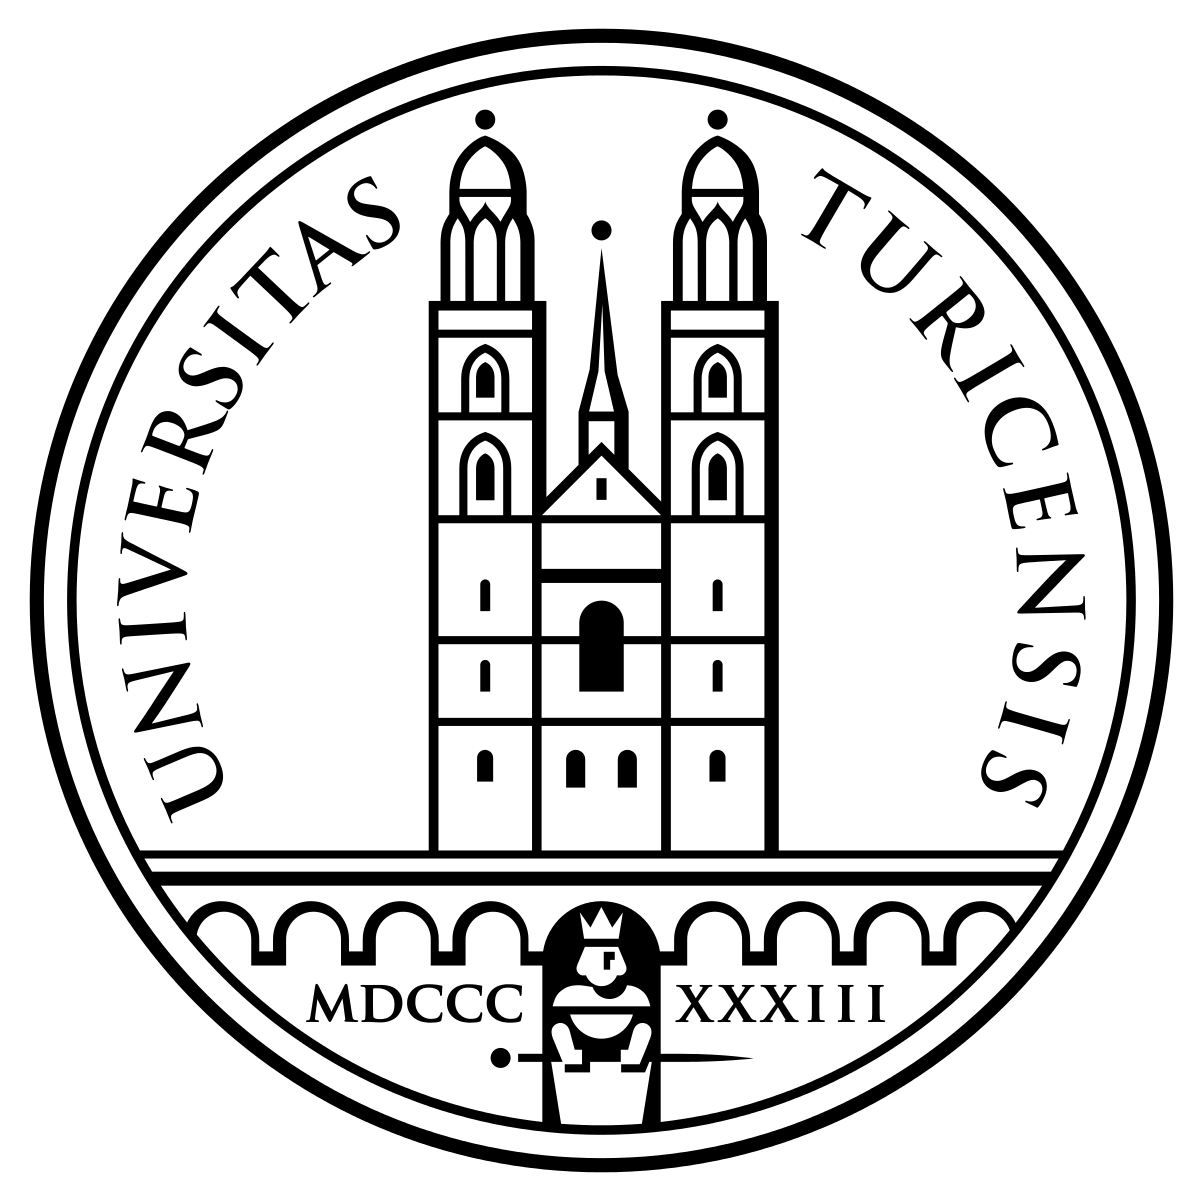
\includegraphics[width =0.34\textwidth]{UZH2.png}\\[1.2 cm]
      \textsc{\Large \textsc{Bachelorthesis}}\\[0.5 cm]

    \rule{\linewidth}{0.3 mm} \\[0.4cm]
    { \Large \bfseries Floquet dynamics of critical systems in one and higher dimensions}\\[0.3 cm]
    \rule{\linewidth}{0.3 mm} \\[1.5 cm]

  
    {\Large Fabian Jaeger}\\[2 cm] 
    
    
    		University of Zurich \\
             \textsc{Institute of Theoretical Physics} \\[1.5cm]
        
             	
    
    
    {\textbf{Supervised by}} \\[0.2cm]
   {\large  Prof. Dr. Titus Neupert} \\[2cm]
    
    {\large \today}\\[2 cm]
 
    \vfill
%    
%      \begin{minipage}{0.4\textwidth}
%        \begin{flushleft} \large
%            \textbf{Student}\\
%            \theauthor
%            \end{flushleft}
%            \end{minipage}~
%            \begin{minipage}{0.4\textwidth}
%            \begin{flushright} \large
%            \textbf{Enrollment Number} \\
%            17-740-325                                   % Your Student Number
%        \end{flushright}
%    \end{minipage}\\[1.2 cm]
    
\end{titlepage}

\begin{abstract}
    abstract-text
\end{abstract}

\newpage
\tableofcontents
\newpage


\section{Introduction}
% Write about the general field of Floquet Dyanmics

\section{Theory}
This section serves as an introduction into the tight-binding model, effects of boundary conditions on the measurement of relevant quantities, the sine-square deformation and the Floquet system we will be considering for this thesis. Even though for our considerations, the explicit details of the tight-binding model will not be relevant for most of the thesis, a brief overview is still provided.

\subsection{Tight-binding model}
In solid-state theory, there are many models used to describe the interactions of electrons and their respective atoms on a lattice. The model we will be considering in this thesis, is the so-called tight-binding model, in which the electrons are, in contrast to the free-electron model, modeled to be closely bound to their respective atoms. For a theoretical model, this has the useful consequence, that the interaction of other atoms in the crystal lattice with those tightly bound electrons, can be regarded as negligible.  This tight-binding of the electrons motivates, describing the electronic states as atomic orbital wave functions $\phi_A(\mathbf{r})$, rather than the commonly used plane waves $\exp(i \mathbf{k} \cdot \mathbf{r})$ from the free-electron model. Since the electrons are strongly localized to their respective atom, the atomic overlap of the atom wave functions of different atoms in the crystal lattice is therefore expected to be rather small. \\

%The description of the tight-binding is therefore equivalent to stating the the resulting atomic overlap of the wave functions on different atoms is small
%
%and that the resulting atomic overlap of the wave functions on different atoms is small.
It should be noted that the tight-binding approximation is mainly employed for describing low-lying electron energy states (i.e $s$- or $p$-orbitals) due to their lower spatial extension. In this regime, the  atomic potential plays a vital role and the electrons are not treated as free particles. The atomic Hamiltonian for an isolated Atom at position $\mathbf{R}$ is then given by:
\begin{equation}
	\hat{H}_A(\mathbf{r} - \mathbf{R}) = -\frac{\hbar^2}{2m}\nabla^2 + V_A(\mathbf{r} - \mathbf{R})
	\label{eq:single_atomic_potential}
\end{equation}
The functional dependence of the Hamiltonian on $\mathbf{r} - \mathbf{R}$ is due to the dependence of the rotationally symmetric Potential $V_A$ on the distance of the electron $\mathbf{r}$ of the position of the nucleus $\mathbf{R}$. Let $\ket{i, \mathbf{R}}$ be the relevant state for the atom at position $\mathbf{R}$ having the atomic wave function:
\begin{equation}
	\braket{\mathbf{r}}{i, \mathbf{R}_j} = \psi_A^i(\mathbf{r} - \mathbf{R})
\end{equation}
then the electrons will bind with eigenstates $\psi_A^i(\mathbf{r - \mathbf{R}})$ and $\epsilon_0 < 0$ which satisfy the equation:




% The atomic orbitals are solutions to the atomic Hamiltonian:
\begin{equation}
	\hat{H}_A \psi_A^i(\mathbf{r} - \mathbf{R}) = E_A^i \psi_A^i(\mathbf{r} - \mathbf{R})
\end{equation}
where $\psi_A^i(\mathbf{r} - \mathbf{R})$ represents the atomic orbital of energy level $i$ at Lattice position $\mathbf{R}$ and $E_A^i$ the resulting energy eigenvalue. \\

Our interest lies in modeling this for a lattice of atoms, meaning we want to consider the potentialfunction:
\begin{equation}
	V_\text{lattice}(\mathbf{r}) = \sum_{\mathbf{R}_i} V_A(\mathbf{r} - \mathbf{R}_i)
\end{equation}
 Extending our Hamiltonian to include the Coulomb interaction of the electron at position $\mathbf{r}$ with the nucleus of atoms at all possible position $\mathbf{R}_i$ of the crystal lattice, we get:
\begin{equation}
	\hat{H} = - \frac{\hbar^2}{2m} \nabla^2 + \sum_{\mathbf{R}_j} V_A(\mathbf{r} - \mathbf{R}_j) = \hat{H}_A + \Delta V_{\mathbf{R}_j}
\end{equation}
where in the second step we split the single atomic potential (\ref{eq:single_atomic_potential}), from the correction term:
\begin{equation}
	\Delta V_{\mathbf{R}_j}(\mathbf{r}) = \sum_{\mathbf{R}_i \neq \mathbf{R}_j} V_A(\mathbf{r} - \mathbf{R}_i)
\end{equation}

Electrons which are strongly bound to the atoms, i.e the ones with large binding energies, which correspond to low lying energy states in the spectrum shown in \ref{fig:illustration_tightbinding} will remain close to their host atoms. Those at higher energies, are more weakly bound and will be closer to free particles and able to tunnel to neighboring atoms due to an overlap of the corresponding wavefunction. The weakly bound electrons which become dislodged from their host atoms are called valence electrons (the same electrons which typically sit in the outer shells)

Since the electrons at the different positions of the atoms are mostly localized, they in essence are only strongly interacting with the nearest atomic potential at the position they are at. All other interactions resulting from the other atomic Potentials can be summarized in $\Delta V$, which can appropriately, in the tight-binding approximation, be seen as a small perturbation of the atomic potential at position $\mathbf{R}_j$ due to the coulomb repulsion of the other atoms at positions $\mathbf{R}_i$ on the crystal lattice. 
\begin{figure}[h]
	\centering
	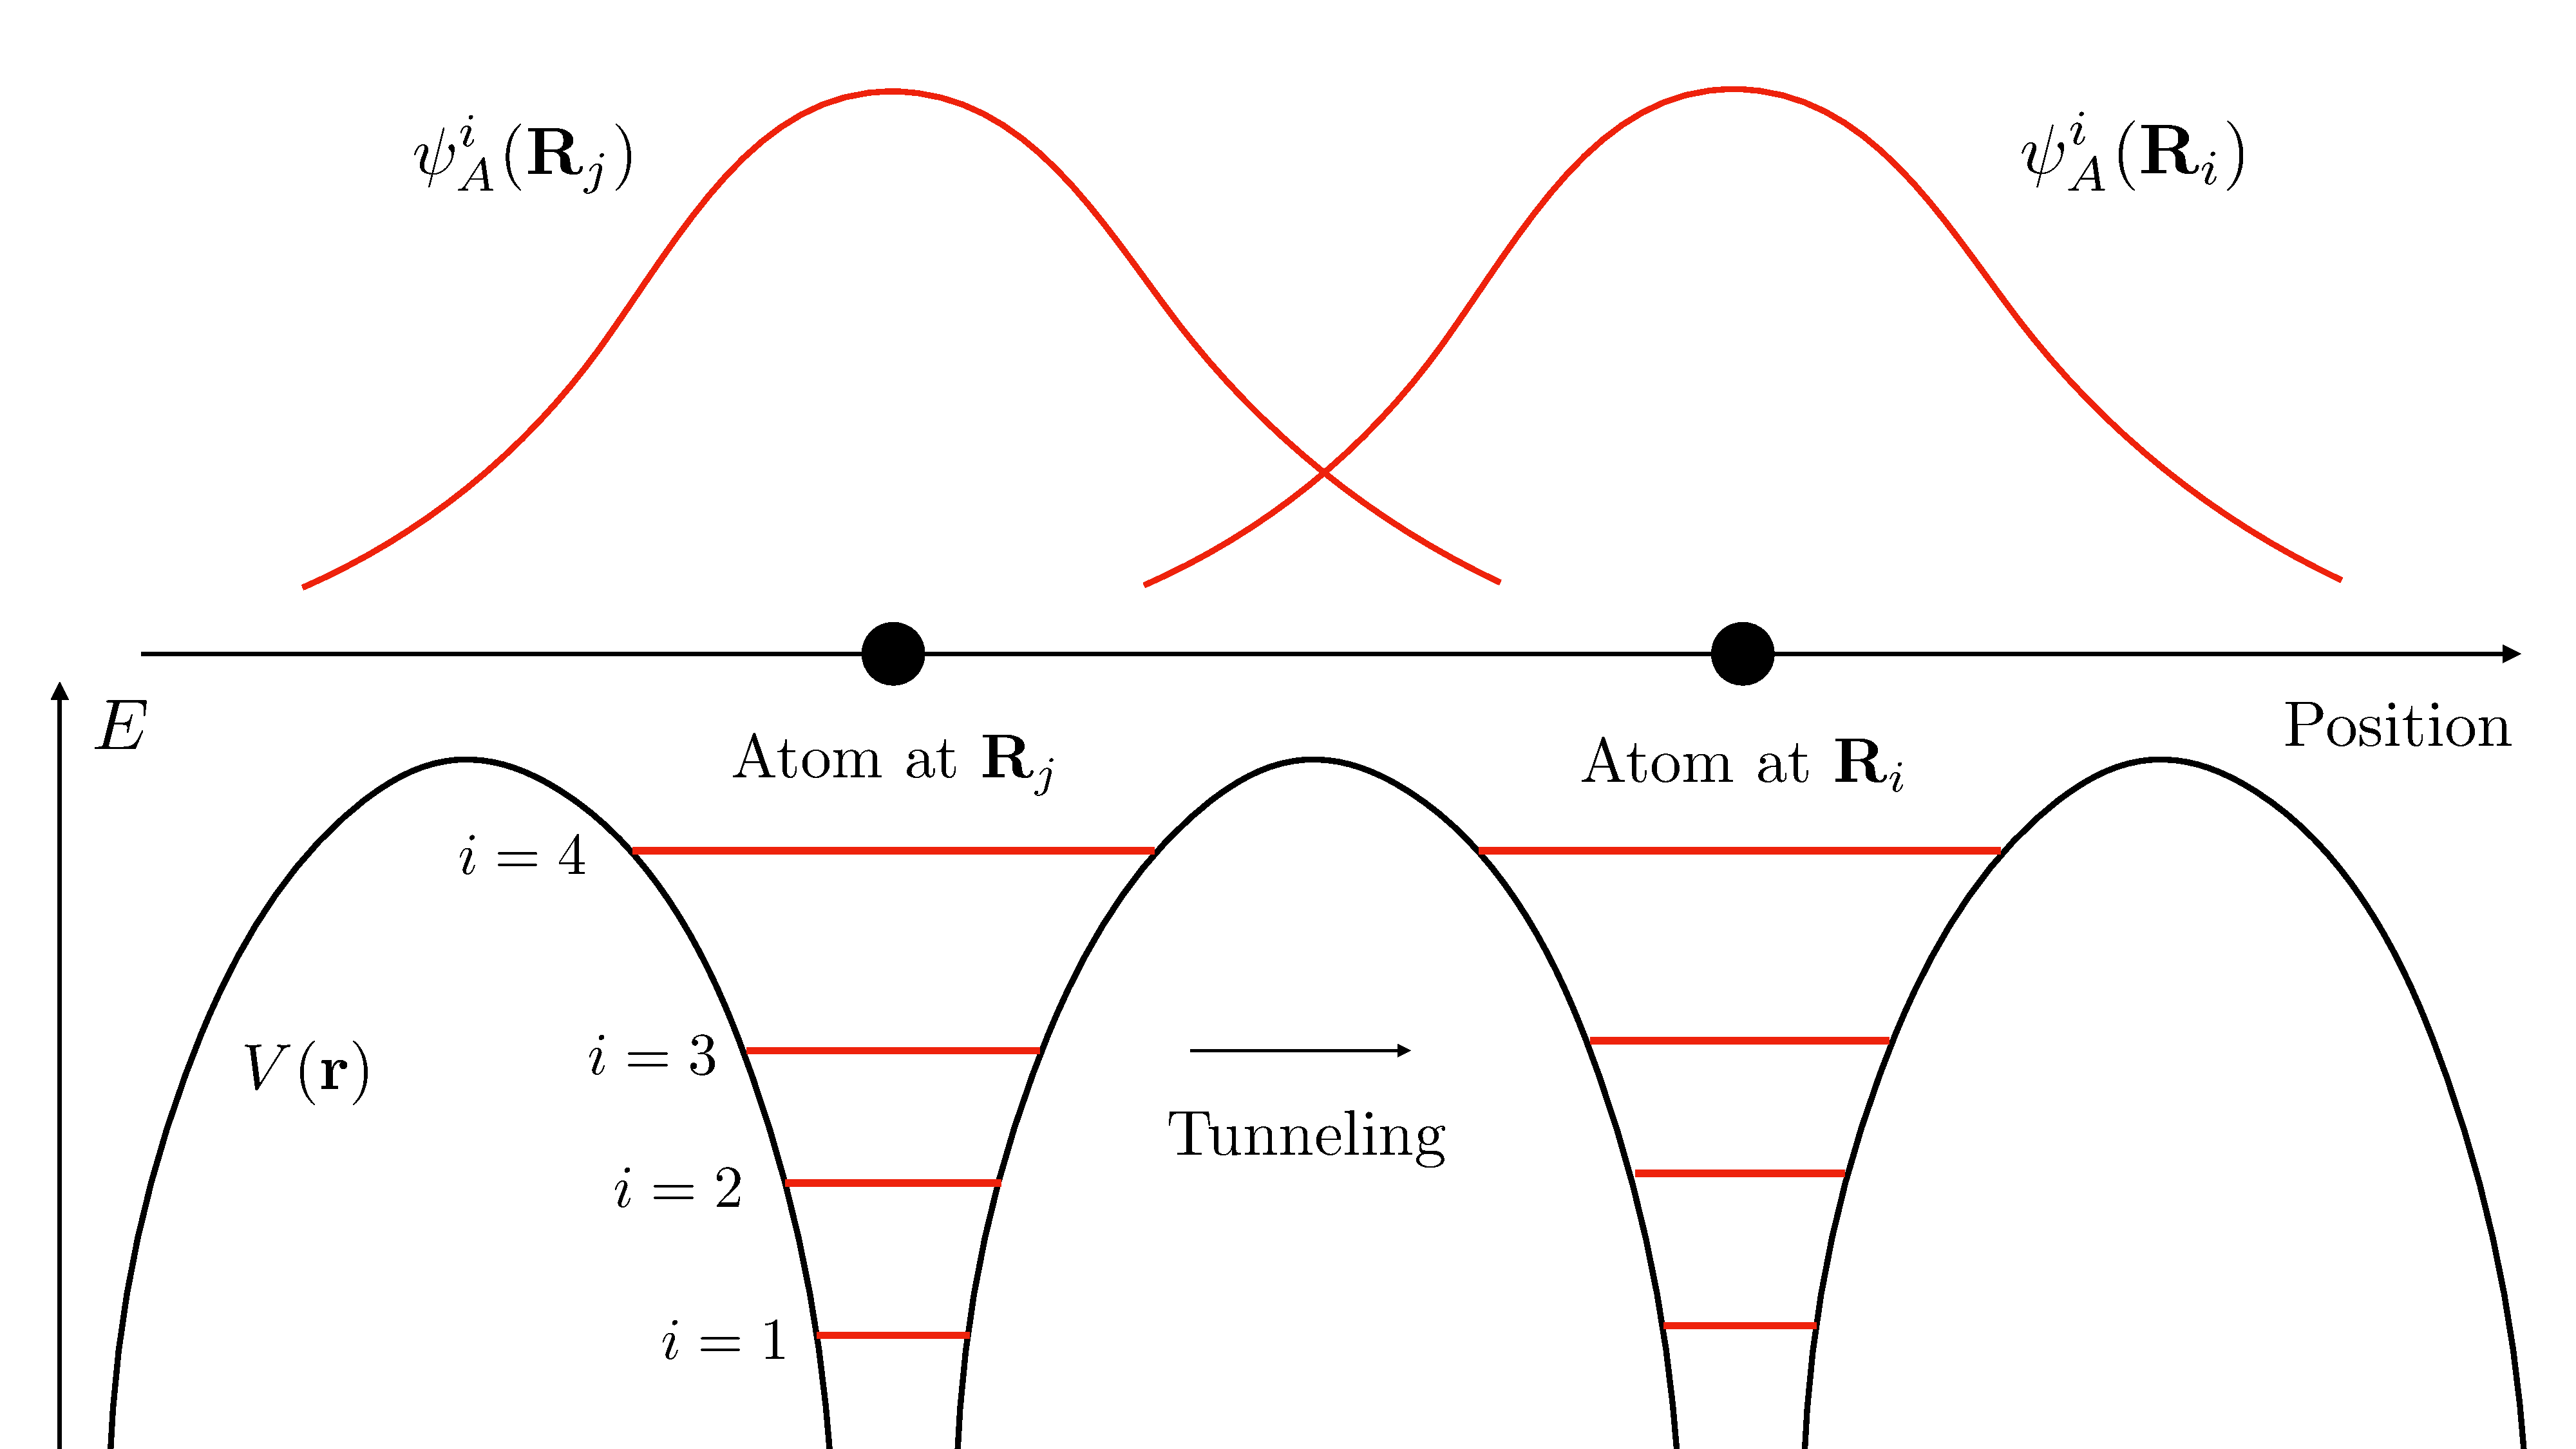
\includegraphics[width = 0.8\textwidth]{TightBindingModel-Illustration}
	\caption{Illustration of the tight-binding model}
	\label{fig:illustration_tightbinding}
\end{figure}
The advantage of such a procedure is that we have reduced our problem to a one-electron approximation, which can be solved with the help of a linear combination of atomic orbitals (LCAO):
\begin{equation}
	\psi_{n \mathbf{k}}(\mathbf{r}) = \frac{1}{\sqrt{N}} \sum_{\mathbf{R}_j} e^{i \mathbf{k} \cdot \mathbf{R}_j } \psi_{A}^i(\mathbf{r} - \mathbf{R}_j)
\end{equation} 
where the $\psi_A^i(\mathbf{r} - \mathbf{R}_j)$ are the atomic orbital wavefunctions obtained from (\ref{eq:single_atomic_potential}) when only one nucleus at present.  

% Needs to be rewritten, mostly copied from book Girvin
If we restrict our attention to this single orbital on each atom, then Bloch's theorem uniquely constrains the form of the eigenfunction in a Bravais lattice with lattice vector $\mathbf{k}$ to be
\begin{equation}
	\ket{\psi_{\mathbf{k}}} = \frac{1}{\sqrt{N}} \sum_{j=1}^N e^{i \mathbf{q} \cdot \mathbf{R}_j} \ket{\alpha, \mathbf{R}_j}
\end{equation}
To see why this is, consider
\begin{align}
	\braket{\mathbf{r}}{\psi_{\mathbf{k}}} &= \psi_{\mathbf{k}}(\mathbf{r}) = \frac{1}{\sqrt{N}} \sum_j e^{i \mathbf{k} \cdot \mathbf{R}_j} \phi_A^{\alpha}(\mathbf{r} - \mathbf{R}_j) \\
	&= e^{i \mathbf{k} \cdot \mathbf{r}} u_{\mathbf{k}}(\mathbf{r})
\end{align}
with
\begin{equation}
	u_{\mathbf{k}}(\mathbf{r}) = \frac{1}{\sqrt{N}} \sum_{j=1}^N e^{-i\mathbf{k} \cdot (\mathbf{r} - \mathbf{R}_j)} \phi_A^\alpha(\mathbf{r} - \mathbf{R}_j)
\end{equation}
We can check that the same periodicity of the potential $V(\mathbf{r} + \mathbf{a}) = V(\mathbf{r})$ holds for the function $u_{\mathbf{k}}(\mathbf{r} + \mathbf{a}) = u_{\mathbf{k}}(\mathbf{r})$
\begin{equation}
	u_k(\mathbf{r} + \mathbf{a}) = \frac{1}{\sqrt{N}} \sum_{j=1}^N e^{i \mathbf{k} \cdot (\mathbf{r} + \mathbf{a} - \mathbf{R}_j)} \phi(\mathbf{r} + \mathbf{a} - \mathbf{R}_j) = \frac{1}{\sqrt{N}} \sum_{i=1}^N e^{i \mathbf{k} \cdot (\mathbf{r} - \mathbf{R}_{i})} \phi_{A}^\alpha(\mathbf{r} - \mathbf{R}_i)
\end{equation}
which is equivalent to stating that $\psi_{\mathbf{k}}(\mathbf{k} + \mathbf{a}) =e^{i \mathbf{k} \cdot \mathbf{a}} \psi_{\mathbf{k}}(\mathbf{x})$.


Our main focus will be to obtain the explicit matrix form of this Hamiltonian. Let $\ket{\alpha, \mathbf{R}_j}$ be the ket for the atomic orbital, where $\alpha$ summarises all the relevant quantum numbers (such as the principal quantum number $n$, angular momentum $l$, and magnetic number $m$, for hydrogenlike atoms), then the matrix elements are given by:
\begin{equation}
	\mel{\alpha, \mathbf{R}_j}{\hat{H}}{\beta, \mathbf{R}_i} = E_{\alpha} \delta_{\alpha,\beta} \delta_{\mathbf{R}_j, \mathbf{R}_i} + \mel{\alpha,\mathbf{R}_j}{\Delta \hat{V}_{\mathbf{R}_j}}{\beta, \mathbf{R}_i}
\end{equation}
It should be noted that the solutions are not exakt but rather obtained using a variational approach. By increasing the amount of orbitals and therefore the Hilbert space we can improve the accuracy of the model. If we include more than one orbital per atom, i.e we do not simply have $\ket{\alpha,\mathbf{R}_j}$ but rather a set of $\alpha$'s per atomic site, the assumed orthogonality relation:
\begin{equation}
	\braket{\alpha, \mathbf{R}_j}{\beta, \mathbf{R}_j} = \delta_{\alpha\beta} \delta_{\mathbf{R}_j\mathbf{R}_i}
\end{equation}
The expected energy for the LCAO state is then the variational Ansatz \cite{Manfred}
%\begin{equation}
%	E(\mathbf{k}) = \frac{\mel{\psi_{n\
%\end{equation}
\subsection{Solution to tight-binding model in 1D}
To obtain our energy expectation values

\begin{equation}
	\mel{\alpha, \mathbf{R}_j}{\hat{H}}{\beta, \mathbf{R}_i} =  \epsilon_0 + \Lambda(\mathbf{k})
\end{equation}


which means for the matrix elements we consider
\begin{equation}
	H_{n,m} = \epsilon_0 \delta_{n,m} - t(\delta_{n+1, m} + \delta_{n-1},m)
\end{equation}

%\begin{equation}
%	\mel{\alpha, \mathbf{R}_j}{\Delta V_{\mathbf{R}_j}}{\beta, \mathbf{R}_i} = \begin{cases}
%		V_0 \quad 
%	\end{cases}
%\end{equation}


\subsection{Tight-binding model in second quantized formalism}
Restricting ourselves to the case where we consider only the lowest orbital and introducing the fermionic annihilation- $\hat{c}_{\mathbf{R}_j}$ and creation operators $\hat{c}^\dagger_{\mathbf{R}_j}$ at site with vector $\mathbf{R}_j$, the Hamiltonian is given by:
\begin{equation}
	\hat{H}_\text{tight-binding} = \sum_{j} E_0 \hat{c}_{\mathbf{R}_j}^\dagger \hat{c}_{\mathbf{R}_j} + \sum_{\mathbf{R}_i, \mathbf{R}_j} t_{ij} \hat{c}_{\mathbf{R}_i}^\dagger \hat{c}_{\mathbf{R}_j} + \text{h.c}
\end{equation}
The 'h.c' in this case denotes the hermitian conjugate, i.e the adjoint operator. The matrix elements $t_{ij} = t_{ji}$ are referred to as hopping elements where $t_{ij}^2$ determines the probability that an electron on site $i$ hops to site $j$. Since the operatorproduct $\hat{c}_i^\dagger \hat{c}_j$ annihilates an electron on site $\mathbf{R}_j$ and creates one on site $\mathbf{R}_i$, it represents the kinetic energy of the electron. Instead of considering all possible interactions with the potentials at all sites, we want to restrict ourselves to identical nearest neighbor interactions at every position $\mathbf{R}_j$, meaning we set:
\begin{equation}
	t_{ij} = \mel{\mathbf{R}_j}{\Delta \hat{V}_{\text{atom}, \mathbf{R}_j}}{\mathbf{R}_l} = \begin{dcases}
		-t \quad &\text{if $\mathbf{R}_j$ and $\mathbf{R}_l$ are nearest neighbors }\\
		0 \quad & \text{otherwise}
		\end{dcases}
\end{equation}
and we obtain the following final form for our tight-binding Hamiltonian:
\begin{equation}
	\hat{H}_{\text{tight-binding}} = - t \sum_{\expval{\mathbf{R}_j, \mathbf{R}_i}} \hat{c}_{\mathbf{R}_j}^\dagger \hat{c}_{\mathbf{R}_l} + \text{h.c} = -\frac{t}{2} \sum_{i}\sum_{\mathbf{\delta}} (\hat{c}_i^\dagger \hat{c}_{i + \mathbf{\delta}} + \hat{c}_{i + \mathbf{\delta}}^\dagger \hat{c}_i)
	\label{eq:general_tight_binding}
\end{equation}
where in the second step we expanded the nearest neighbor sum $\expval{ij}$ and inserted the 1/2 to avoid double counting. The sum $\sum_{\mathbf{\delta}}$ sums over all the nearest neighbor vectors of $\mathbf{\delta}_1, \mathbf{\delta}_2, \dots \mathbf{\delta}_q$. In my work (as we will not consider diagonal hopping for $d \geq 2$) we simply have $q = 2d$ where $d$ is the dimension of the Bravais lattice. \\

%\begin{equation}
%	t_{ij} = \mel{\mathbf{R}_j}{\Delta \hat{V}_{\text{atom, \mathbf{R}_j}}}{\mathbf{R}_l} = \begin{dcases}
%		-t \quad &if $\mathbf{R}_j$ and $\mathbf{R}_l$ are nearest neighbors \\
%		0 \quad &otherwise
%	\end{dcases}
%\end{equation}

It should be noted that in general one would have to include the spin degrees of freedom but we will consider a simplified model without spins in this thesis, meaning only strictly one electron can exist at any given lattice site.

\subsubsection{Diagonalization of Hamiltonian with Periodic Boundary Conditions}

We consider a change of basis to the momentum space representation. A change of Basis for a second-quantized operator is given by
\begin{equation}
	\hat{c}_\alpha^\dagger = \sum_\beta \braket{\beta}{\alpha} \hat{c}_\beta^\dagger \qq{and} \hat{c}_\alpha = \sum_\beta \braket{\alpha}{\beta} \hat{c}_\beta
\end{equation}
where $\{\ket{\alpha} \}$ and $\{\ket{\beta}\}$ are a full set of orthonormal basis states that span the hilbert space. A projection
onto the Fourier space (which is equivalent to the transformation between Bloch and Wannier functions, we get the following
\begin{equation}
	\braket{\mathbf{k}}{j} = \psi_{\mathbf{k}}^*(\mathbf{r}_j) = \frac{1}{\sqrt{N}} e^{-i \mathbf{k} \cdot \mathbf{r}_j} \qq{and} \braket{j}{\mathbf{k}} = \psi_\mathbf{k}(\mathbf{r}_j) = \frac{1}{\sqrt{N}} e^{i \mathbf{k} \cdot \mathbf{r}_j}
\end{equation}
resulting in the following creation and annihilation operators in momentum space:
\begin{equation}
	\hat{c}_{\mathbf{k}} = \frac{1}{\sqrt{N}}  \sum_{\mathbf{k}} e^{-i \mathbf{k}\cdot \mathbf{r}_j} \hat{c}_{\mathbf{k}}^\dagger \qq{and} \hat{c}_\mathbf{k} = \frac{1}{\sqrt{N}} \sum_\mathbf{k} e^{i \mathbf{k} \cdot \mathbf{r}_j} \hat{c}_\mathbf{k}
\end{equation}
where the sum over momentums $\mathbf{k}$ is taken over the first brillouin zone. In 1D, this would mean, $\mathbf{k} = 2\pi n/ N$ with $n = 0, \dots, N$ where $L = Na$.
which inverted yields us:
\begin{equation}
	\hat{c}_j = \frac{1}{\sqrt{N}} \sum_{\mathbf{k}} e^{i \mathbf{k}\cdot \mathbf{r}_j} \hat{c}_\mathbf{k} \qq{and} \hat{c}_j^\dagger = \frac{1}{\sqrt{N}} \sum_{\mathbf{k}} e^{-i\mathbf{k}\cdot \mathbf{r}_j} \hat{c}_\mathbf{k}^\dagger
\end{equation}
The diagonalized Hamiltonian in momentum space can then be writen as
\begin{equation}
	\hat{H}_{\text{tight-binding}} = \sum_{\mathbf{k}} \epsilon_{\mathbf{k}} \hat{c}_{\mathbf{k}}^\dagger \hat{c}_{\mathbf{k}}
\end{equation}
with the energy disperion of a free particle:
\begin{equation}
	\epsilon_{\mathbf{k}} = \frac{p^2}{2m} = \frac{\hbar^2 \abs{\mathbf{k}}^2}{2m}
\end{equation}

Strictly speaking in a general tight-binding model we will additionally have to take into account the chemical potential $\mu$. For the one-dimensional lattice we therefore obtain
\begin{equation}
	\hat{H} = - t \sum_{j=1}^{L-1} \hat{c}_j^\dagger \hat{c}_{j+1} + \hat{c}_{j + 1}^\dagger \hat{c}_j - \mu \hat{c}_j^\dagger \hat{c}_j - \alpha t( \hat{c}_{L}^\dagger \hat{c}_1 + \hat{c}_1^\dagger \hat{c}_L)
\end{equation}
The parameter $\alpha$ serves to specify which boundary conditions we are using. For OBC we have $\alpha = 0$ and for PBC, $\alpha = 1$.  \\

 

Using the above transformation, the Hamiltonian \ref{eq:general_tight_binding} becomes
\begin{equation}
	\hat{H}_{tb} = - \frac{t}{2N} \sum_j \sum_{\mathbf{\delta}, \mathbf{k}, \mathbf{k}'} (e^{-i \mathbf{k} \cdot \mathbf{R}_i} e^{i \mathbf{k}' \cdot (\mathbf{R}_i + \mathbf{\delta})} \hat{c}^\dagger_{\mathbf{k}} \hat{c}_{\mathbf{k}'} + e^{-i \mathbf{k}' \cdot (\mathbf{R}_j + \mathbf{\delta})} e^{i \mathbf{k} \cdot \mathbf{R}_j} \hat{c}_{\mathbf{k}}^\dagger \hat{c}_{\mathbf{k}'} )
\end{equation}
Now using the relation
\begin{equation}
	\sum_{\mathbf{k}} e^{i(\mathbf{k} - \mathbf{k}')\mathbf{R}_j} = N \delta_{\mathbf{k},\mathbf{k}'}
\end{equation}
we obtain
\begin{equation}
	\hat{H}_{tb} = -\frac{t}{2} \sum_{\mathbf{\delta}, \mathbf{k}} (e^{i\mathbf{k} \cdot \mathbf{\delta}} + e^{-i\mathbf{k} \cdot \mathbf{\delta}})\hat{c}_{\mathbf{k}}^\dagger \hat{c}_{\mathbf{k}} = -t \sum_{\mathbf{k}, \mathbf{\delta}} \cos(\mathbf{k}\cdot \mathbf{\delta}) \hat{c}_{\mathbf{k}}^\dagger \hat{c}_{\mathbf{k}}
\end{equation}
The momentum-space representation of the tight-binding Hamiltonian is therefore
\begin{equation}
	\hat{H}_{tb} = \sum_{\mathbf{k}} \epsilon_{\mathbf{k}} \hat{c}_{\mathbf{k}}^\dagger \hat{c}_{\mathbf{k}}
\end{equation}
where
\begin{equation}
	\epsilon_{\mathbf{k}} = -t \sum_{\mathbf{\delta}} \cos(\mathbf{k} \cdot \mathbf{\delta})
\end{equation}
is the system's energy dispersion relation.


\begin{equation}
	\epsilon(l) = \begin{cases}
		- 2t\cos(\frac{\pi l}{N+1}) &\qq{for OBC } (\alpha = 0) \\[10pt]
		- 2t\cos(\frac{2\pi l}{N}) &\qq{for PBC } (\alpha = 1)
	\end{cases}
\end{equation}
Often more compactly we write $\epsilon(k) = -2t\cos(ka)$ where the states with $k < 0$ represent electrons moving to the right and $k>0$ electrons moving to the left.



\subsection{Solution to tight-binding model}


The solution of a tight binding models of atoms, each having a single atomic orbital, on a square lattice is given by
\begin{equation}
	E(k) = \epsilon_0 - 2t\cos(k_x a) - 2t\cos(k_ya)
\end{equation}
In principle, the calculations can be made more precise by including more atomic orbitals in our LCAO approximations per unit cell.


\begin{figure}[h]
\centering
\begin{subfigure}[t]{0.49\textwidth}
	\centering
	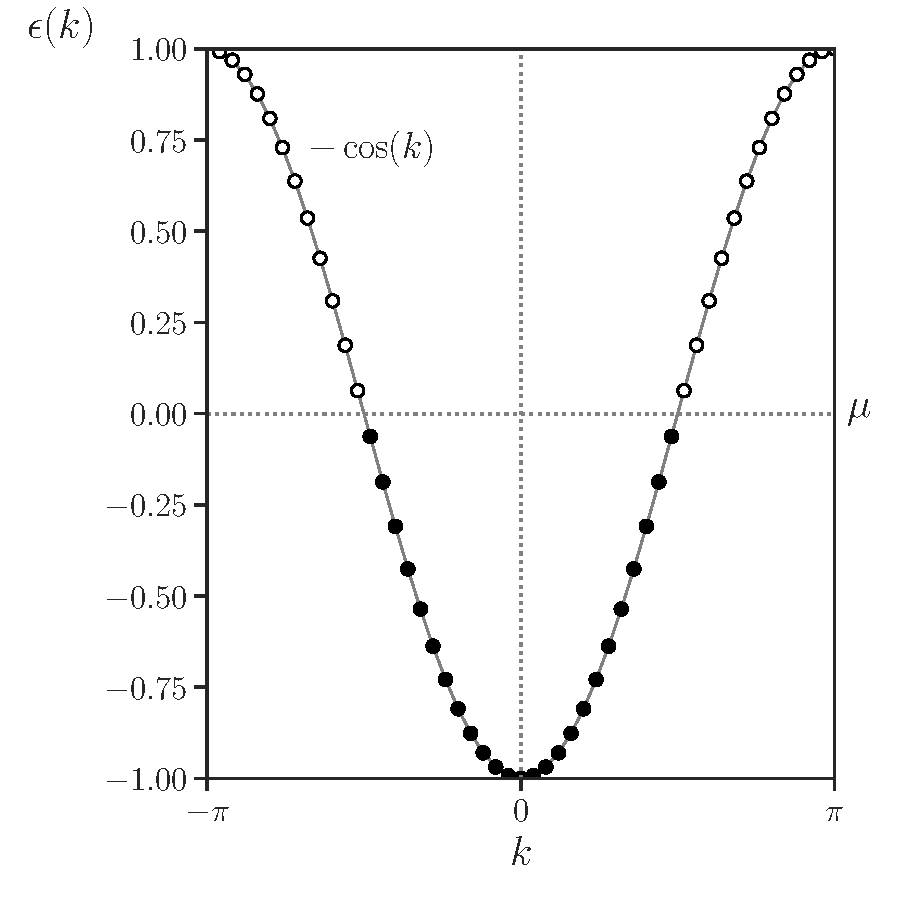
\includegraphics[width =\textwidth]{dispersionrelationH0}\end{subfigure}
\begin{subfigure}[t]{0.49\textwidth}
	\centering
	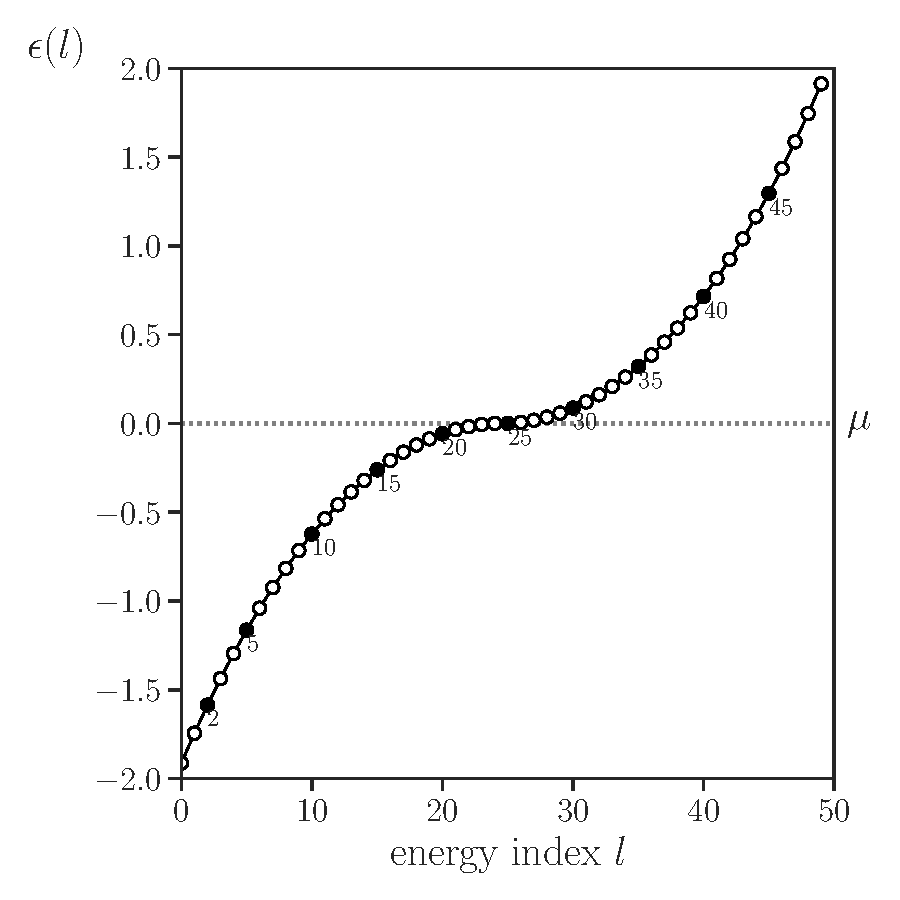
\includegraphics[width =\textwidth]{dispersionrelationSSD}
\end{subfigure}
\caption{(left) Dispersion relation $\epsilon(k) = -2t\cos(ka)$ for the tight-binding Hamiltonian for $L=50$, chemical potential $\mu = 0$, lattice constant $a = 1$ and hopping parameter $t = 1/2$. Represented is half-filled ground state occupation up to the Fermi level $\epsilon_F = \mu =0$ for spin-less fermions. (right) energy-eigenvalues for the sine-squared deformed Hamiltonian $\hat{H}_{\text{SSD}}$ for $L = 50$ and $\mu = 0$.}
\end{figure}




\section{Boundary Conditions and Sine-Square Deformation}
In finite systems such as the models treated in this thesis the choice of boundary conditions will have a direct effect on the properties of the system. In general, there are two choices of boundary conditions, periodic-boundary conditions and open-boundary conditions. In general, open boundary conditions introduce boundary oscillations such as Friedel oscillations, One way to suppress such effects is through the introduction of so-called smooth boundary conditions. In an SSD system, the Hamiltonian is deformed according to the rescaling function
\begin{equation}
	f_x = \sin^2\left[\frac{\pi}{L} \left(x -\frac{1}{2} \right)\right]
	\label{eq:scaling_function_SSD}
\end{equation}
% We used a slightly modified function
where $x$ is the local position and $L$ is the length of the system. It can be shown that applying the sine-square deformation to the one-dimensional free fermion system with open boundary conditions completely removed unwanted boundary effects such as the Friedel oscillation. This resulted in completely position-independent two-point correlation functions such as the bond-strength and particle density in the ground state. 



Boundary Conditions have a great effect on the observed quantities for a chain. In the case for example with open-boundary conditions (OBC) results in boundary-induced modulation such as Friedel Oscillation. \\

In this thesis we will consider Open-boundary conditions (OBS) and periodic boundary conditions (PBC). To suppress boundary energy corrections the introduction of so called smooth boundary conditions such as the sine-squared deformation greatly reduce these effects for a one-dimensional free fermion chain. For periodic boundary conditions, the system is translationally invariant. Surprisingly, even though the sine-squared deformation breaks the translational invariance, it can be shown that they share the same \\

As can be seen in the spatial dependence of the correlation function $\expval{\hat{c}_j^\dagger \hat{c}_{j+1} + \hat{c}_{j+1}^\dagger \hat{c}_j}$ at half filling with $N=100$ in Figure (\ref{BondEnergy}), the sine-squared deformed Hamiltonian greatly reduces the Friedel Oscillations imposed by open boundary conditions. \\


%TODO Rewrite this better
It can be readily be verified that the condition for the total number of particles in the system $N_g$:
\begin{equation}
	N_g = \sum_{i=0}^{L-1} \expval{n_i}
\end{equation}
holds. In a translationally invariant system such as the one with periodic boundary conditions, the occupation numbers $\expval{n_i}$ are spatially uniform quantities, corresponding to $N_g/L$ respectively.


\subsection{Sine-square deformation in momentum space}
The construction of the sine-squared deformed Hamiltonian for a one-dimensional $L$ lattice chain with periodic boundary condition, is done through the introduction of a chiral deformation 
\begin{equation}
	\hat{H}^{(\pm)} = - t \sum_{j=1}^L e^{\pm i \delta x} [\hat{c}_j^\dagger \hat{c}_{j+1} + \text{h.c}] - \mu \sum_{j=1}^L e^{\pm i \delta(x - 1/2)} \hat{c}^\dagger_j \hat{c}_j
\end{equation}
where for completeness the chemical potential is also included and $\delta = 2\pi/L$. As is evident, the chiral Hamiltonian represent simply the Fourier transformation of each term in the sum. The sine-squared deformed tight-binding Hamiltonian can then be constructed as follows:
\begin{equation}
	\hat{H}_{\text{SSD}} = \frac{1}{2} \hat{H}_0 - \frac{1}{4} \left[\hat{H}^{(+)} + \hat{H}^{(-)}\right] = -t \sum_{j=1}^{L} f\left(j + \frac{1}{2}\right)[\hat{c}^\dagger_j \hat{c}_{j+1} + \text{h.c}] - \mu \sum_{j=1}^L f(j) \hat{c}_j^\dagger \hat{c}_j
	\label{eq:SSD_Hamiltonian_chiral}
\end{equation}
where $f(i)$ corresponds to the scaling function defined in \ref{eq:scaling_function_SSD}. \\


In the $k$-Basis where the original tight-binding Hamiltonian is diagonal, with our definition of our creation and destruction operators, the chiral Hamiltonian takes the form:
\begin{equation}
	\hat{\mathcal{H}}^{(\pm)} = \sum_k e^{\mp i \delta/2} \epsilon(k \mp \delta/2) \hat{c}_k^\dagger \hat{c}_{k \mp \delta}
\end{equation}
This Hamiltonian induces momentum transfers $\Delta \delta k = \pm \delta$ only for nearest neighbor sites in $k$ space. Notably, applying the chiral Hamiltonian on the Fermi sea of the tight-binding model, only processes across the Fermi point $k = \pm k_F$ are allowed since most of the momentum transfers are forbidden due to the Pauli exclusion principle.

\begin{figure}[h]
	\centering
	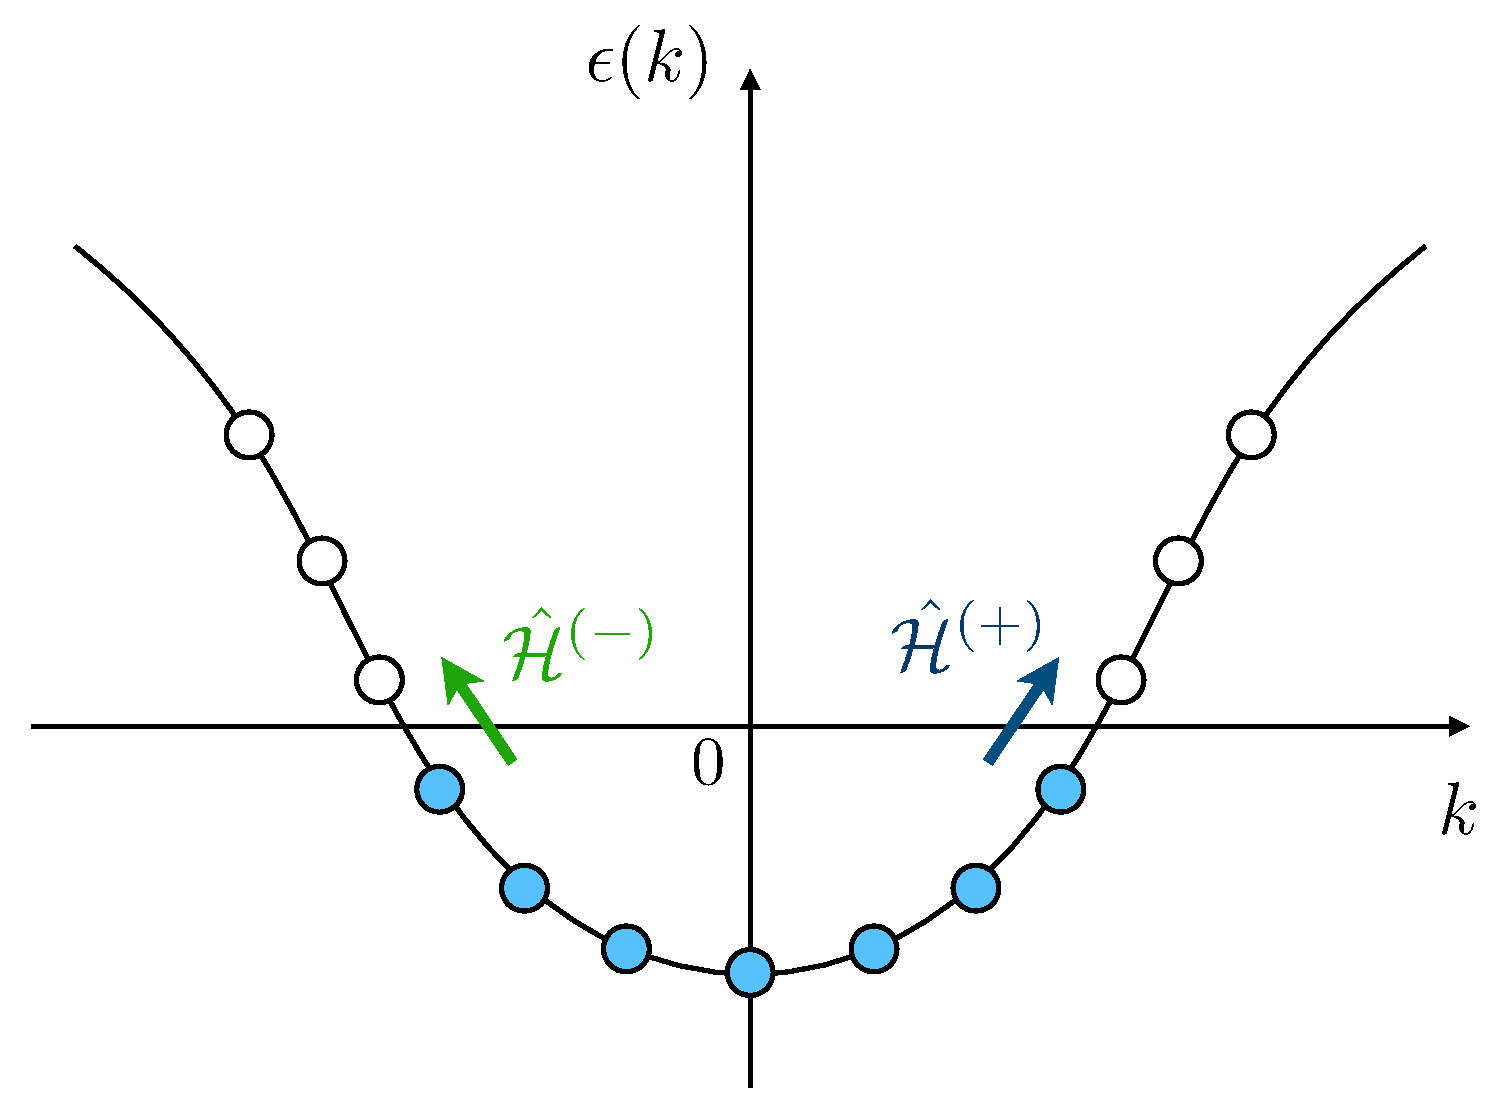
\includegraphics[width=0.6\textwidth]{SSD_Construction}
	\caption{Schematic representation of the allowed chiral $\hat{\mathcal{H}}^{(+)}$ (blue arrow) and anti-chiral $\hat{\mathcal{H}}^{(-)}$ (green arrow) excitations in momentum space. Due to the Pauli Principle these processes are heavily restricted and only processes at the Fermi momentum $k_F$ are allowed.}
\end{figure}

It turns out that by fine-tuning the chemical potential $\mu$ such that $\epsilon(k_F \mp \delta/2) = 0$, the active processes across the fermi point can be neglected, which means that the fermi sea of the tight-binding model with periodic boundary conditions is also an exact eigenstate of the chiral Hamiltonian and therefore of the sine-squared deformed Hamiltonian \ref{eq:SSD_Hamiltonian_chiral}. In addition to being an eigenstate, it can be shown, that the Fermi sea corresponds to the exact ground state of the SSD Hamiltonian \cite{Katsura} \cite{Maruyama}.

\subsubsection{In two-dimensions}
The construction of the sine-squared deformed Hamiltonian in two-dimensions follows analogously to the one-dimensional case via the introduction of the chiral Hamiltonian. In our numerical calculations we will mainly restrict ourselves to a 2d square lattice with non-diagonal hopping. Letting $t_1$ correspond to the hopping in $x$-direction and $t_2$ in $y$ direction, the chiral Hamiltonian takes the form:
\begin{equation}
\begin{split}
	\hat{H}^{(\pm)} = &-t_1 \sum_{\mathbf{r}} \exp(\pm i[\delta_x x + \delta_y( y - 1/2)]) \left[\hat{c}^\dagger(x,y) \hat{c}(x+1, y) + \text{h.c}\right] \\
		&- t_2 \exp(\pm i [\delta_x(x-1/2) + \delta_y y]) \left[\hat{c}^\dagger(x,y) \hat{c}(x, y+1) + \text{h.c} \right]
\end{split}
\end{equation}
the tight-binding model with periodic boundary conditions imposed in both directions will take the form:
\begin{equation}
\begin{split}
\hat{H}_0 =  \sum_{i = 1}^{L_x} \sum_{j=1}^{L_y}& -\frac{t_1}{2} \left[ \hat{c}^\dagger(i, j) \hat{c}(i+1, j) + \hat{c}^\dagger(i+1, j)\hat{c}(i, j) \right] \\
	&-\frac{t_2}{2} \left[\hat{c}^\dagger(i,j) \hat{c}(i,j+1) + \hat{c}^\dagger(i, j+1)\hat{c}(i,j) \right] \\
	& - \mu \left[ \hat{c}^\dagger(i,j) \hat{c}(i,j)\right]
\end{split}
\end{equation}
In a similar fashion, the chiral Hamiltonian can be diagonalized in momentum space:
\begin{equation}
	\hat{\mathcal{H}}_{\mathbf{\delta}}^{(\pm)} = \sum_{\mathbf{k}} e^{\mp i/2(\delta_x + \delta_y)} \epsilon(\mathbf{k} + \mathbf{\delta}/2)\hat{c}_{\mathbf{k}}^\dagger \hat{c}_{\mathbf{k} \mp \mathbf{\delta}}
\end{equation}
which again allows describes the processes connecting the sites $\mathbf{k}$ and $\mathbf{k} \pm \mathbf{\delta}$. The difference to the 1d case however here is that $\epsilon(\mathbf{k} + \mathbf{\delta}/2) = 0$ cannot be achieved by tuning the parameter $\mu$ which means that the Fermi sea is only an approximate eigenstate of the chiral Hamiltonian and the correspondence exists only in the thermodynamic limit $L_{x,y} \rightarrow \infty$.


This expresssion is best generalized as a sum over two indices. We best define the square lattice with the help of the coordinate tuple $(i, j)$ meaning our Hamiltonian takes the form
\begin{equation}
	\hat{H}_0 =  \sum_{i = 1}^{L_x} \sum_{j=1}^{L_y} -\frac{t_1}{2} \left[ \hat{c}^\dagger(i, j) \hat{c}(i+1, j) + \hat{c}^\dagger(i+1, j)\hat{c}(i, j) \right] - \frac{t_2}{2} \left[\hat{c}^\dagger(i,j) \hat{c}(i,j+1) + \hat{c}^\dagger(i, j+1)\hat{c}(i,j) \right]
\end{equation}



For our SSD Deformed Hamiltonian we use the following product:
\begin{equation}
	\mathcal{F}(x,y) = f_x(x)f_y(y) = 4\sin(\frac{\pi x}{L})^2\sin(\frac{\pi y}{L})^2
\end{equation}
and the Sine-squared Hamiltonian takes the form
\begin{equation}
\begin{split}
\hat{H}_\text{SSD} = \sum_{i=1}^{L_x} \sum_{j=1}^{L_y} &t_1 \mathcal{F}\left(x+\frac{1}{2}, y\right) \left[ \hat{c}^\dagger(x,y)\hat{c}(x+1, y) + \hat{c}^\dagger(x+1,y) \hat{c}(x,y)\right] \\
&+ t_2 \mathcal{F}\left(x, y+ \frac{1}{2}\right) \left[\hat{c}^\dagger(x, y) \hat{c}(x, y + 1) + \hat{c}^\dagger(x, y+1) \hat{c}(x,y) \right]
\end{split}
\end{equation}
Which we will formulate with the help over a sum over two indices $i$ and $j$:
\begin{equation}
	\begin{split}
		\hat{H}_\text{SSD} = \sum_{i=1}^{L_x} \sum_{j=1}^{L_y} &t_1 \mathcal{F}\left(i+\frac{1}{2}, j\right) \left[ \hat{c}^\dagger(i,j)\hat{c}(i+1, j) + \hat{c}^\dagger(i+1,j) \hat{c}(i,j)\right] \\
&+ t_2 \mathcal{F}\left(i, j + \frac{1}{2}\right) \left[\hat{c}^\dagger(i, j) \hat{c}(i, j + 1) + \hat{c}^\dagger(i, j+1) \hat{c}(i,j) \right]
	\end{split}
\end{equation}
%\begin{figure}[h]
%	\centering
%	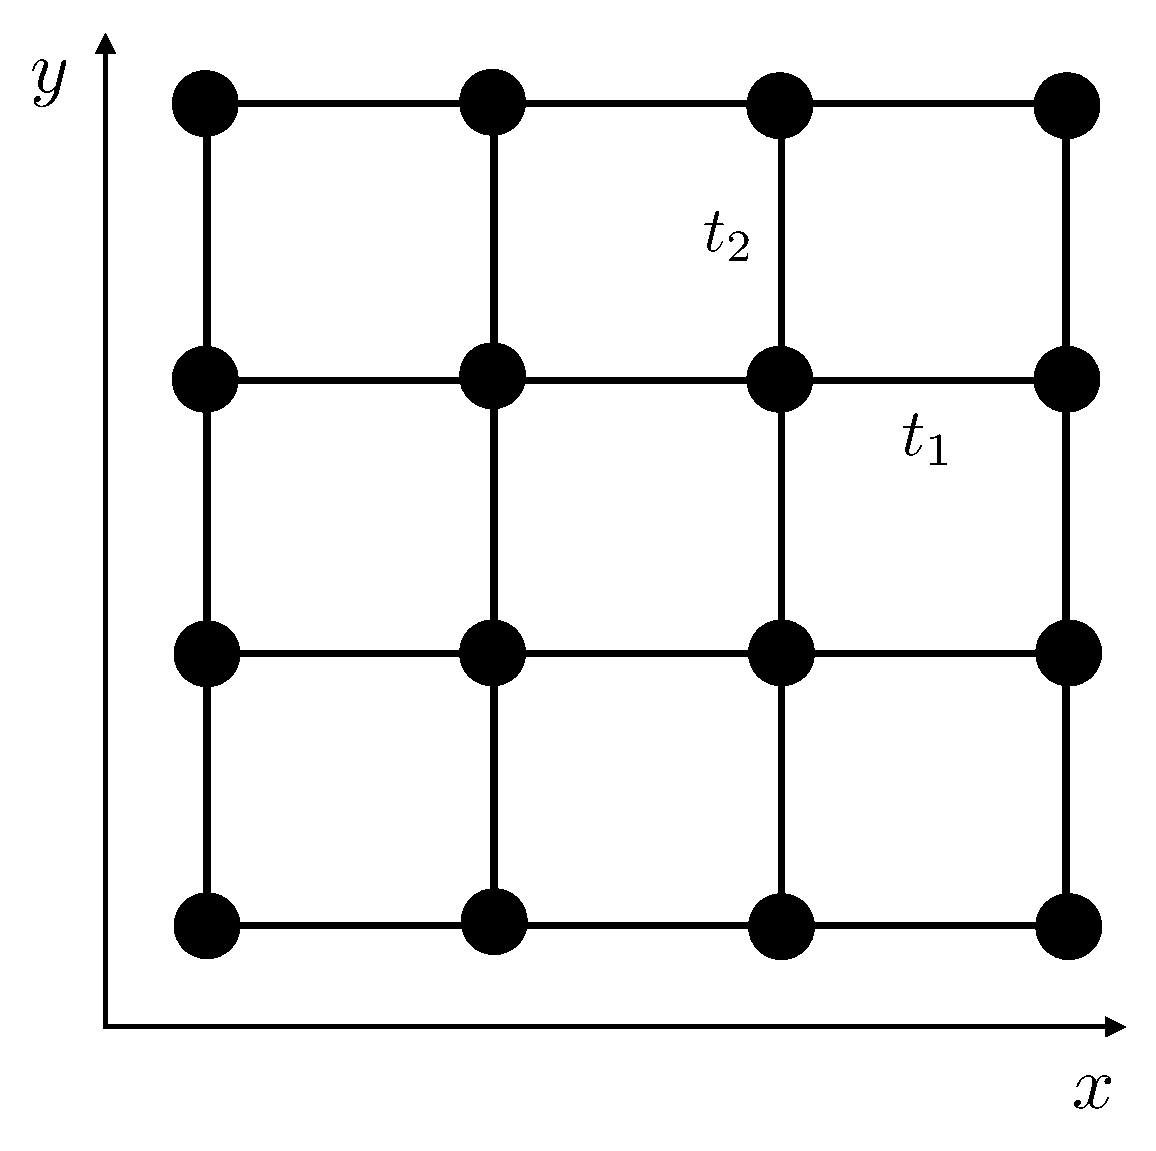
\includegraphics[width = 0.4\textwidth]{Square_Lattice}
%	\caption{}
%\end{figure}

%\begin{figure}
%	\centering
%	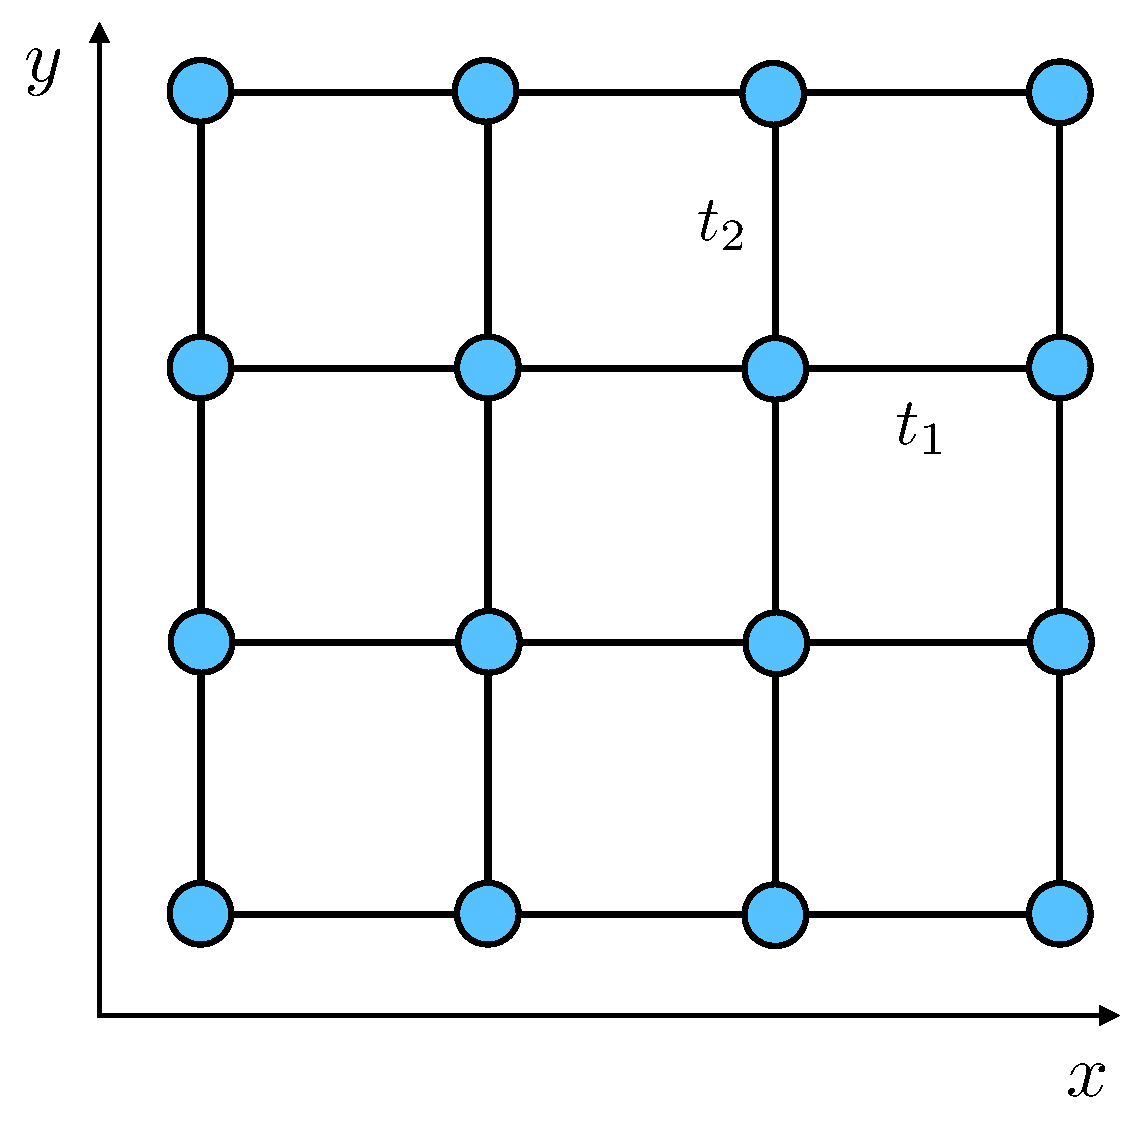
\includegraphics[width = 0.8\textwidth]{Square_Lattice2}
%	\caption{}
%\end{figure}


\subsubsection{Energy corrections}

For open boundary conditions the ground state energy at half filling is obtained by summing up all the negative eigenvalues:
\begin{equation}
	E_O^{N} = \sum_{i = 1}^{N/2} \epsilon_m = t\left[1 - \left(\sin(\frac{\pi/2}{N+1}) \right)^{-1} \right]
\end{equation}
The subscript in this case will denote the different possible cases, $O$ for OBC, $P$ for PBC and $S$ for SSD.
Expanding the right hand side with respect to $N$, one finds the form
\begin{equation}
	\frac{E_O^N}{N} \sim - \frac{2 t}{\pi} + \frac{t}{N}\left( \frac{2}{\pi} - 1\right) + \mathcal{O}\left(\frac{1}{N^2}\right)
\end{equation}
Compared with the energy per site in the thermodynamic limit:
\begin{equation}
	\lim_{N \rightarrow \infty} \frac{E_O^N}{N} = \frac{1}{\pi} \int_{0}^{\pi/2} -2t \cos(k) \dd k = - \frac{2}{\pi} t 
\end{equation}
where we chose the integration limit to be from 0 to $\pi/2$ to include all $k$-modes with negative Energies in the case for $N \rightarrow \infty$. That this holds can be seen from the dispersion relation. The finite-size correction to the energy per site (or even the energy per bond) is of the order of $1/N$.


It is expected that the ratio $E_S^N/ B^N$ rapidly converges to $-2t/\pi$ which is the expectation value $\expval{c_j^\dagger c_{j+1}^\dagger + \hat{c}_{j+1}^\dagger \hat{c}_j}$ in the thermodynamic limit, which in the case of $t = -1/2$ corresponds to the $0.636$ seen in the plot (\ref{BondEnergy}) 
%\begin{equation}
%	
%\end{equation}


%\begin{equation}
%	\mel{0}{\hat{c}_m}{i} = \frac{1}{\sqrt{N}} \exp[i
%\end{equation}

\subsubsection{Periodic Boundary Conditions}
For periodic boundary conditions the Hamiltonian is given by
\begin{equation}
	\hat{H}_P = -t\sum_{i=1}^{N-1} \left( \hat{c}_i^\dagger\hat{c}_{i+1} + \hat{c}^\dagger_{i+1} \hat{c}_i\right) - t\left(\hat{c}_N^\dagger \hat{c}_1 + \hat{c}_i^\dagger \hat{c}_N\right)
\end{equation}

\begin{equation}
	\ket{\Psi} = \frac{1}{\sqrt{N}} \sum_{\mathbf{R}} e^{i\mathbf{k} \cdot \mathbf{R}} \phi_n(\mathbf{r} - \mathbf{R}_j)
\end{equation}
where $\phi_n$ represents the atomic orbitals. \\


As we know from Bloch's theorem, eigenstates of a periodic Hamiltonian can be presented in the form of Bloch waves $\psi_{\mathbf{k}}(\mathbf{r}) = e^{i\mathbf{k}\cdot \mathbf{r}} u_{\mathbf{k}}(\mathbf{r})$ where the components of the crystal momentum $\mathbf{k}$ take values inside the Brillouin zone, $k_i \in [-\pi/a, \pi/a]$ where we assumed that periodicity of the lattice potential is the same in all directions, i.e $V(\mathbf{r} + a\mathbf{e}_i) = V(\mathbf{r})$.

It can readily be verified that this Linear combination of atomic orbitals satisfies the Bloch theorem, which is to be expected since the underlying lattice potential is periodic. \\


The tight-binding approximation (for a single band) greatly simplifies the problem by reducing the Hilbert space to one atomic orbital per atom. As a result, instead of working with the full Bloch wave function that depends on the continuous variable $\mathbf{r}$, we need only work with the amplitude of the state on atom $j$, which we call $\psi_j$. The full Bloch wave function is constructed from $\psi_j$ and the orthonormal local orbital $\ket{j}$ (we neglect the orbital or band index to simplify notation in this subsection). In many cases the coarse-grained physical properties of the electron states depend mostly on $\psi_j$ but not sensitively on the details of the orbital wave function $\phi(\mathbf{r})$, so often $\phi_j$ is the focus of the study and viewed as the wave function itself.


So instead of considering the case
\begin{equation}
	\ket{\Psi_{\mathbf{k}}} = \sum_j \psi_j \ket{j}
\end{equation}
For a Bravais lattice, the discrete translation symmetry dictates that
\begin{equation}
	\psi_j = \frac{1}{\sqrt{N}} e^{i \mathbf{k} \mathbf{R}_j}
\end{equation}

As an Ansatz we use the plane wave solution:
\begin{equation}
	\psi_m = \frac{e^{-ikNa}}{\sqrt{N}}
\end{equation}
where $N$ denotes the lattice site and $a$ represents the lattice constant, meaning Length is $L = Na$, the allowed values of $k$ are quantized in units of $2\pi/L$. Due to periodic boundary conditions, we impose a condition over the allowed values of $k$
\begin{equation}
	e^{ikNa} = 1 \Rightarrow k = \frac{2\pi}{Na}m, \quad m:\text{ integer}
\end{equation}
In this case, the one-particle wave function is the plane wave
%\begin{equation}
%	\psi_
%\end{equation}


\subsubsection{In one-dimension}
For a one-dimensional lattice of length $L$ and lattice constant $a = 1$, the general tight-binding Hamiltonian (\ref{eq:general_tight_binding}) takes the form:
\begin{equation}
	\hat{H}_{\text{tight-binding}} =  - \frac{t}{2} \sum_{i=1}^{L-1} \hat{c}_i^\dagger \hat{c}_{i+1} + \hat{c}_{i+1}^\dagger \hat{c}_i
\end{equation}
where we set the nearest neighbor vectors to be $\delta_1 = a$ and $\delta_2 = -a$.

	\begin{figure}[h]	
		\centering
		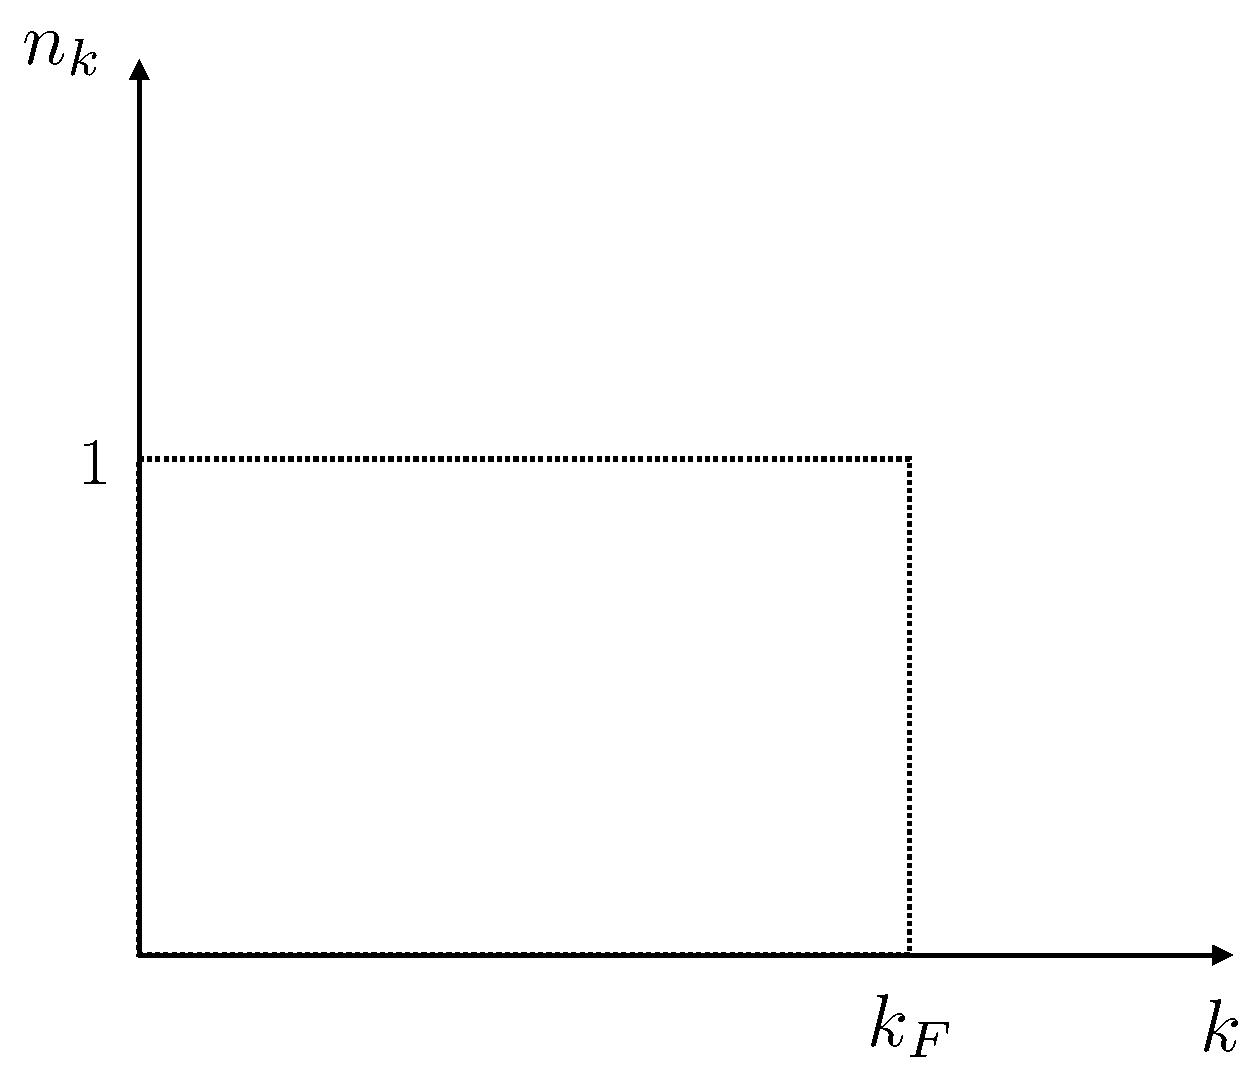
\includegraphics[width=0.8\textwidth]{Disperion_relation1D}
		\caption{Dispersion relation and Occupation for a free fermion system (without spins) in one-dimension}
	\end{figure}
	
	
\begin{figure}[h]
\centering
\begin{subfigure}[t]{0.49\textwidth}
	\centering
	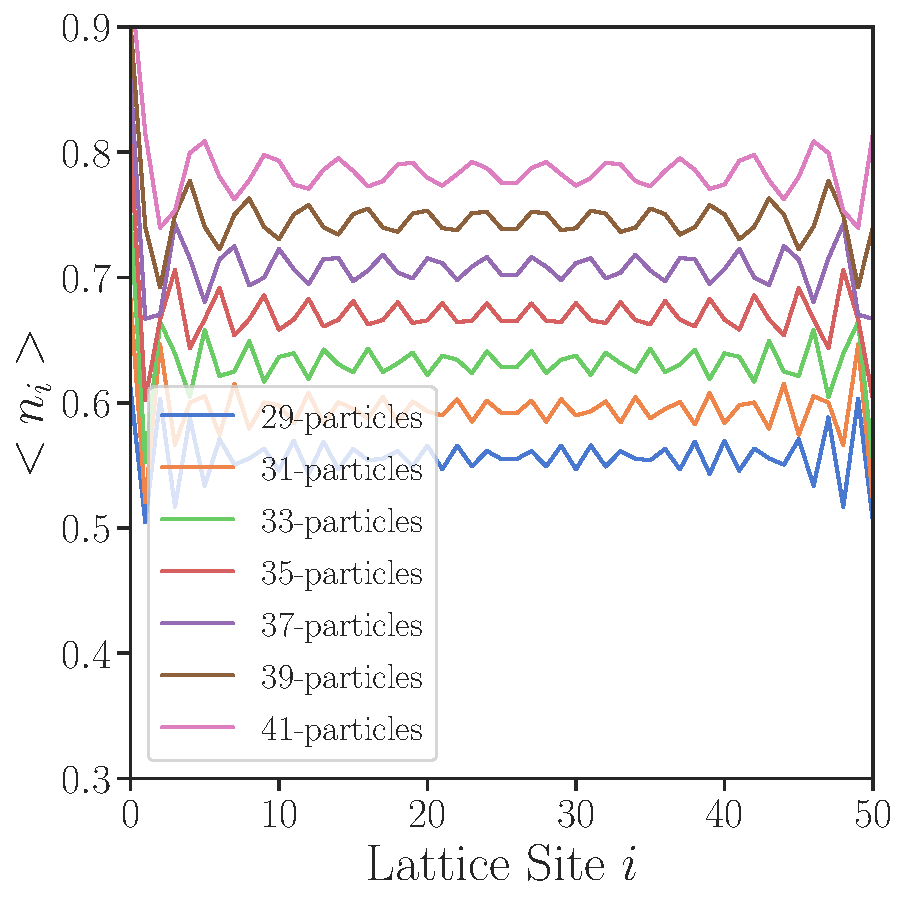
\includegraphics[width =\textwidth]{Occupation_number_H0_OBC}
	\caption{}
\end{subfigure}
\begin{subfigure}[t]{0.49\textwidth}
	\centering
	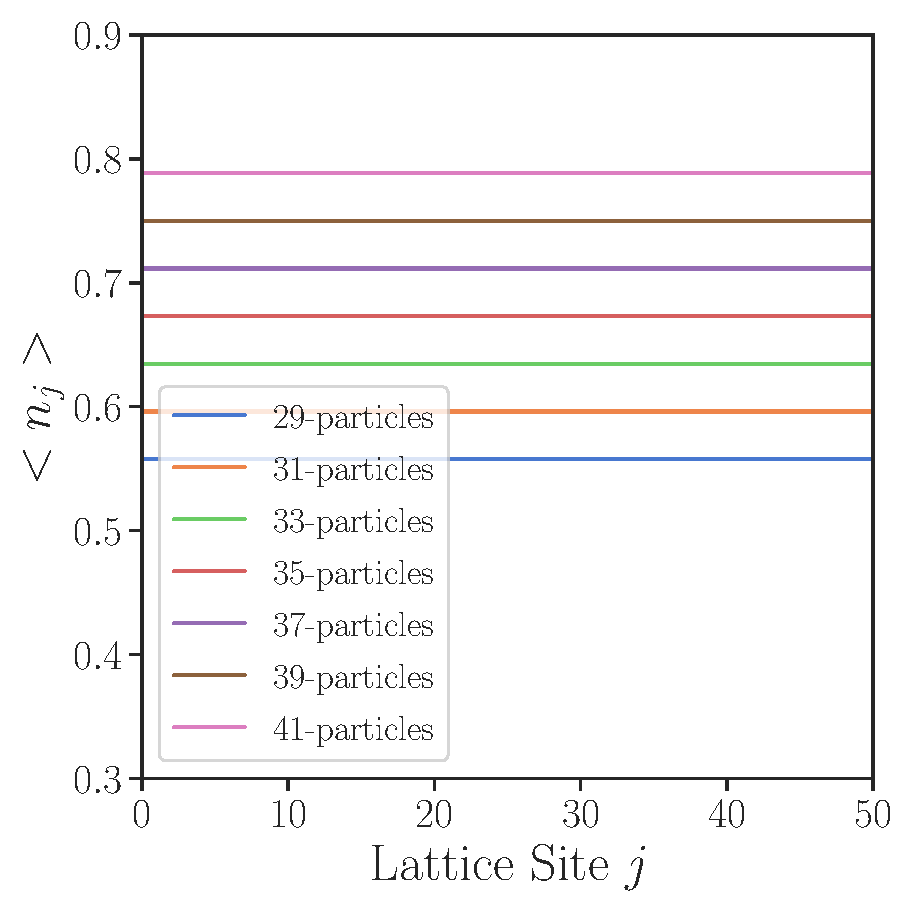
\includegraphics[width =\textwidth]{Occupation_number_H0_PBC}
	\caption{}
\end{subfigure}
\caption{}
\end{figure}



\begin{figure}[h]
\centering
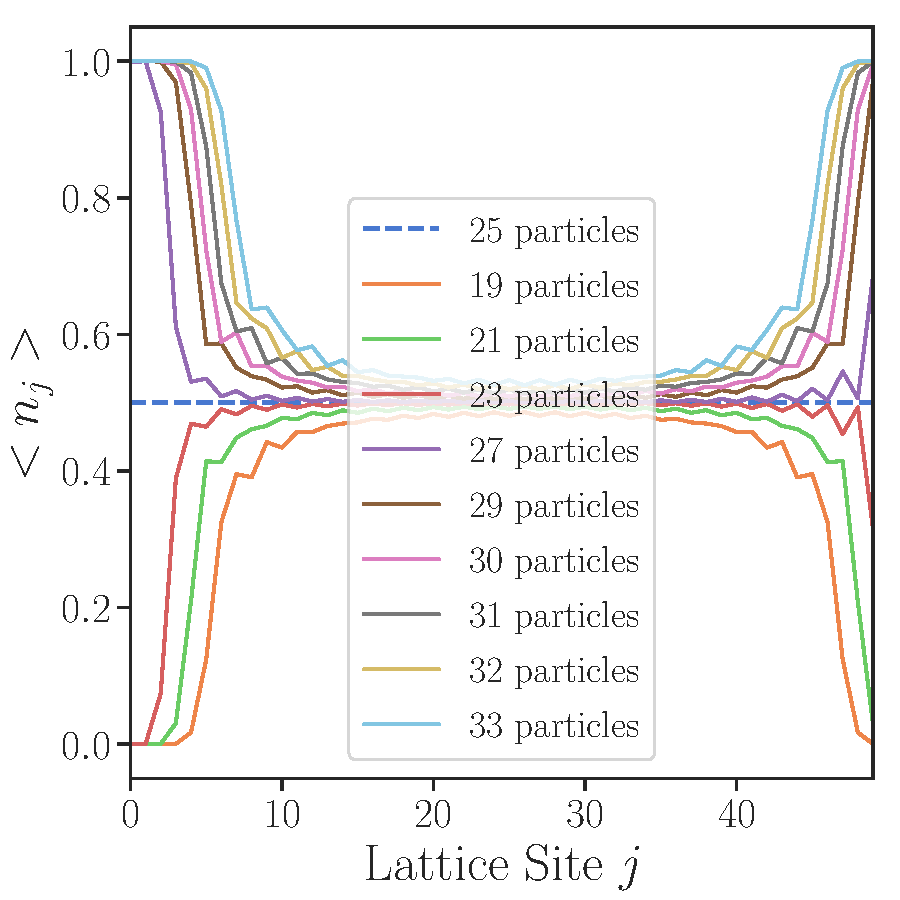
\includegraphics[width=0.9\textwidth]{Occupation_number_H1}
\caption{The Occupation number $n_i(\epsilon_l) = \abs{\varphi_{l,i}}^2$ as a function of the energy index $l$ and the lattice site close to the chemical potential $\mu = 0$ for $L = 50$.}
\end{figure}




\begin{figure}[h]
	\centering
	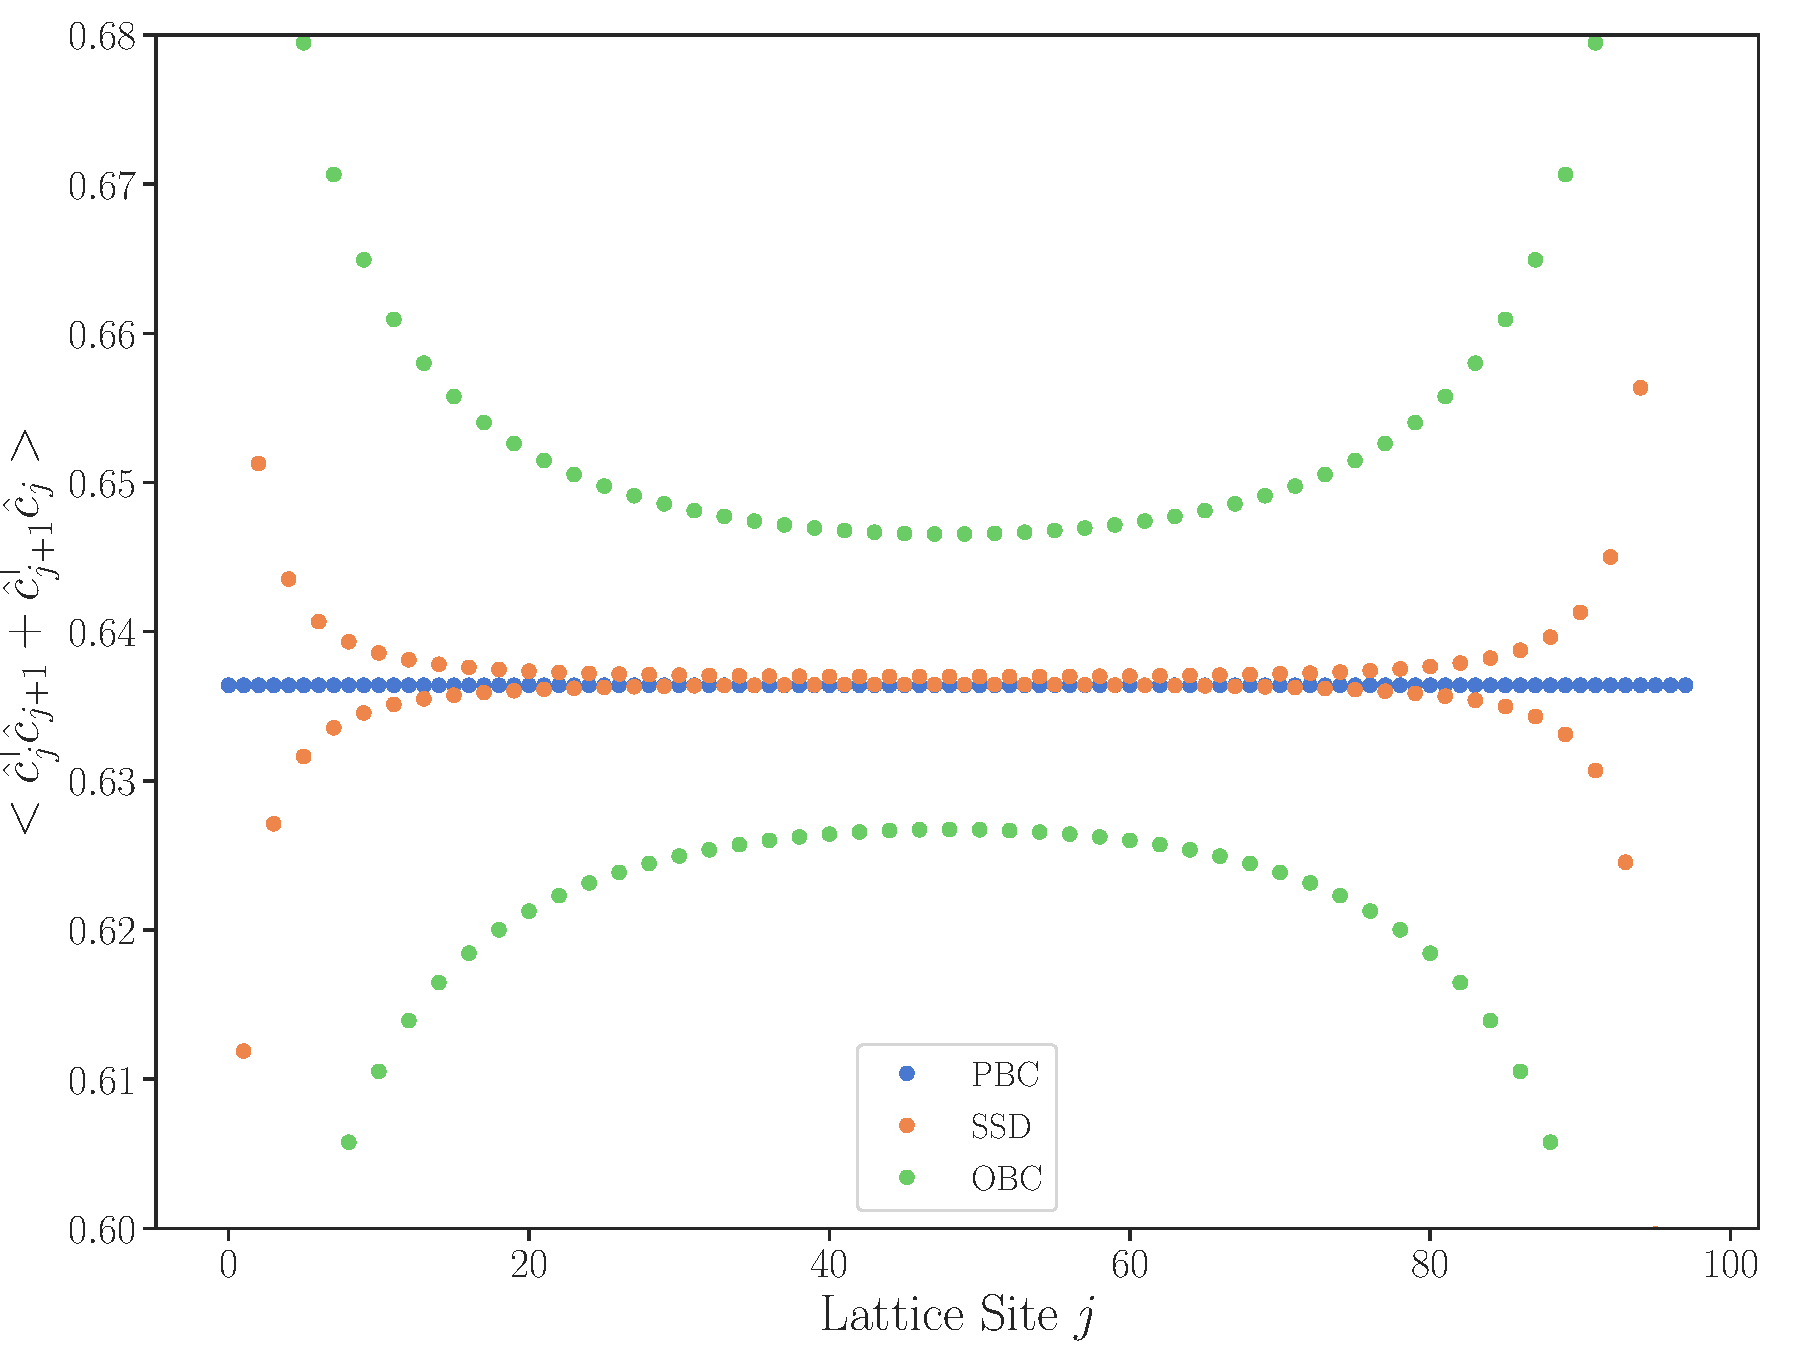
\includegraphics[width=0.8\textwidth]{BondEnergy}
	\caption{Expectation Value of the Bond Energy in the Ground state with half filling as a function of the lattice site}
	\label{BondEnergy}
\end{figure}

\subsubsection{in Two-dimensions}

	\begin{figure}[h]
		\centering
		\begin{subfigure}[t]{0.49\textwidth}
		\centering
			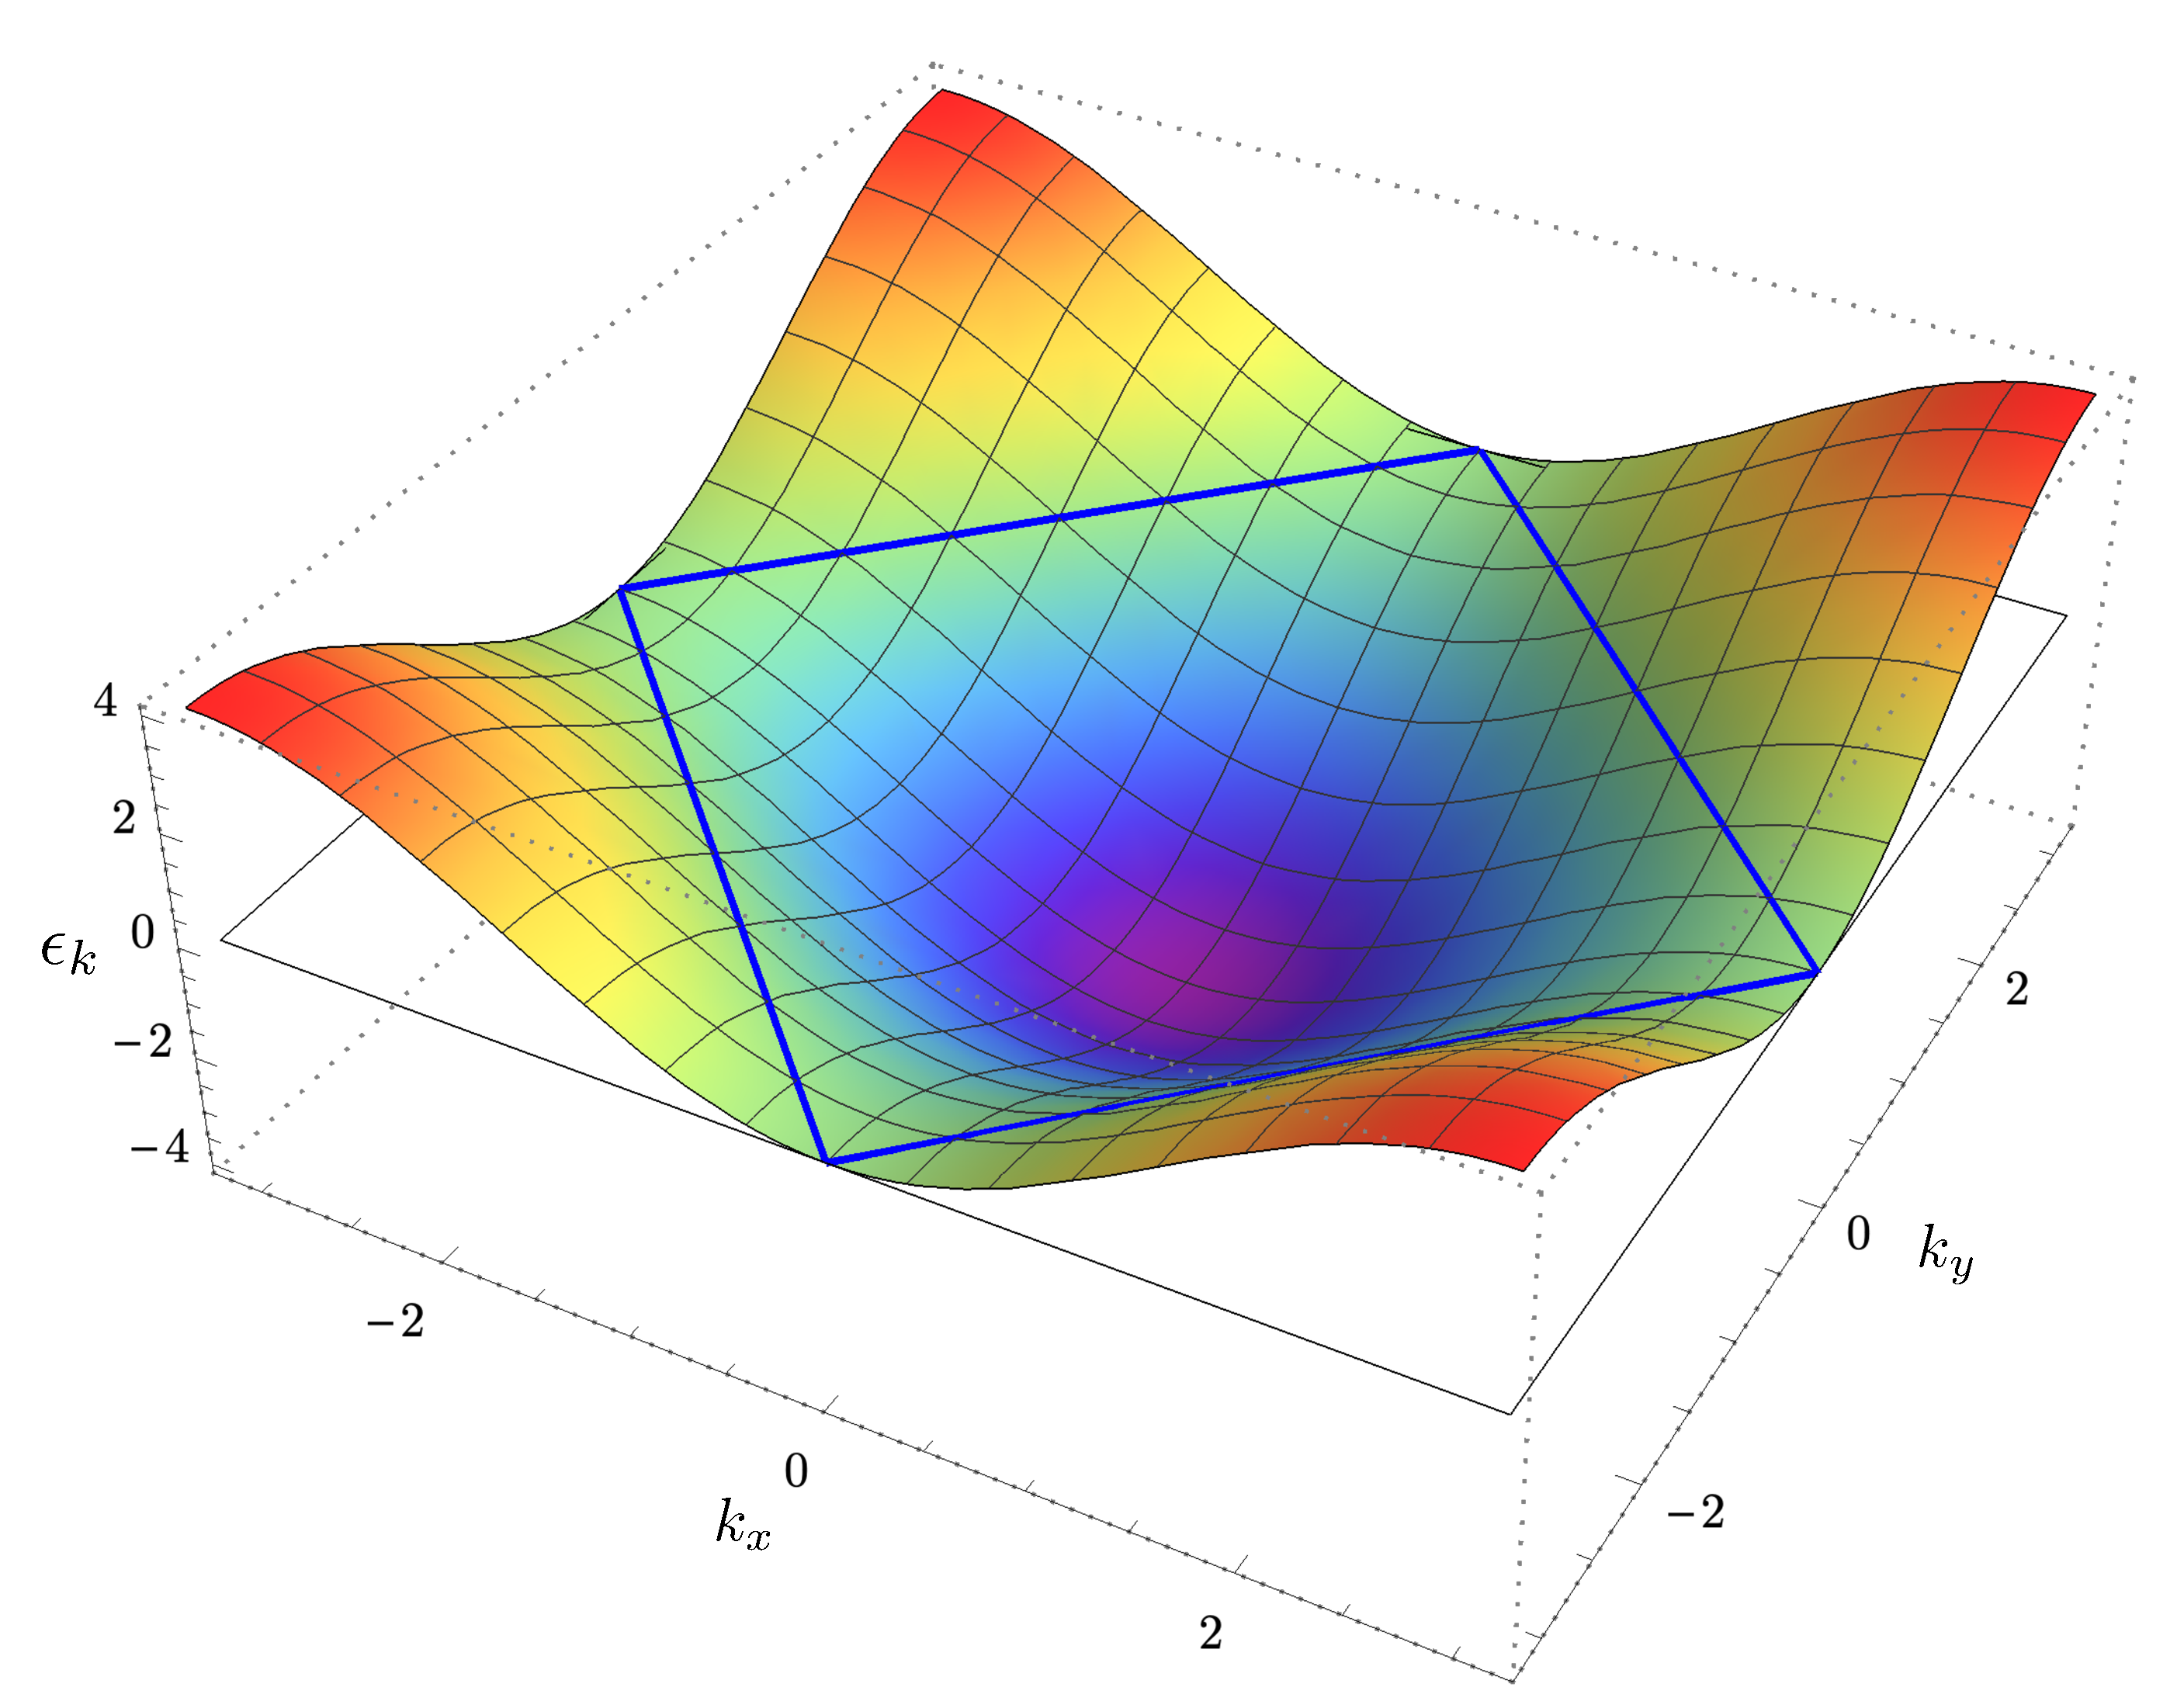
\includegraphics[width =\textwidth]{Dispersion_relation2d}
			\caption{}
		\end{subfigure}
		\begin{subfigure}[t]{0.49\textwidth}
		\centering
			\includegraphics[width =0.8\textwidth]{Dispersion_Relation2d_Top}
			\caption{}
		\end{subfigure}
		\caption{Dispersion Relation for a 2D tight binding Hamiltonian; (a) Dispersion relation for the tight binding Hamiltonian in two-dimensions. Up to the blue lines around the Energy $\epsilon_k = 0$ the states are filled in the ground state. The Fermi surface separates the occupied states from the non-occupied ones. Here displayed is the first brillouin zone}
	\end{figure}

\subsection{Sine-Squared deformation Hamiltonian}


\subsection{Floquet Systems}


\begin{figure}[h]
\centering
		\begin{subfigure}[b]{0.45\textwidth}
			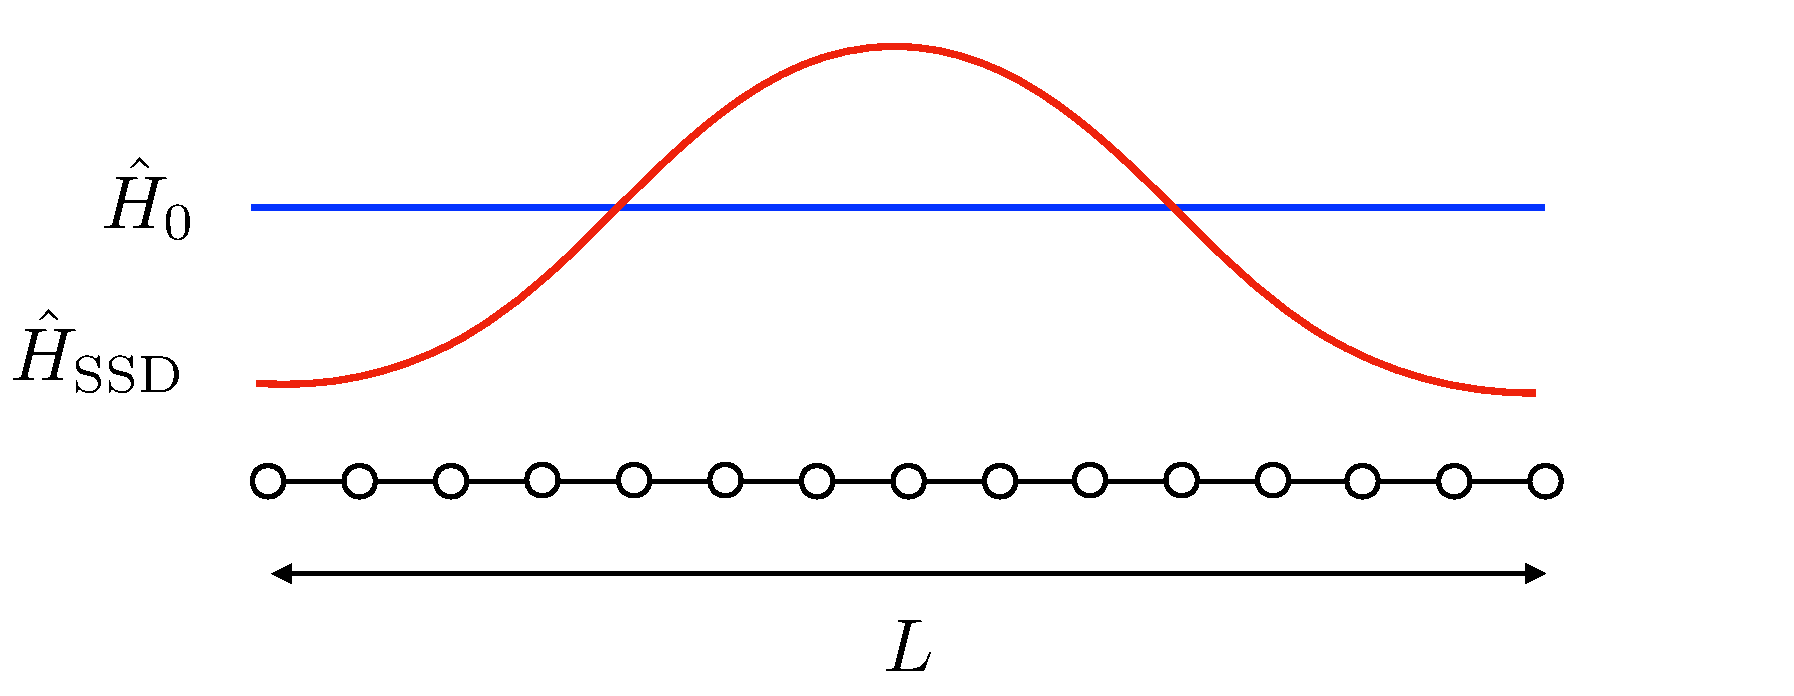
\includegraphics[width=\textwidth]{Floquet_Drive1D_Deformation.pdf}
			\caption{}
		\end{subfigure}
		\begin{subfigure}[b]{0.45\textwidth}
			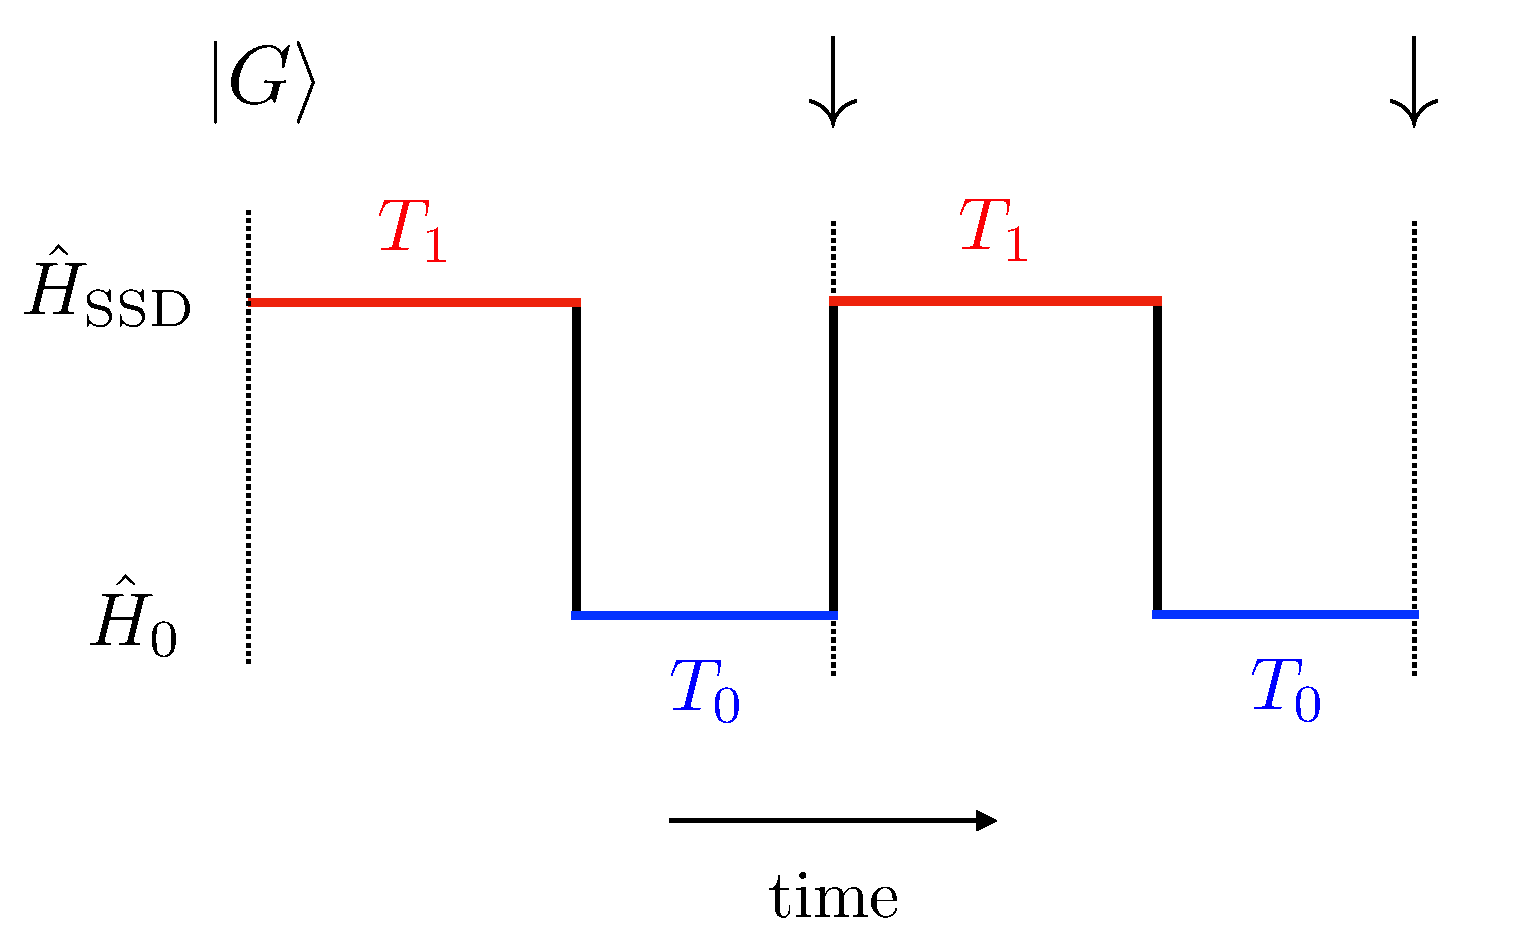
\includegraphics[width=0.95\textwidth]{Floquet_Drive.pdf}
			\caption{}
		\end{subfigure}
		\caption{(a) Hamilton densities for the tight-binding Hamiltonian and SSD deformation (b) Floquet driving where the black arrow indicate stroboscopic measurement}
\end{figure}


\begin{figure}[h]
\centering
		\begin{subfigure}[b]{0.31\textwidth}
			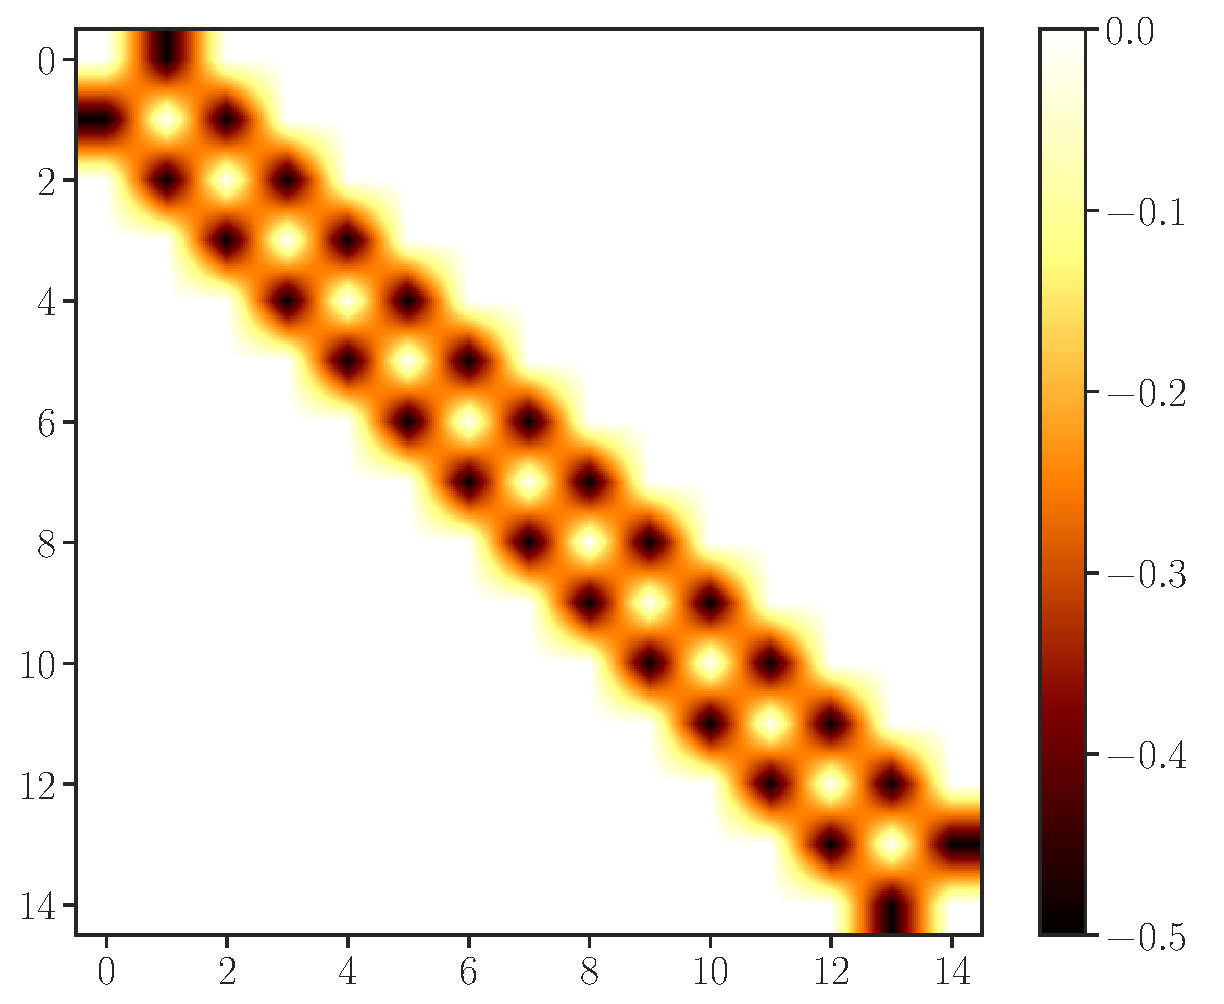
\includegraphics[width=\textwidth]{ColorMapMatrices_OBC}
			\caption{}
		\end{subfigure}
		\begin{subfigure}[b]{0.31\textwidth}
			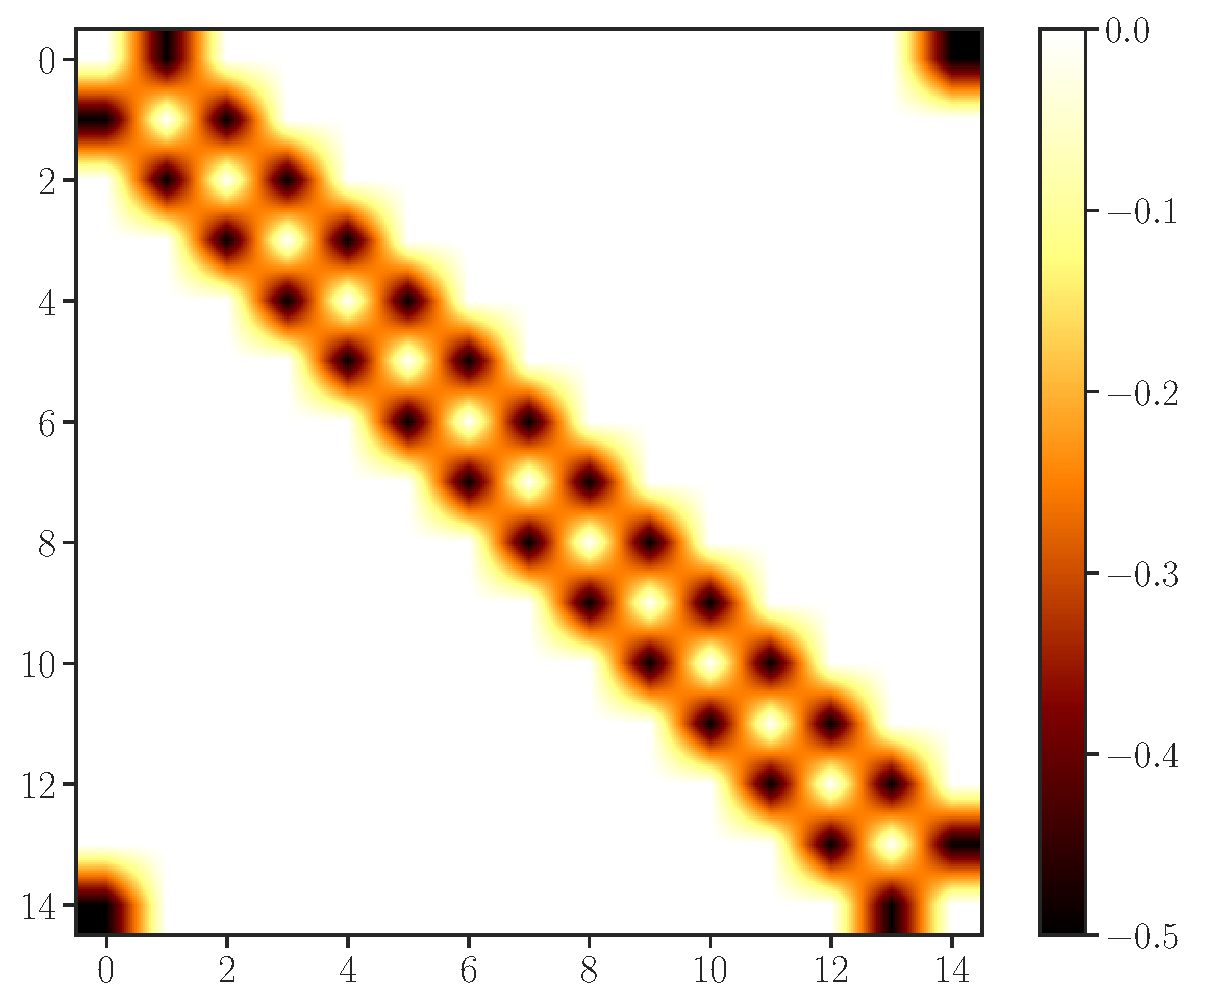
\includegraphics[width=\textwidth]{ColorMapMatrices_PBC}
			\caption{}
		\end{subfigure}
		\begin{subfigure}[b]{0.31\textwidth}
			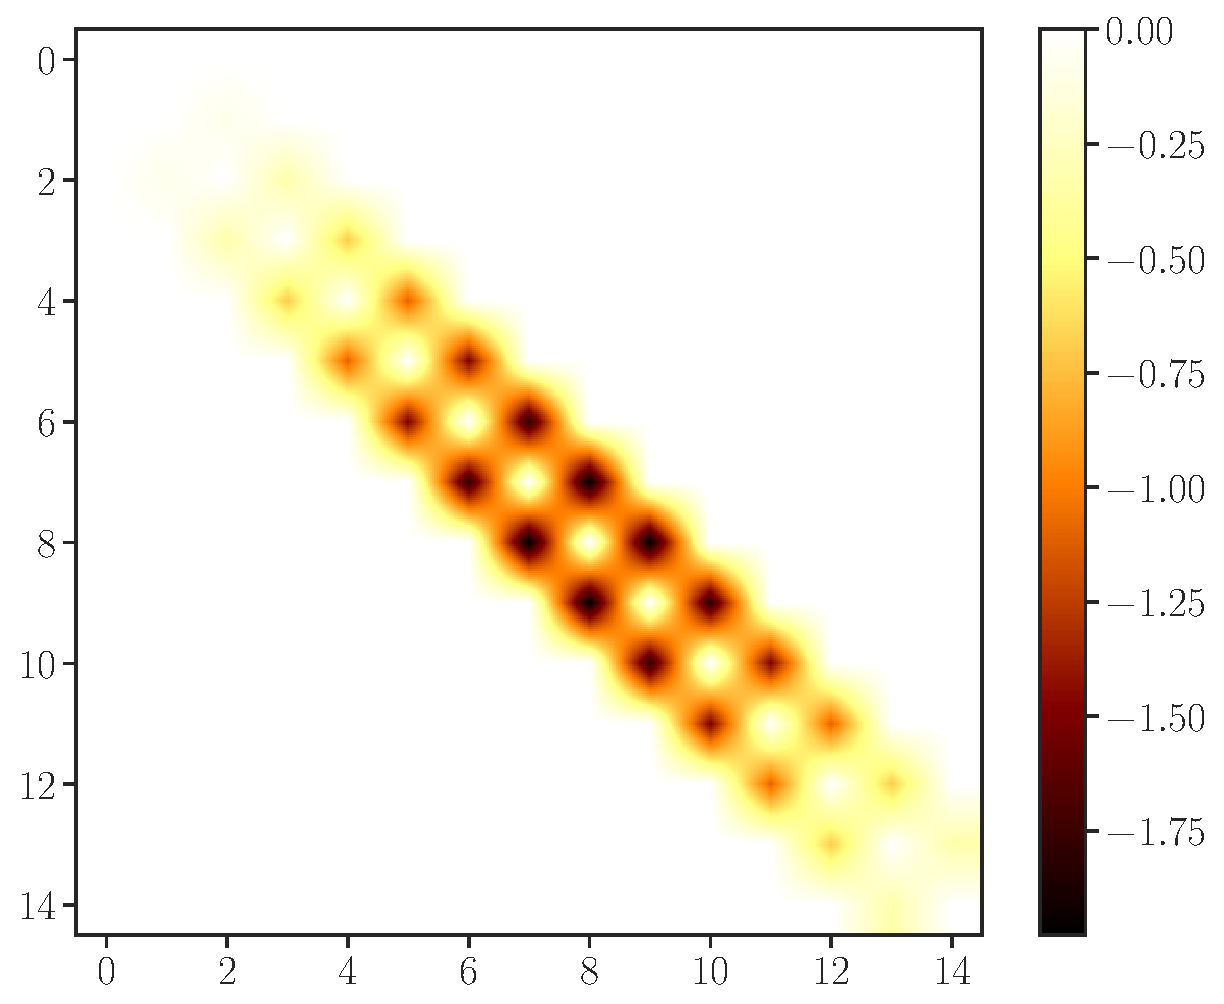
\includegraphics[width = \textwidth]{ColorMapMatrix_SSD}	
			\caption{}
		\end{subfigure}
		\caption{Structure of the tight-binding Hamiltonian for $L = 15$ and (a) open-boundary conditions (b) periodic-boundary conditions (c) sine-squared deformed.}
\end{figure}



%\begin{figure}[h]
%    \centering
%    \subfigure[]{\includegraphics[width=0.24\textwidth]{ColorMapMatrix_PBC}} 
%    \subfigure[]{\includegraphics[width=0.24\textwidth]{ColorMapMatrix_OBC}} 
%    \subfigure[]{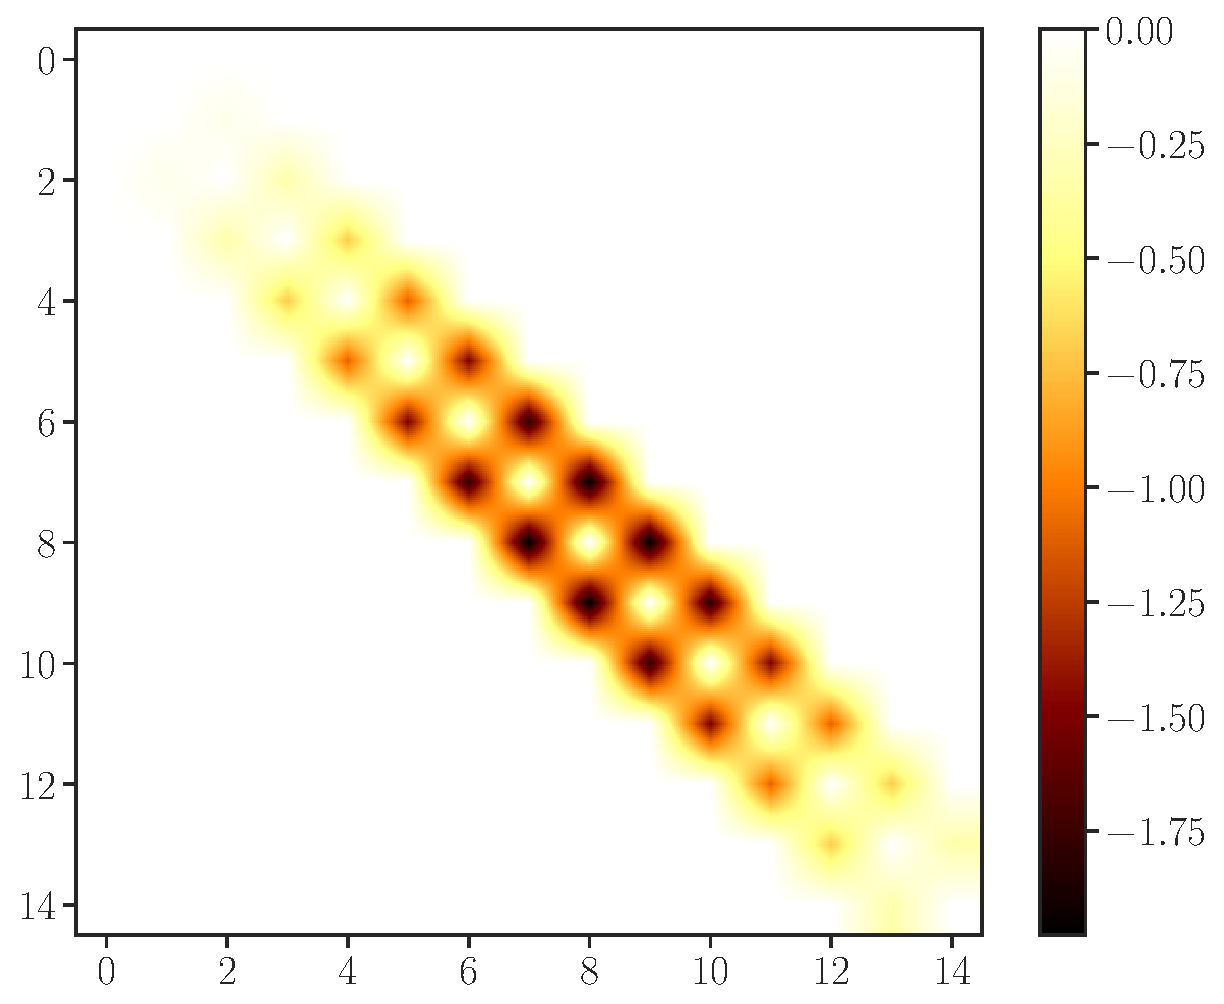
\includegraphics[width=0.24\textwidth]{ColorMapMatrix_SSD}}
%    \caption{(a) blah (b) blah (c) blah (d) blah}
%    \label{fig:foobar}
%\end{figure}

%\begin{figure}[H]
%   \subfloat[\label{genworkflow}]{%
%      \includegraphics[trim=20 40 50 30,clip, width=0.3\textwidth]{ColorMapMatrix_PBC}}
%\hspace{\fill}
%   \subfloat[\label{pyramidprocess} ]{%
%      \includegraphics[trim=10 40 10 30,clip, width=0.3\textwidth]{ColorMapMatrix_OBC}}
%\hspace{\fill}
%   \subfloat[\label{mt-simtask}]{%
%      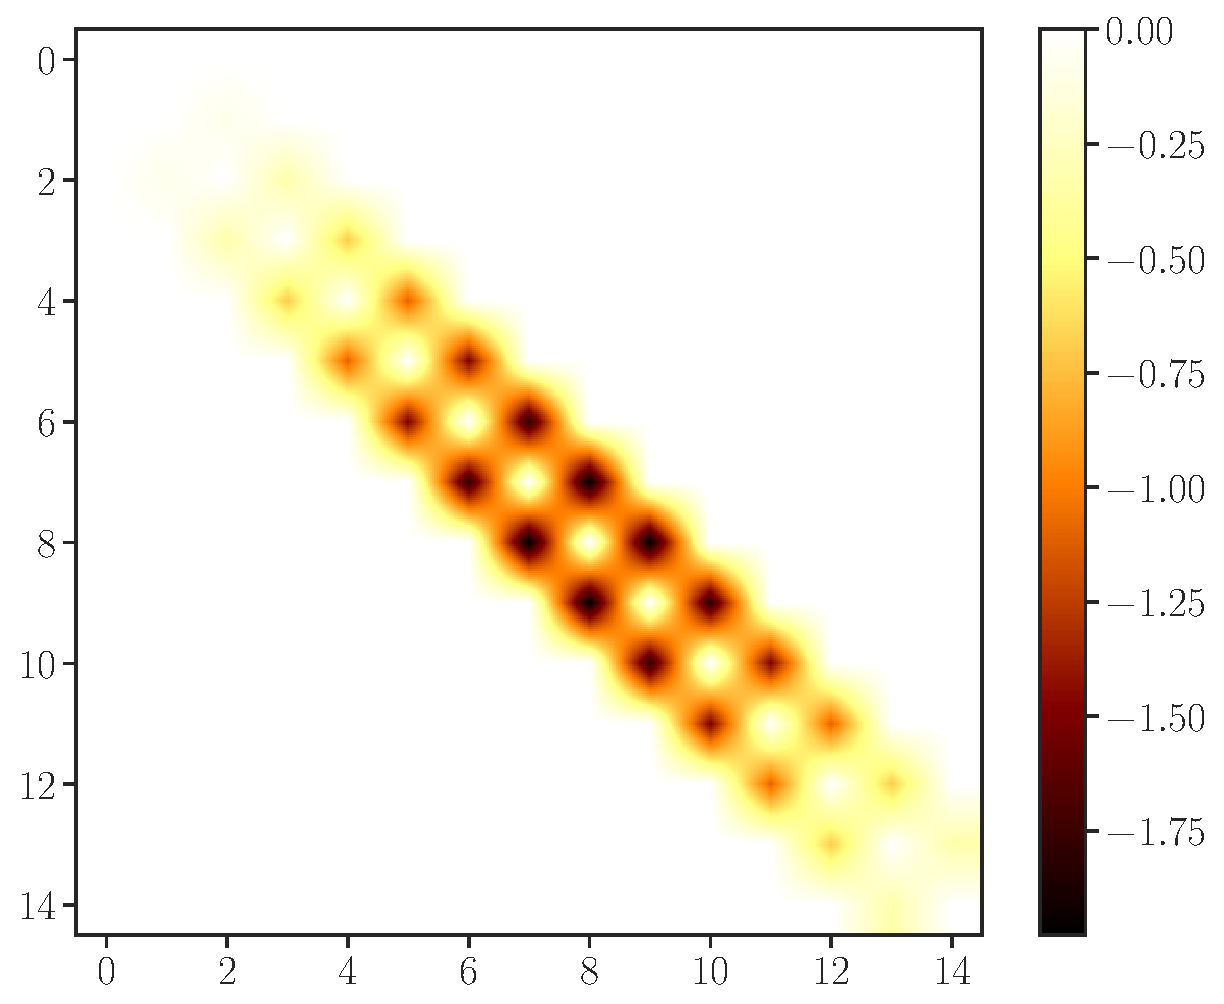
\includegraphics[trim=30 40 30 30,clip, width=0.3\textwidth]{ColorMapMatrix_SSD}}\\
%\caption{\label{workflow}The overall approach. (a) figa; (b) Workflow for figb; (c) Workflow for figc.}
%\end{figure}

%\begin{figure}
%	\centering
%	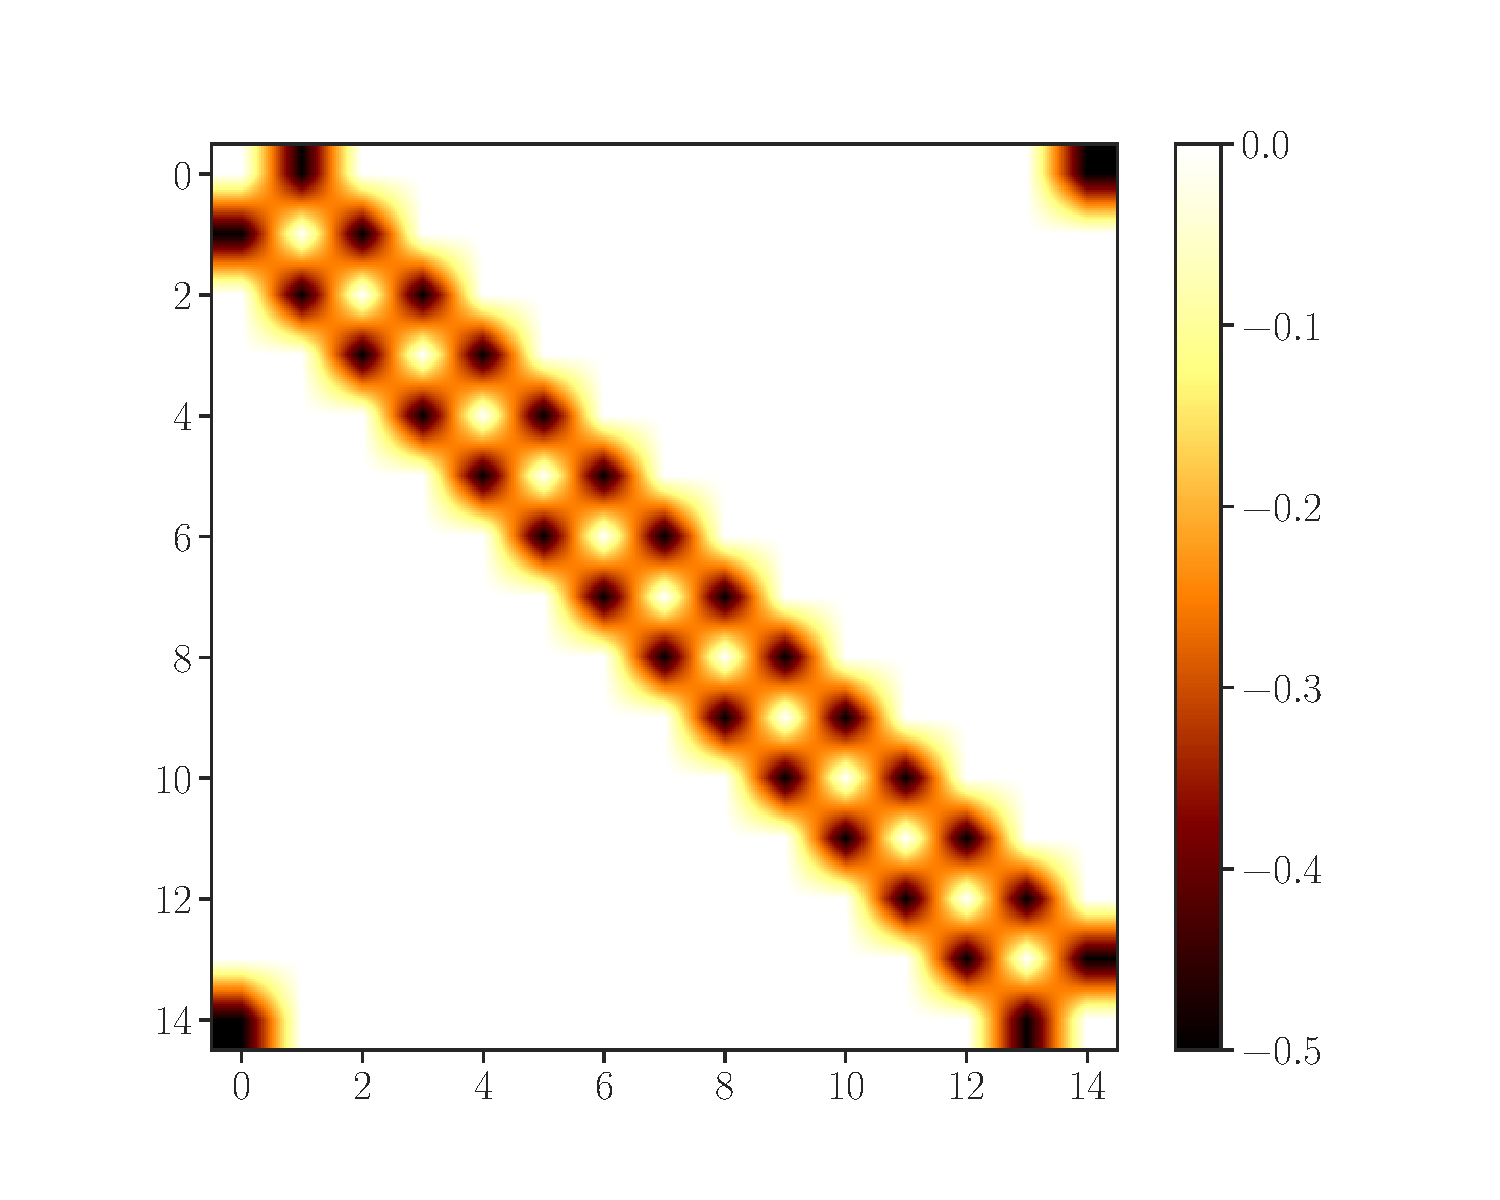
\includegraphics[width = 0.8\textwidth]{ColorMapMatrixH0_PBC}
%\end{figure}

\section{Quantum Quench}

%\begin{figure}[h]
%	\centering
%	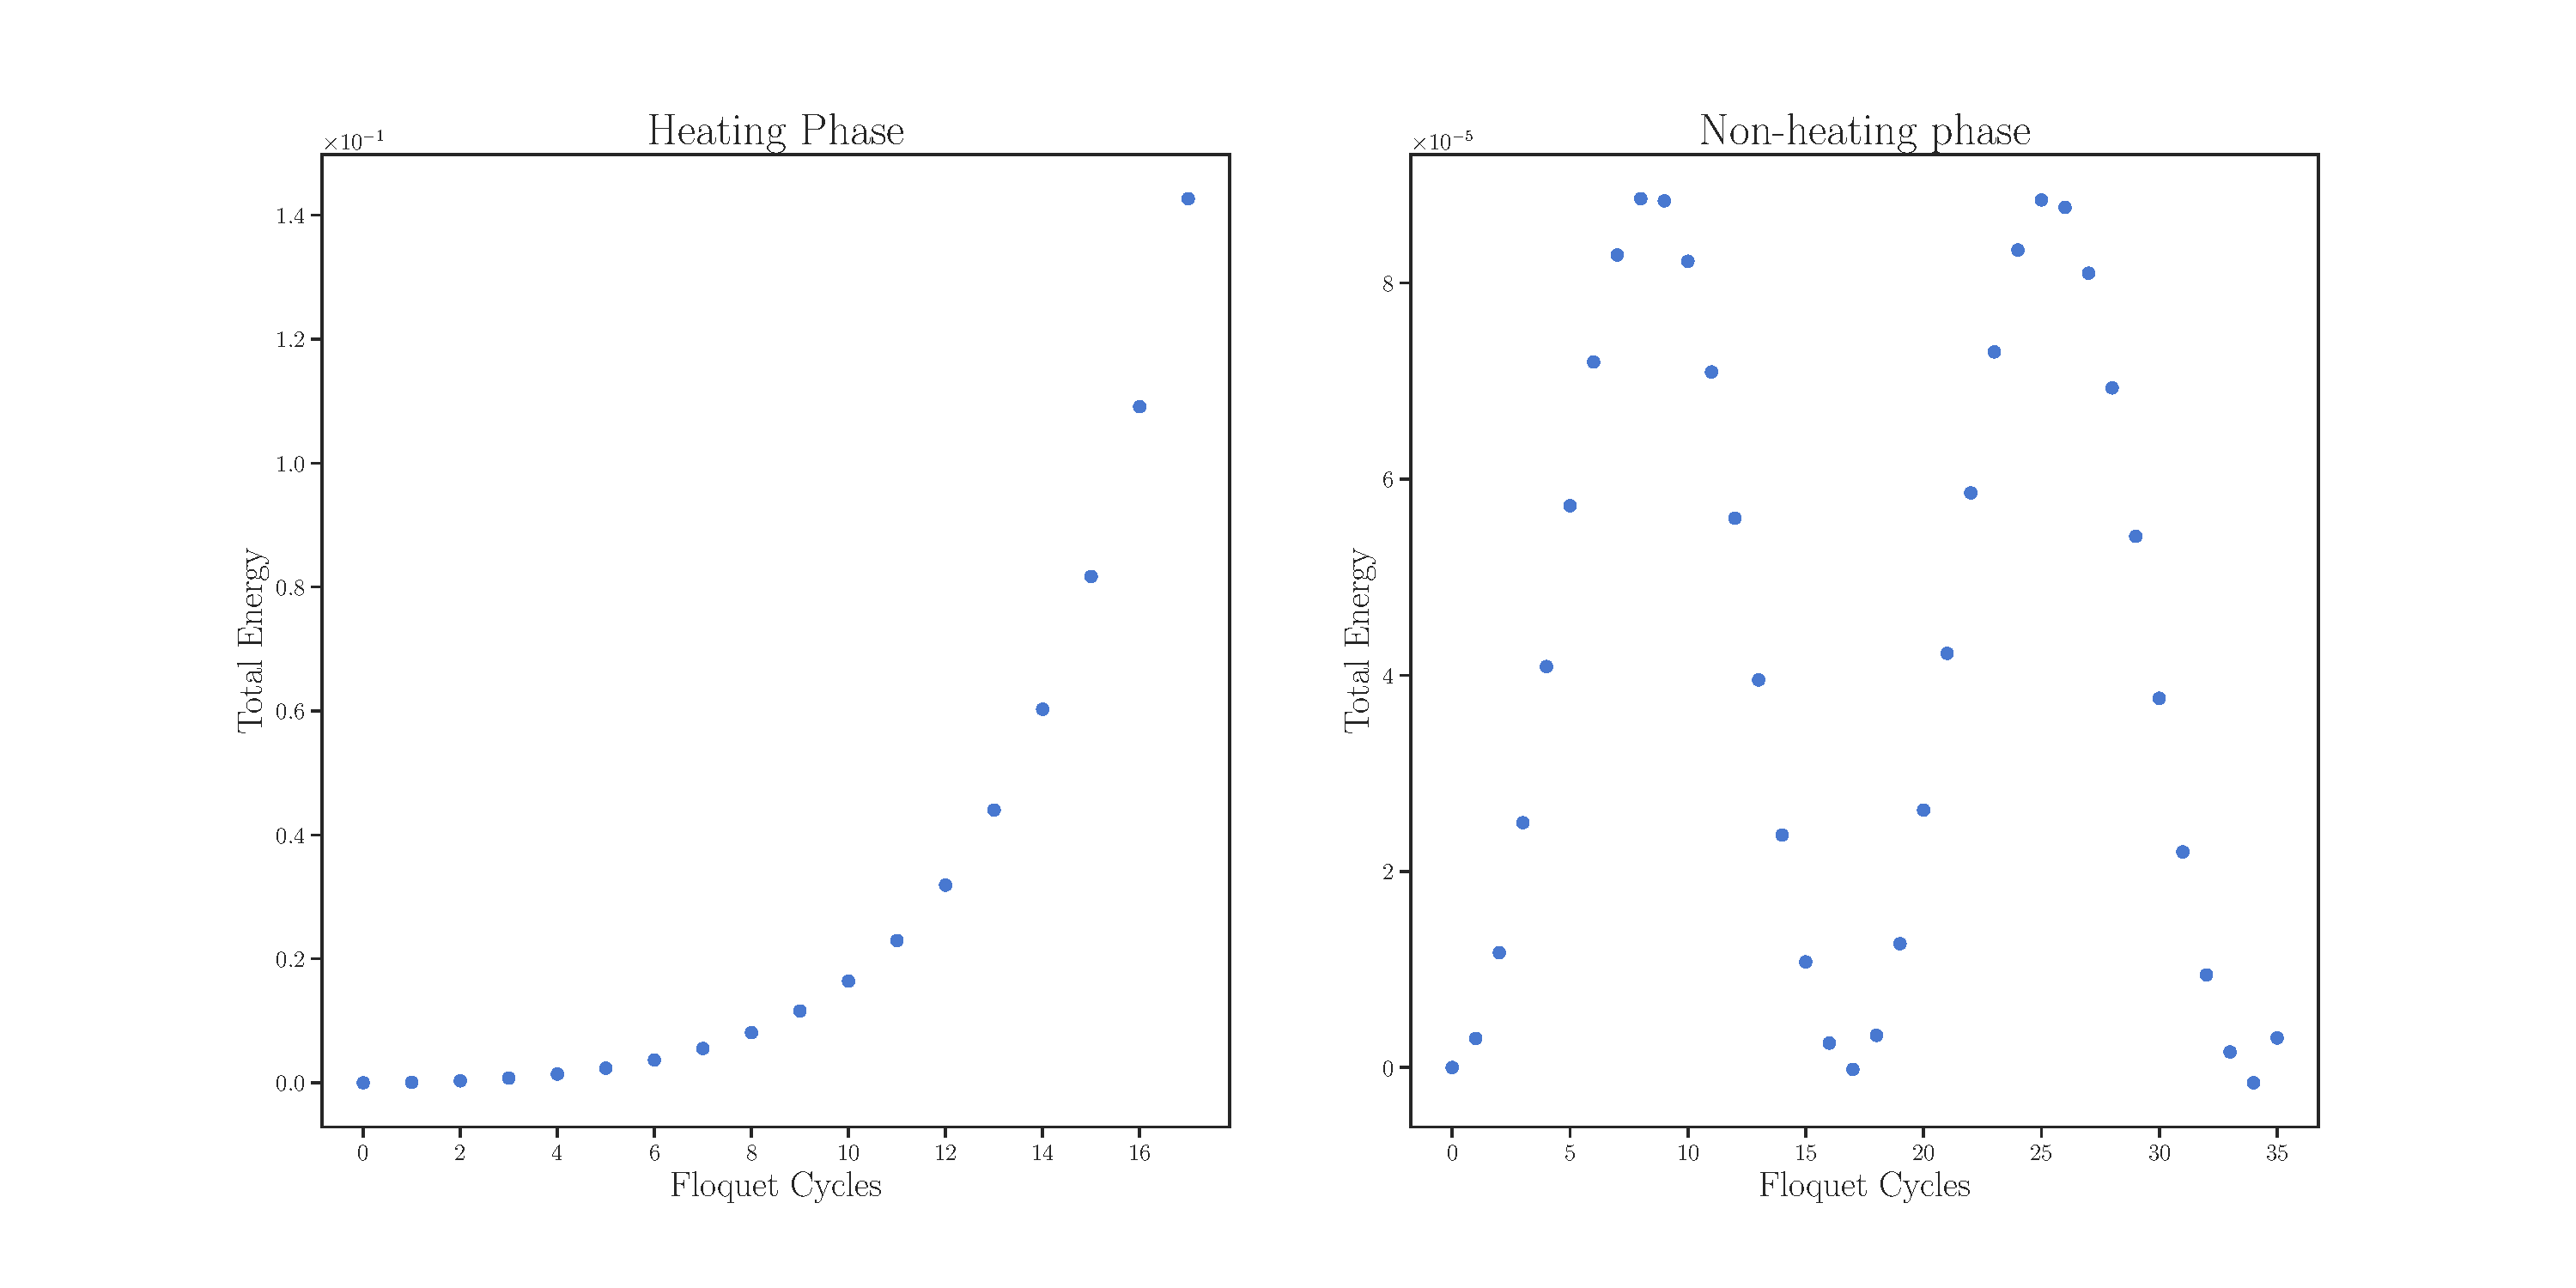
\includegraphics[width=1\textwidth]{Total_Energy1d}
%\end{figure}




\section{Floquet System}

We will consider a free fermion chain with half filling. Our time-dependent Floquet Hamiltonian will be:
	\begin{equation}
	\hat{H}(t) = 
		\begin{dcases}
		\hat{H}_0 = \frac{1}{2} \sum_{i=1}^{L-1} (\hat{c}_i^\dagger \hat{c}_{i+1} + \hat{c}_{i+1}^\dagger \hat{c}_{i})\\
		\hat{H}_\text{SSD} = \sum_{i=1}^{L-1} \sin^2\left( \frac{\pi(i + 1/2)}{L}\right) \left[ \hat{c}_i^\dagger c_{i+1} + \hat{c}_{i+1}^\dagger \hat{c}_i \right]
		\end{dcases}
	\end{equation}

Our aim will be to compute the correlation function $\mel{\psi(t)}{\hat{c}_m^\dagger \hat{c}_n}{\psi(t)}$



\begin{figure}[h]
\centering
\begin{subfigure}[t]{0.49\textwidth}
	\centering
	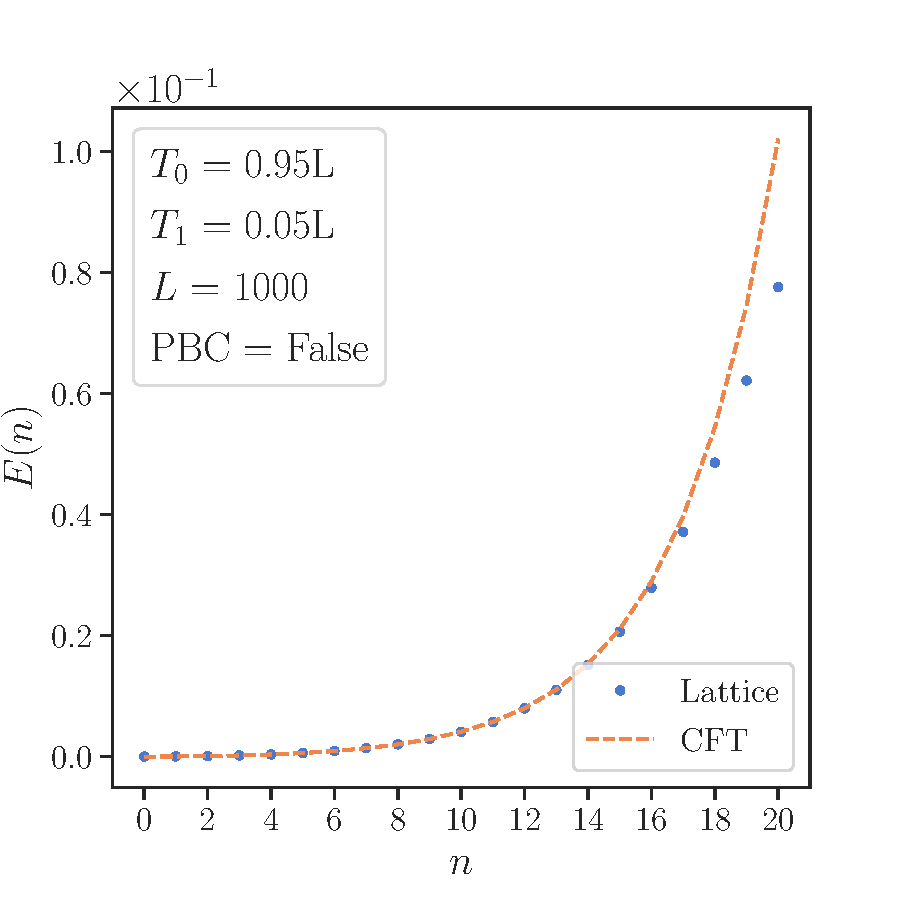
\includegraphics[width =\textwidth]{TotalEnergyHeating}\end{subfigure}
\begin{subfigure}[t]{0.49\textwidth}
	\centering
	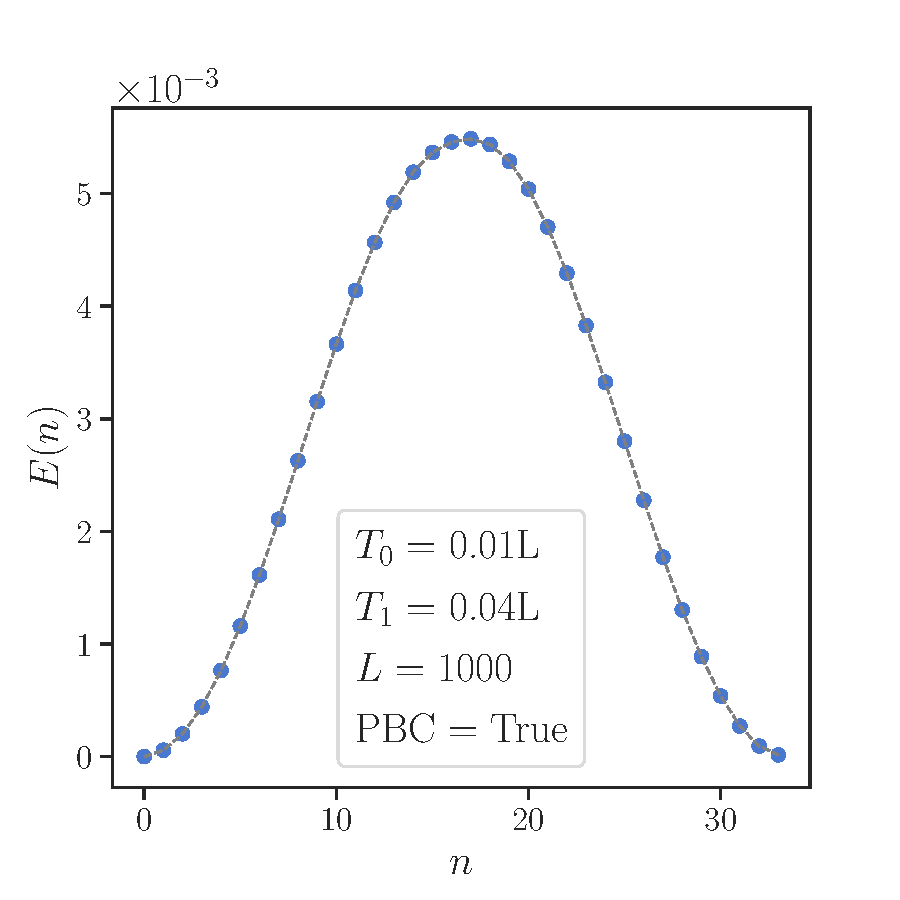
\includegraphics[width =\textwidth]{TotalEnergyNonHeating}
\end{subfigure}
\caption{Evolution of total energy $E(n)$ of a (left) heating phase (right) non-heating phase with respect to the number of cycles $n$.}
\end{figure}



\begin{figure}[h]
	\centering
	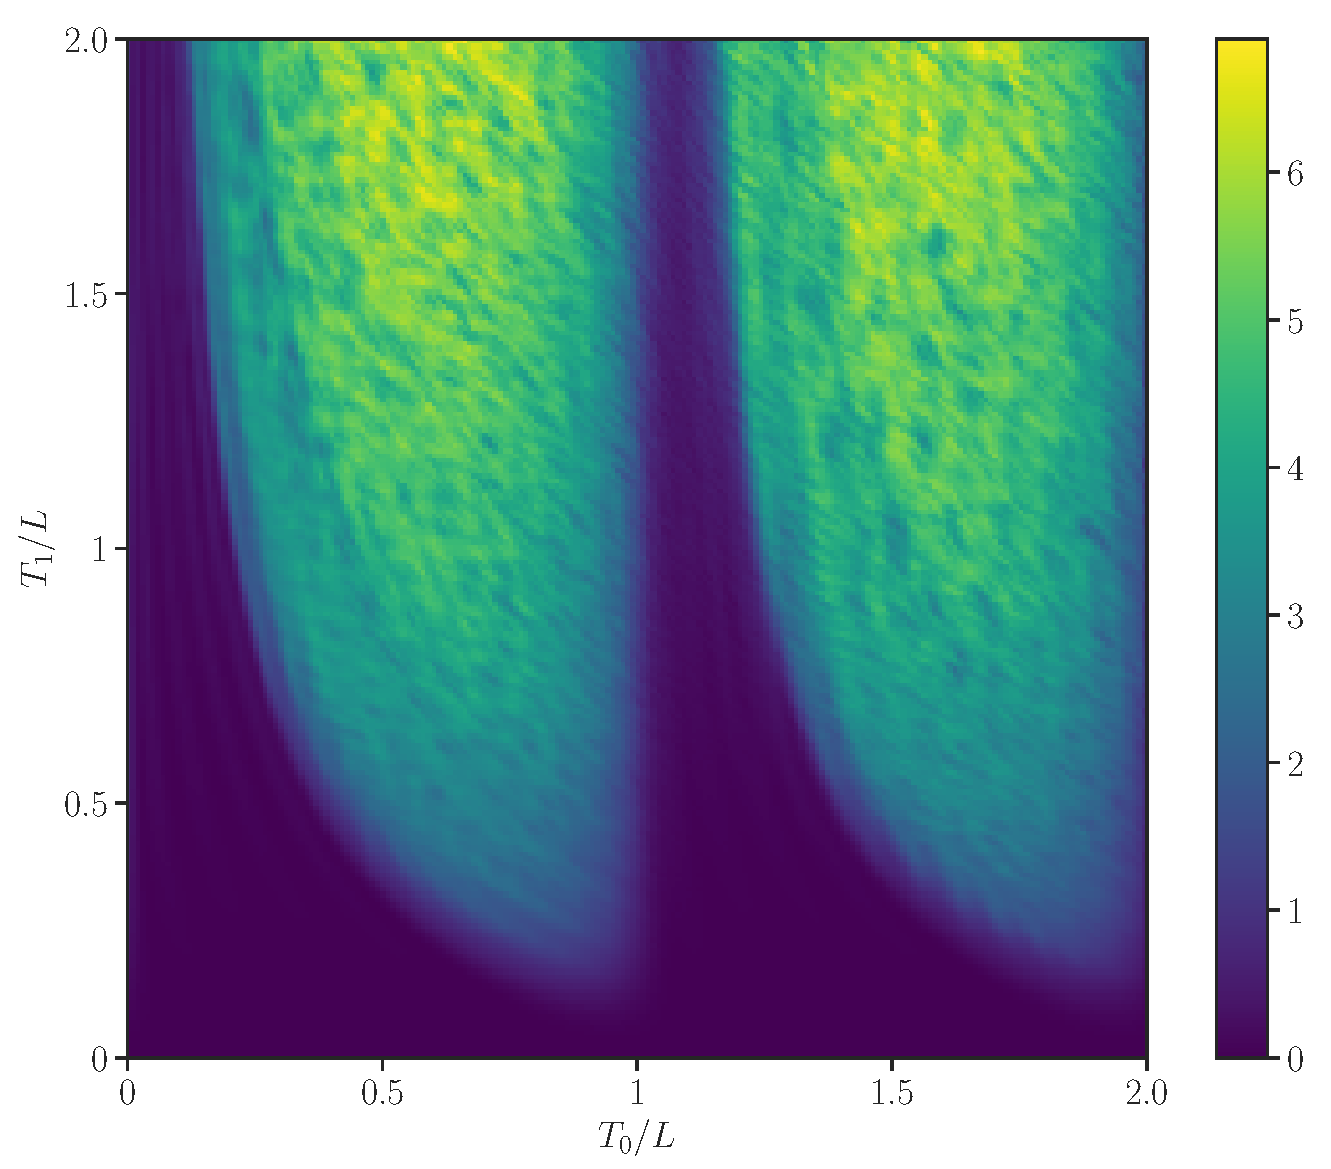
\includegraphics[width=0.8\textwidth]{PhaseDiagram}
	\caption{The Total Energy for a 6-cycle Floquet driven one-dimensional system of $L = 100$ sites as a function of the the two different driving periods $T_0$ and $T_1$. The two different phases are clearly visible and are what we expect to obtain from the Floquet conformal field theory.}
\end{figure}

\subsection{Ground state}





\subsection{Generalization to $n$-cycles}

\section{The quasi-particle picture}
To provide an understanding for the formation of the two energy peaks one can aim to try to describe the evolution with the help of quasi-particles. The velocity of the quasi-particles at the beginning of each cycle is given by the sine-square envelope:
\begin{equation}
	v(x_i) = 2\sin^2(\pi x_i/L)
\end{equation}
since the operator products $\hat{c}_i \hat{c}_{i+1}$ and its adjoint represent kinetic terms.


\section{Theoretical Framework}
	The main goal of this thesis was to establish the entanglement entropy and Energy density of a free fermion lattice under Floquet driving. As we will explicitly show these two quantities can be evaluated with the help of the equal time two-point correlation functions.

	\subsection{Ground State}
	To obtain the matrix form of the Hamiltonian operator $\hat{H}_0$ in the ground state we need to evaluate the correlation matrix
	\begin{equation}
		\mel{G}{\hat{H}_0}{G}
	\end{equation}
	In general this resulting matrix is not diagonal. Our goal is to find a Basistransformation of the creation- and annihiliation operators $\hat{c}$ that will diagonalise $\hat{H}_0$, i.e
	\begin{equation}
		\hat{H}_0 = \sum_{i=1}^L E_i^{(0)} \hat{a}_i^\dagger \hat{a}_i
	\end{equation}
	where the operators once again fullfill the fermionic anticommutation rules
	\begin{equation}
		\{ \hat{a}_i,\hat{a}_j^\dagger \} = \delta_{ij} \qq{and} \{\hat{a}_i^\dagger, \hat{a}_j^\dagger\} = \{\hat{a}_i,\hat{a}_j  \} =0
	\end{equation}
	It is know that a general one-particle operator in second quantized form takes the shape
	\begin{equation}
		\hat{A} = \sum_{\mu, \nu} \mel{\nu}{\hat{A}}{\mu} \hat{a}_\nu^\dagger \hat{a}_\mu
	\end{equation}
	meaning for our Operator in the Ground state we have to evaluate
	\begin{equation}
		\hat{H}_0 = \sum_{n, m} \mel{m}{\hat{H}_0}{n} \hat{c}_m^\dagger \hat{c}_n
	\end{equation}
	Our Goal is it to find an orthogonal matrix representation of this operator. For this note that if $H_{mn} = \mel{m}{\hat{H}_0}{n} = E_n^{(0)} \delta_{mn} $ with the energy-eigenstates $E_n^{(0)}$ of the Hamiltonoperator $\hat{H}_0$ we obtain the diagonal matrix form
	\begin{equation}
	\hat{H} = 
	\begin{pmatrix}
 		\mel{1}{\hat{H}_0}{1} & \mel{1}{\hat{H}_0}{2} & \dots & \mel{1}{\hat{H}_0}{L} \\
 		\mel{2}{\hat{H}}{1} & \ddots &\dots \\
 		\vdots & \dots & \ddots & \vdots \\
 		\mel{L}{\hat{H}}{1}
 	\end{pmatrix}
	\end{equation}
	Our goal is therefore to evaluate the following expressions
	\begin{equation}
		H_{mn} = \mel{\varphi_m}{\hat{H}_0}{\varphi_n} = \mel{0}{\hat{c}_m\hat{H}_0 \hat{c}_n}{0}
	\end{equation}
	where we used the single-particle Basisstates $\{\varphi_m\}$ and the fact that for fermions we can only occupy one particle for each state.
	Inserting the expression for our Hamiltonoperator 
	\begin{equation}
		\hat{H}_0 = \frac{1}{2} \sum_{i=1}^{L-1} \hat{c}_i^\dagger \hat{c}_{i+1} + \hat{c}_{i+1}^\dagger \hat{c}_{i} 
	\end{equation}
	we get
	\begin{align}
	H_{mn}^{(0)} = \frac{1}{2}\sum_{i=1}^{L-1}\mel{0}{\hat{c}_m \left[ \hat{c}_i^\dagger \hat{c}_{i+1} + \hat{c}_{i+1}^\dagger \hat{c}_i\right]\hat{c}_n^\dagger}{0} = \frac{1}{2}\sum_{i=1}^{L-1} \mel{0}{\hat{c}_m \hat{c}_i^\dagger \hat{c}_{i+1} \hat{c}_n^\dagger}{0} + \mel{0}{\hat{c}_m \hat{c}_{i+1}^\dagger \hat{c}_i\hat{c}_n^\dagger}{0}
	\label{eq:Energy_Density_Matrix}
	\end{align}

	
	 However it is known that with a unitary similarity transformation we can reduce it into a diagonal form. For the two terms it follows from Wick's theorem that with the help of contractions we can express any expectation value of Matrix element in terms of the action on the vacuum state $\ket{0}$:
	 \begin{itemize}
	 	\item For the first term in the expression, we obtain
	 	\begin{align}
	 		\sum_i \mel{0}{\hat{c}_m \hat{c}_{i}^\dagger \hat{c}_{i+1} \hat{c}_n^\dagger}{0} &= \sum_i \mel{0}{\hat{c}_m \hat{c}_i^\dagger (\delta_{i +1, n} - \hat{c}_n^\dagger\hat{c}_{i+1})}{0}\\
	 		 &= \sum_i \delta_{i+1, n} \mel{0}{\hat{c}_m \hat{c}_i^\dagger}{0} - \mel{0}{\hat{c}_m \hat{c}_i^\dagger \hat{c}_n^\dagger\hat{c}_{i+1}}{0}
	 		 \label{eq:secondterm2}
	 	\end{align}
	 	where in the second step we used the anticommutator relation for the creation and annihilation operators:
	 	\begin{equation}
	 		\{ \hat{c}_{i+1}, \hat{c}_n^\dagger \} = \hat{c}_{i+1} \hat{c}_n^\dagger + \hat{c}_n^\dagger\hat{c}_{i+1} \; \Rightarrow \; \hat{c}_{i+1} \hat{c}_n^\dagger = \underbrace{\{ \hat{c}_{i+1}, \hat{c}_n^\dagger \}}_{\delta_{i+1, n}} - \hat{c}_n^\dagger \hat{c}_{i+1}
	 		\label{eq:Kommutatorrelation_umgeformt}
	 	\end{equation}
	 	Noting that the second term in (\ref{eq:secondterm2}) is zero due to $\hat{c}_{i+1}\ket{0} =0$ and that with
	 	\begin{equation}
	 		\hat{c}_m \hat{c}_{i}^\dagger = \underbrace{\{ \hat{c}_m, \hat{c}_i^\dagger\}}_{\delta_{m, i}} - \hat{c}_i^\dagger \hat{c}_m
	 	\end{equation}
	 	in analogy to (\ref{eq:Kommutatorrelation_umgeformt}) we finally obtain the expression
	 	\begin{equation}
	 		\mel{0}{\hat{c}_m \hat{c}_i^\dagger \hat{c}_{i+1}\hat{c}_n^\dagger}{0} = \sum_i \delta_{i+1,n}\delta_{m, i} =\delta_{m, n-1}
	 		\label{eq:first_term_correlation_matrix}
	 	\end{equation}
	 	where we again used $\hat{c}_m \ket{0} = 0$ meaning $\mel{0}{\hat{c}_i^\dagger \hat{c}_m}{0} = 0$.
	 	 \item For the second term in the expression, we proceed analogously to above. For completeness, the steps are listed here:
	 	 \begin{align}
	 		\sum_i \mel{0}{\hat{c}_m \hat{c}_{i+1}^\dagger \hat{c}_{i} \hat{c}_n^\dagger}{0} &= \sum_i \mel{0}{\hat{c}_m \hat{c}_{i+1}^\dagger \left( \delta_{i,n} - \hat{c}_n^\dagger \hat{c}_i \right)}{0} \\
	 		&=  \sum_i \delta_{i,n}\mel{0}{\hat{c}_m \hat{c}_{i+1}^\dagger }{0} - \underbrace{\mel{0}{\hat{c}_m \hat{c}_{i+1}^\dagger \hat{c}_n^\dagger\hat{c}_{i+1}}{0}}_{=0}
	 	\end{align}
	 	Using $\hat{c}_m \hat{c}_{i+1}^\dagger = \delta_{m, i+1} - \hat{c}_{i+1}^\dagger \hat{c}_m$ and the fact that $\mel{0}{\hat{c}_{i+1}^\dagger \hat{c}_m}{0} = 0$ we obtain
	 	\begin{equation}
	 		\sum_i \mel{0}{\hat{c}_m \hat{c}_{i+1}^\dagger \hat{c}_i \hat{c}_n^\dagger}{0} = \sum_{i} \delta_{i,n} \delta_{m, i+1} = \delta_{m, n+1}
	 		\label{eq:second_term_correlation_matrix}
	 	\end{equation}
	 \end{itemize}
	 With (\ref{eq:second_term_correlation_matrix}) and (\ref{eq:first_term_correlation_matrix}), it follows that our Hamiltonoperator $\hat{H}_0$ we obtain the bi-diagonal form:
	 \begin{equation}
	 	H^{(0)}_{mn} = \frac{1}{2} \left(\delta_{m, n+1} + \delta_{m+1, n}\right)
	 \end{equation}
	 It can analogously be shown, that for the Hamiltonian $\hat{H}_1$ we obtain following Matrixelements
	 \begin{equation}
	 	H_{mn}^{(\text{SSD})} = \sin^2\left(\frac{\pi(n-1/2)}{L}\right) \delta_{m,n-1} + \sin^2\left(\frac{\pi(n+1/2)}{L}\right) \delta_{m,n}
	 \end{equation}
	 It is clear that the two-point Correlation Matrix is not diagonal in the single-particle Basis set $\{ \varphi_i \}$. To diagonalize the matrix we consider a change of basis to some other single-particle basis set $\{\psi_j\}$ with
	 \begin{equation}
	 	\hat{a}_j = \sum_i \braket{\psi_j}{\varphi_i} \hat{c}_i \qq{and} \hat{a}_j^\dagger =\sum_i \braket{\varphi_i}{\psi_j} \hat{c}_i^\dagger
	 \end{equation}
	 If we let $U_{i,j} = \braket{\varphi_i}{\psi_j}$ be the matrix elements of the unitary transformation we can compactly write
	 \begin{equation}
	 	\hat{a}_j = \sum_i (U^\dagger)_{ji} \hat{c}_i \qq{and} \hat{a}_j^\dagger = \sum_i (U^\dagger)^*_{ji} \hat{c}_i^\dagger =\sum_{i}  \hat{c}_i^\dagger U_{ij}
	 \end{equation}
	 
	 
	 
	 where we used $U_{ij}^* = (U^\dagger)_{ji}$. To show that the transformation matrix is indeed unitary, consider
	 \begin{align}
	 	\delta_{j,k} &= \braket{\psi_j}{\psi_k} = \sum_i \braket{\psi_j}{\varphi_i}\braket{\varphi_i}{\psi_k} = \sum_i \braket{\varphi_i}{\psi_j}^* \braket{\varphi_i}{\psi_k} \\
	 	&= \sum_i U_{ij}^* U_{ik} = \sum_i (U^\dagger)_{ji} U_{ik} = (U^\dagger U)_{jk} \quad \Rightarrow \quad U^\dagger U = \mathbbm{1}
	 \end{align}
	 The inverse of this transformation yields
	 \begin{equation}
	 	\hat{c}_n = \sum_i U_{ni} \hat{a}_i \qq{and} \hat{c}_n^\dagger = \sum_i \hat{a}_i^\dagger U^*_{ni} = \sum_i \hat {a}_i^\dagger (U^\dagger)_{in}
	 \end{equation}
	 It is well known that any hermitian matrix $A$ is diagonalizable by an appropriate unitary similarity transformation
	 \begin{equation}
	 	U^\dagger A U = \begin{pmatrix}
	 		\lambda_1 & 0 &\dots & 0 \\
	 		0 & \lambda_2 & \dots & 0 \\
	 		\vdots & \vdots & \ddots & \vdots \\
	 		0 & 0 & \dots & \lambda_n
	 	\end{pmatrix}
	 \end{equation}
	 where $\lambda_1, \dots \lambda_n$ are the eigenvectors of the hermitian matrix $A$ and the columns of $U$ are spanned by the eigenvectors of the hermitian matrix $A$. By this given unitary transformation we can diagonalise the Hamiltonian:
	 \begin{equation}
	 	\hat{H}_0 = \sum_{i=1}^L E_i^{(0)} \gamma_i^\dagger \gamma_i = E_i^{(0)} \hat{n}_i
	 \end{equation}
	 where $\hat{n}_i$ denotes the fermionic occupation number operator at site $i$. In the case of translational invariance for the chain (i.e closed boundary conditions) a simple choice of unitary transformation would be transforming to the momentum basis (essentially using a Fourier transform). We simply want to consider a general case with open- or closed boundary conditions. Since we are considering a half-filled free fermion chain our ground state $\ket{G}$ in these new operators can be written as:
	 \begin{equation}
	 	\ket{\psi(0)} =\ket{G} = \prod_{i=1}^{L/2} \gamma_i^\dagger \ket{0}
	 \end{equation}
	 We note that in the case of periodic boundary conditions the operators $\hat{\gamma}_i, \hat{\gamma}_i^\dagger$ correspond to the operators $\hat{c}_k$ and $\hat{c}_k^\dagger$ respectively.
	 
	 
	\subsection{Electrons filled on the left hand side of the chain}
	
	It can be shown that in this case the correlation matrix will take the form
	\begin{equation}
		\mel{H}{\hat{c}_n^\dagger \hat{c}_m}{H} = \sum_{j=1}^{L/2} (\mathcal{W} U^\dagger)_{nj} (U\mathcal{W}^\dagger)_{jm}
	\end{equation}
	where $\ket{H}$ corresponds to the state with electrons filled from the left hand side of the chain
	\begin{equation}
		\ket{H} = \sum_{j=1}^{L/2} \hat{c}_j^\dagger \ket{0}
	\end{equation}
	

	\subsection{Quantum Quench and Floquet Case}
	This procedure follows closely the paper of Xueda Wen \cite{Xueda} \\
	
	Our goal will be to find the two-point correlation function
	For a single quench 
	After time $T_0$ has passed we now want to consider what happens to a single quench by evolving the ground state $\ket{G}$. Since $\hat{H}_\text{SSD}$ is time-independent it is well know that the time evolution of a state $\ket{\psi(t)}$ in the Schrödinger picture is given by applying the unitary evolution operator $\hat{U} = \exp(i\hat{H}_\text{SSD} t)$ on the ground state $\ket{\psi(t=0)} = \ket{G}$:
	\begin{equation}
		\ket{\psi(t)} = \exp(-i \hat{H}_1 t) \ket{G}
	\end{equation}
	We wish to evaluate the equal-time two-point correlation function:
	\begin{equation}
	\mathcal{C}_{m,n} = \mel{\psi(t)}{\hat{c}_m^\dagger \hat{c}_n}{\psi(t)}	
	\end{equation}
	\begin{equation}
		\mathcal{C}_{\mathcal{O}} = \expval{\hat{\mathcal{O}}} = \text{Tr}(\rho \hat{\mathcal{O}})
	\end{equation}
	The correlation function for our case not in thermale equilibrium is given by
	\begin{equation}
		 = \frac{1}{\operatorname{tr}\left(e^{-\beta H}\right)} \operatorname{tr}\left(c_{i}^{\dagger} c_{j} e^{-\beta H}\right)
	\end{equation}
Instead of working in the Schrödinger picture we want to work in the Heisenberg one. Therefore we consider
	\begin{equation}
		\mel{\psi(t)}{\hat{c}_m^\dagger \hat{c}_n}{\psi(t)} = \mel{G}{e^{i \hat{H}_1 t} \hat{c}_m^\dagger \hat{c}_n e^{-i \hat{H}_1 t}}{G} = \mel{G}{e^{i\hat{H}_1 t} \hat{c}_m^\dagger e^{-i \hat{H}_1 t} e^{i \hat{H}_1 t} \hat{c}_n e^{-i\hat{H}_1 t}}{G}
		\label{eq:Correlation_Matrix_singlequench}
	\end{equation}
	Where in the second equality we inserted the expression $\hat{U}^\dagger \hat{U} = \exp(i \hat{H}_1 t)\exp(-i \hat{H}_1 t) = \mathbbm{1}$. Our goal will be to simply the two expressions:
	\begin{equation}
		\bra{G} e^{i\hat{H}_1 t} \hat{c}_m^\dagger e^{-i \hat{H}_1 t} \qq{and}  e^{i \hat{H}_1 t} \hat{c}_n e^{-i\hat{H}_1 t}\ket{G}
	\end{equation}
	such that the two-point correlation function (\ref{eq:Correlation_Matrix_singlequench}) for a single-quench only depends on the unitary transformation that diagonalize the Hamiltonians $\hat{H}_0$ and $\hat{H}_1$. \\
	
	 To diagonalize the driven Hamiltonian $\hat{H}_1$ consider a unitary basis transformation $V$ that transforms our operators according to
	\begin{equation}
		\hat{b}_j = \sum_i (V^\dagger)_{ji} \hat{c}_i \qq{and} \hat{b}_j^\dagger = \sum_i (V^\dagger)^*_{ji} \hat{c}_i^\dagger =\sum_i \hat{c}_i^\dagger V_{ij}
	\end{equation}
	such that 
	\begin{equation}
		\hat{H}_1 = \sum_i E_i^{(1)} \hat{b}_i^\dagger \hat{b}_i
	\end{equation}
	and 
	\begin{equation}
		\hat{c}_n = \sum_j V_{nj } \hat{b}_j \qq{and} \hat{c}_n^\dagger = \sum_j (V^\dagger)^*_{nj} \hat{b}_j^\dagger = \sum_j \hat{b}_j (V^\dagger)_{jn}
	\end{equation}
	Expressing our operators $\hat{b}_j$ and $\hat{b}_j^\dagger$ in terms of our creation and annihilation operators $\hat{a}_i$ and $\hat{a}_i^\dagger$:
	\begin{align}
		\hat{b}_j &= \sum_i (V^\dagger)_{ji} \hat{c}_i = \sum_i (V^\dagger)_{ji} \sum_k U_{ik} \hat{a}_k = \sum_k (V^\dagger U)_{jk} \hat{a}_k \\
		\hat{b}_j^\dagger &= \sum_i  \hat{c}_i^\dagger V_{ij} = \sum_i \sum_k \hat{a}_k^\dagger (U^\dagger)_{ki} V_{ij} = \sum_k \hat{a}_k (U^\dagger V)_{kj}
	\end{align}
	If we define another Matrix as $W = V^\dagger U$ such that $W^\dagger = U^\dagger V$ we obtain the expression:
	\begin{equation}
		\hat{b}_j = \sum_k W_{jk} \hat{a}_k \qq{and} \hat{b}_j^\dagger = \sum_k \hat{a}_k^\dagger (W^\dagger)_{kj}
		\label{eq:expression_b_j}
	\end{equation}
	From this it follows that
	\begin{align}
		e^{i \hat{H}_1 t} \hat{c}_n e^{-i \hat{H}_1 t} \ket{G} &=  e^{i \hat{H}_1 t} \sum_j V_{nj} \hat{b}_j e^{-i \hat{H}_1 t}\ket{G} 
	\end{align}
	using the fact that $e^{i \hat{H}_1 t} \hat{b}_j e^{-i \hat{H}_1 t} = e^{-i E_j^{(1)} t} \hat{b}_j$ and the expression $\hat{b}_j$ from (\ref{eq:expression_b_j}) we get
	\begin{align}
		\sum_j V_{nj} e^{i \hat{H}_1 t} \hat{b}_j e^{-i\hat{H}_1 t} = \sum_j V_{nj} e^{-i E_j^{(1)}t} \hat{b}_j = \sum_j V_{nj} e^{-i E_j^{(1)} t} \sum_j W_{jk} \hat{a}_k = \sum_j V_{nj} \sum_k W_{jk}^{(t), 1} \hat{a}_k
	\end{align}
	where we additionally defined
	\begin{equation}
		W_{jk}^{(t),1} = e^{-i E_j^{(1)}} W_{jk}
	\end{equation}
	meaning we have
	\begin{equation}
		e^{i \hat{H}_1 t} \hat{c}_n  e^{-i \hat{H}_1 t} \ket{G} = \sum_k [ V\cdot W^{(t), 1}]_{nk} \hat{a}_k
		\label{eq:expression_left_Evolution}
	\end{equation}
	Analogously we can show that
	\begin{equation}
		\bra{G} e^{i \hat{H}_1 t} \hat{c}_m^\dagger e^{-i \hat{H}_1 t} = \sum_{k'}\bra{G} \hat{a}_{k'}^\dagger [V \cdot W^{(t), 1} ]^\dagger_{k',m}
	\end{equation}
	which one can also convince oneself of by simply taking the complex conjugate of equation (\ref{eq:expression_left_Evolution}). Consequently for the two-point correlation function we obtain:
	\begin{equation}
	\begin{split}
	\mel{G}{e^{i \hat{H}_1 t} \hat{c}_m^\dagger e^{-i\hat{H}_1 t} e^{-i \hat{H}_1 t} \hat{c}_n e^{-i \hat{H}_1 t}}{G} &= \mel {G}{\sum_{k'}\hat{a}_{k'}^\dagger [ V \cdot W^{(t),1}]_{k',m}^\dagger \sum_k [V \cdot W^{(t),1 } ]_{nk} \hat{a}_k}{G}\\
	&= \sum_{k \in \text{occ}} [ V \cdot W^{(t),1} ]_{nk} \cdot [V\cdot W^{(t),1} ]_{km}^\dagger
	\end{split}
	\end{equation}
	where in the second step we used that the correlation matrix only does not vanish if $k' = k$ and that $\mel{G}{\hat{a}_k^\dagger \hat{a}_k}{G} = 1$ for all $k$ for which the ground state is occupied.
	
	\subsubsection{Double Quench}
	We now want to state the correlation matrix for a double quench meaning we want to consider the state
	\begin{equation}
		\ket{\psi(t)} = e^{i \hat{H}_0 T_0} e^{i \hat{H}_1 T_1} \ket{G}
	\end{equation}
	where $t = T_0 + T_1$
	
	\subsubsection{Generalization}
	We can essentially see the Generalization as a product of double quenches meaning for the Floquet case of $n$-cycles with $t = n(T_0 + T_1)$
	\begin{equation}
		\ket{\psi(t)} = e^{-i \hat{H}_0 T_0} e^{-i \hat{H}_1 T_1} \dots e^{-i \hat{H}_0. T_0 } e^{-i \hat{H}_1 T_1} \ket{G}
	\end{equation}
	the two point correlation function can simply be computed as a product of the unitary transformation matrices
	\begin{equation}
		\mel{\psi(t)}{\hat{c}_m^\dagger \hat{c}_n }{\psi(t)} = \sum_{k \in \text{occ}} \mathcal{W}_{nk}  \cdot (\mathcal{W}^\dagger)_{km}
	\end{equation}
	with 
	\begin{equation}
		\mathcal{W} = U \cdot [W^{(T_0),0} \cdot W^{(T_1), 1}]^n = U \cdot [ W^{(T_0),0} \cdot W^{(T_1), 1}] \dots [ W^{(T_0), 0} \cdot W^{(T_1), 1}] 
	\end{equation}
	The correlation function therefore implicitly depends on the how many states $k$ in the lattice are occupied. \\
	
	It should be noted that our measurements were taken in a stroboscopic manner, as can also be seen from the used time steps in the expansions


\begin{equation}
	E(n) =\expval*{\hat{H}_0} = \mel{\psi(t)}{\hat{H}_0}{\psi(t)} = \sum_{i=1}^{L-1} \mathcal{C}_{i, i+1} + \mathcal{C}_{i+1, i}
\end{equation}
	

\begin{figure}[h]
\centering
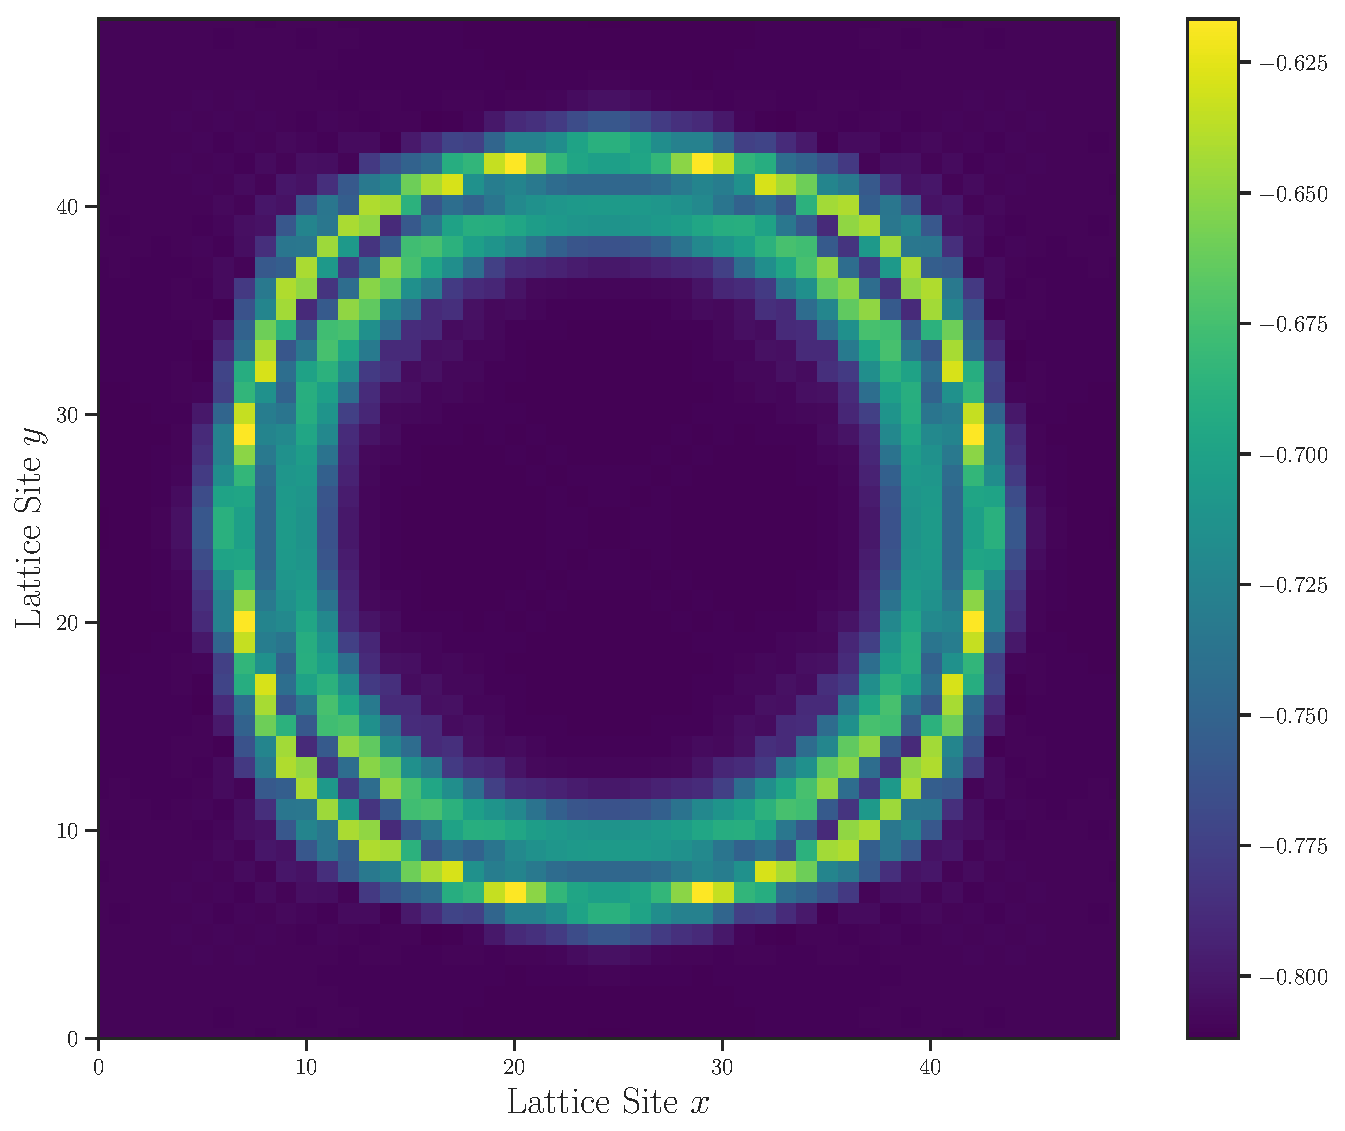
\includegraphics[width=0.8\textwidth]{Energydensity2d_nearest.pdf}	
\caption{Heating phase for the 2D Floquet System after 10 cycles for a system of $L = 50$ Lattice Sites. The parameters here are $T_0 = -0.5L$ and $T_1 = 0.5L$.}
\end{figure}




\section{Floquet System in one dimension}


\begin{figure}[h]
\centering
\begin{subfigure}[t]{0.49\textwidth}
	\centering
	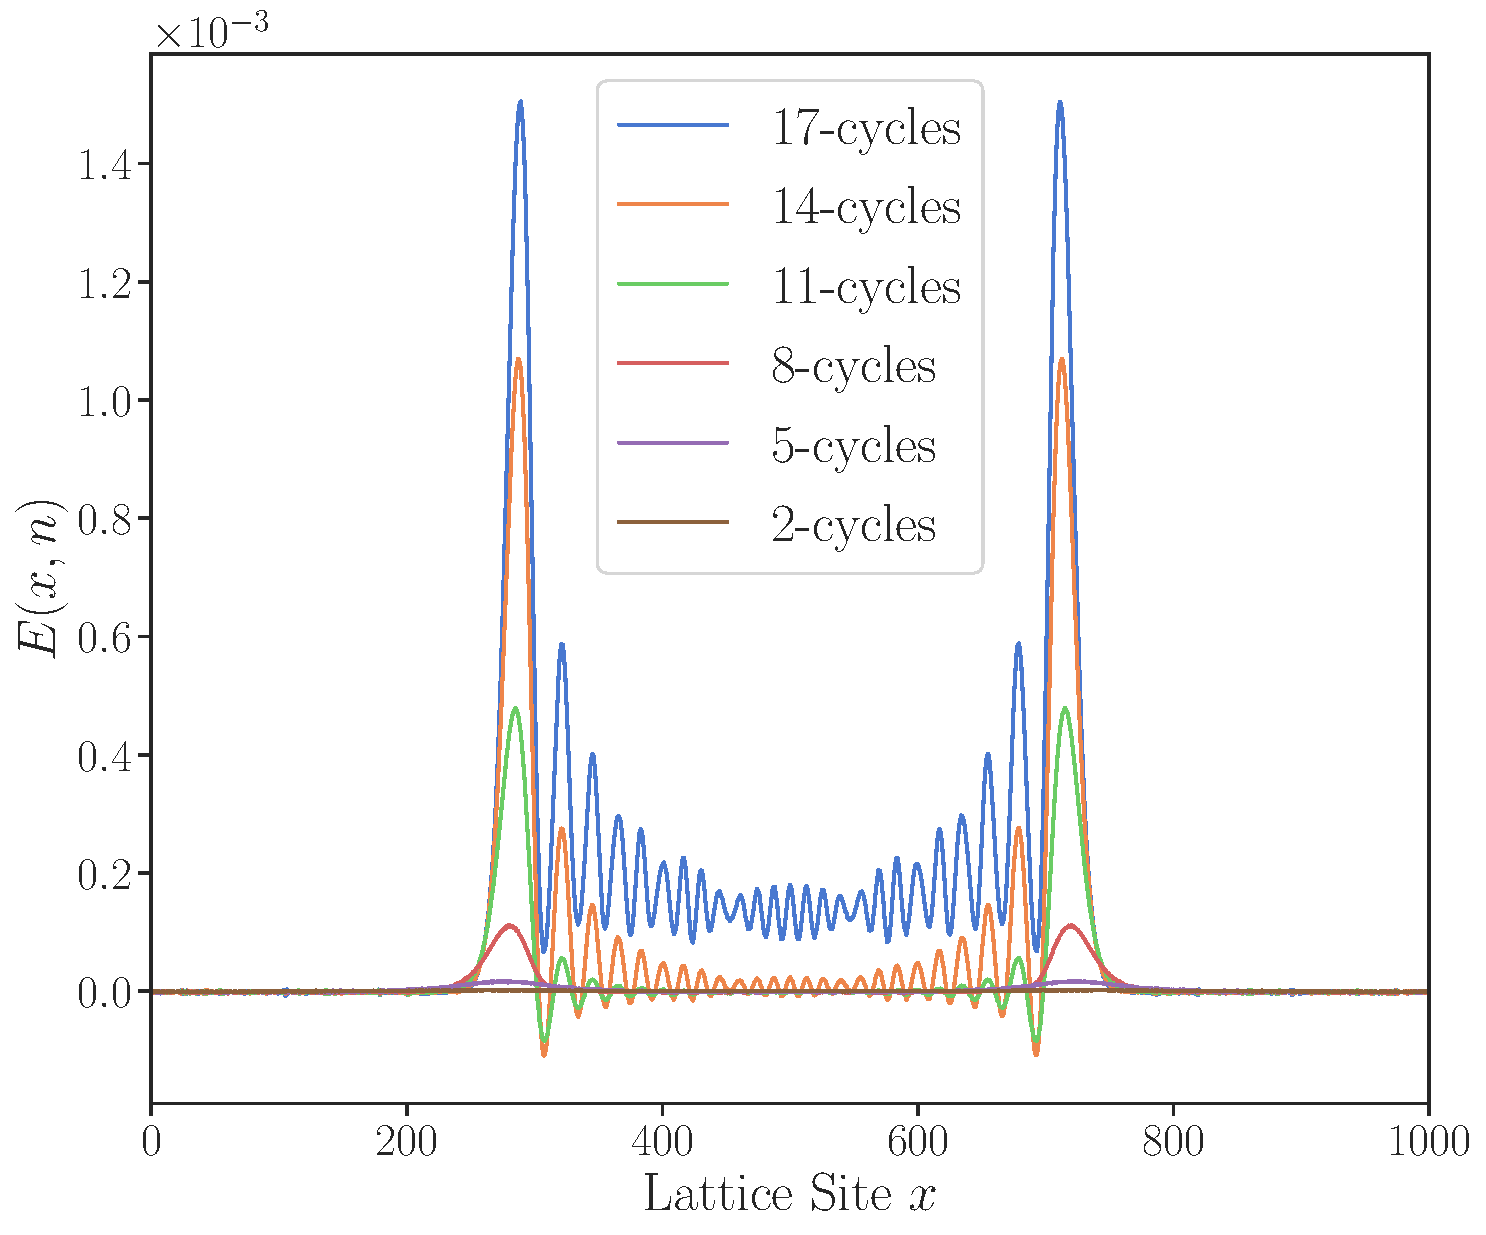
\includegraphics[width =\textwidth]{Energy_Density1}
\end{subfigure}
\begin{subfigure}[t]{0.49\textwidth}
	\centering
	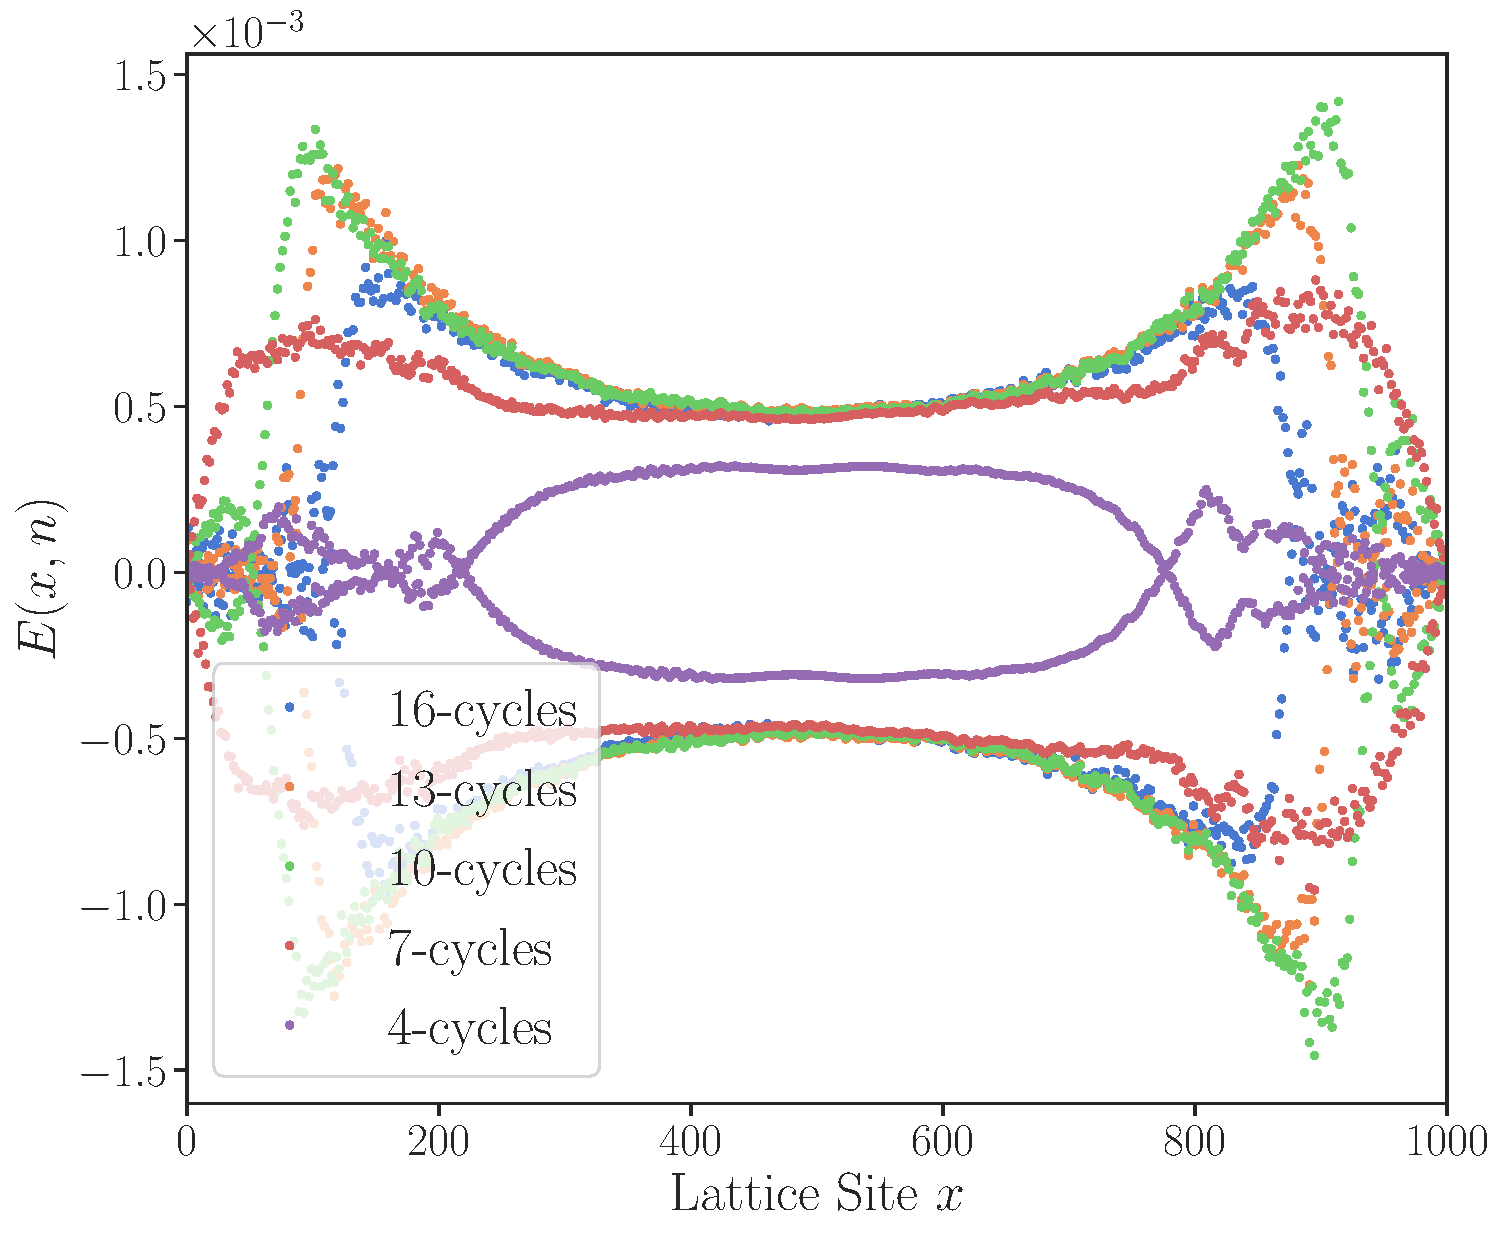
\includegraphics[width =\textwidth]{Energy_Density2}
\end{subfigure}
\caption{(left) (right)}
\end{figure}


\begin{figure}[h]
	\centering
	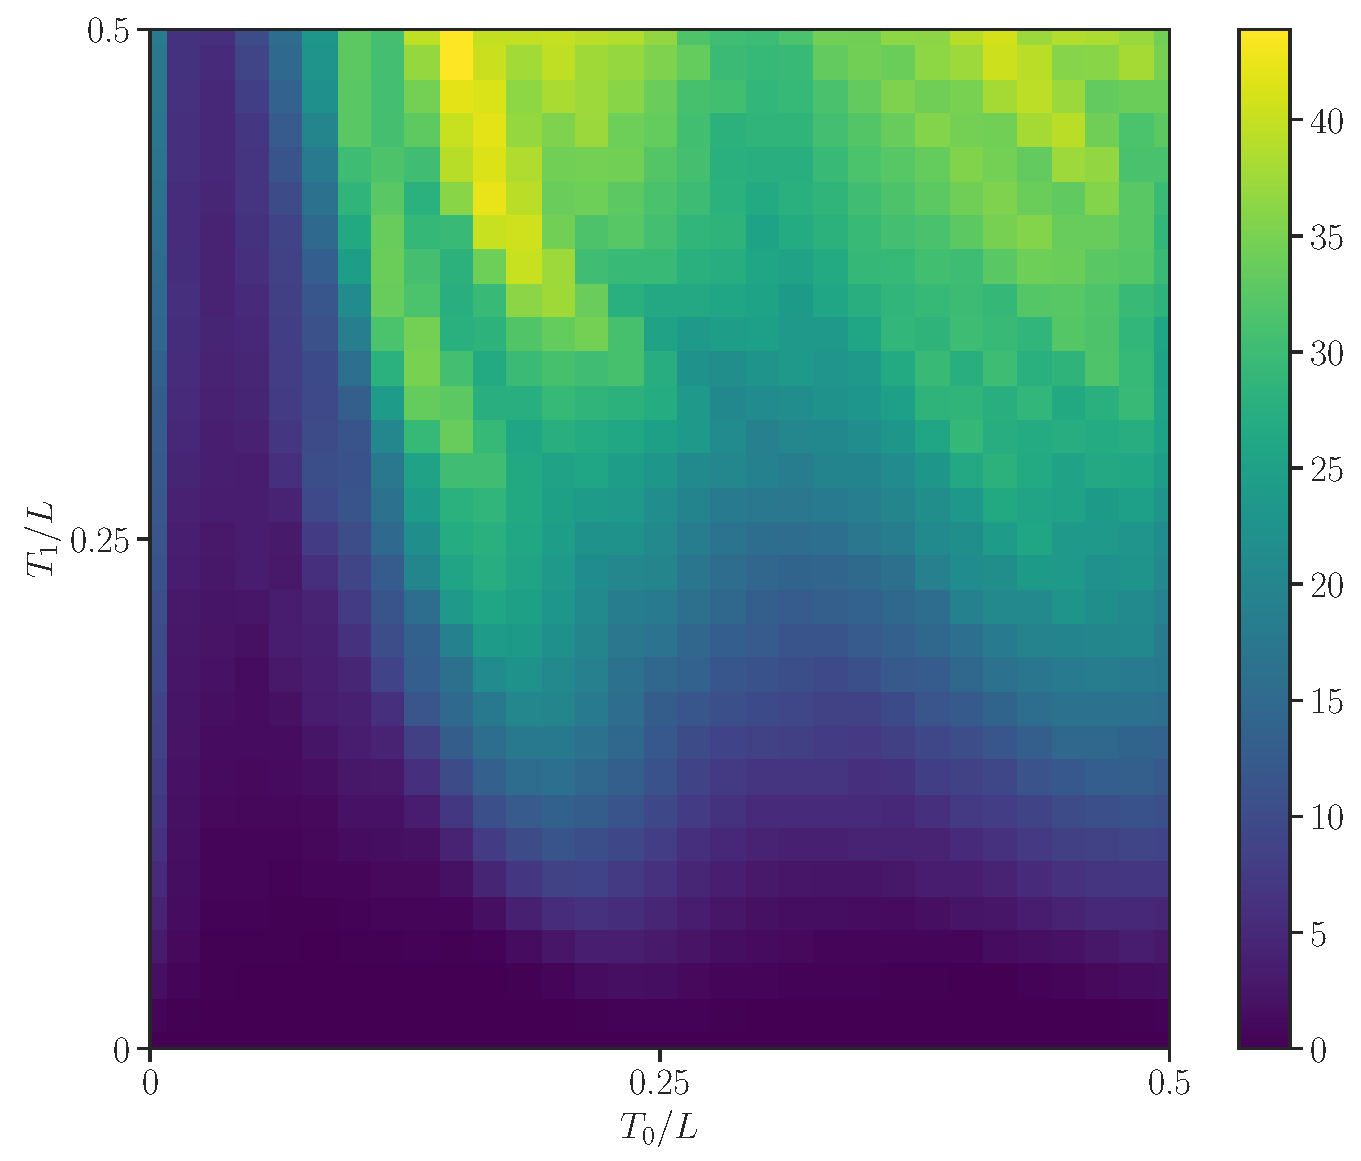
\includegraphics[width=0.8\textwidth]{PhaseDiagram2D}
	\caption{Phase Diagram for a 5-cycle driven two-dimensional square lattice with $L=15$, $5$ cycles and periodic boundary conditions.}
\end{figure}


\begin{figure}[h]
\centering
\begin{subfigure}[t]{0.49\textwidth}
	\centering
	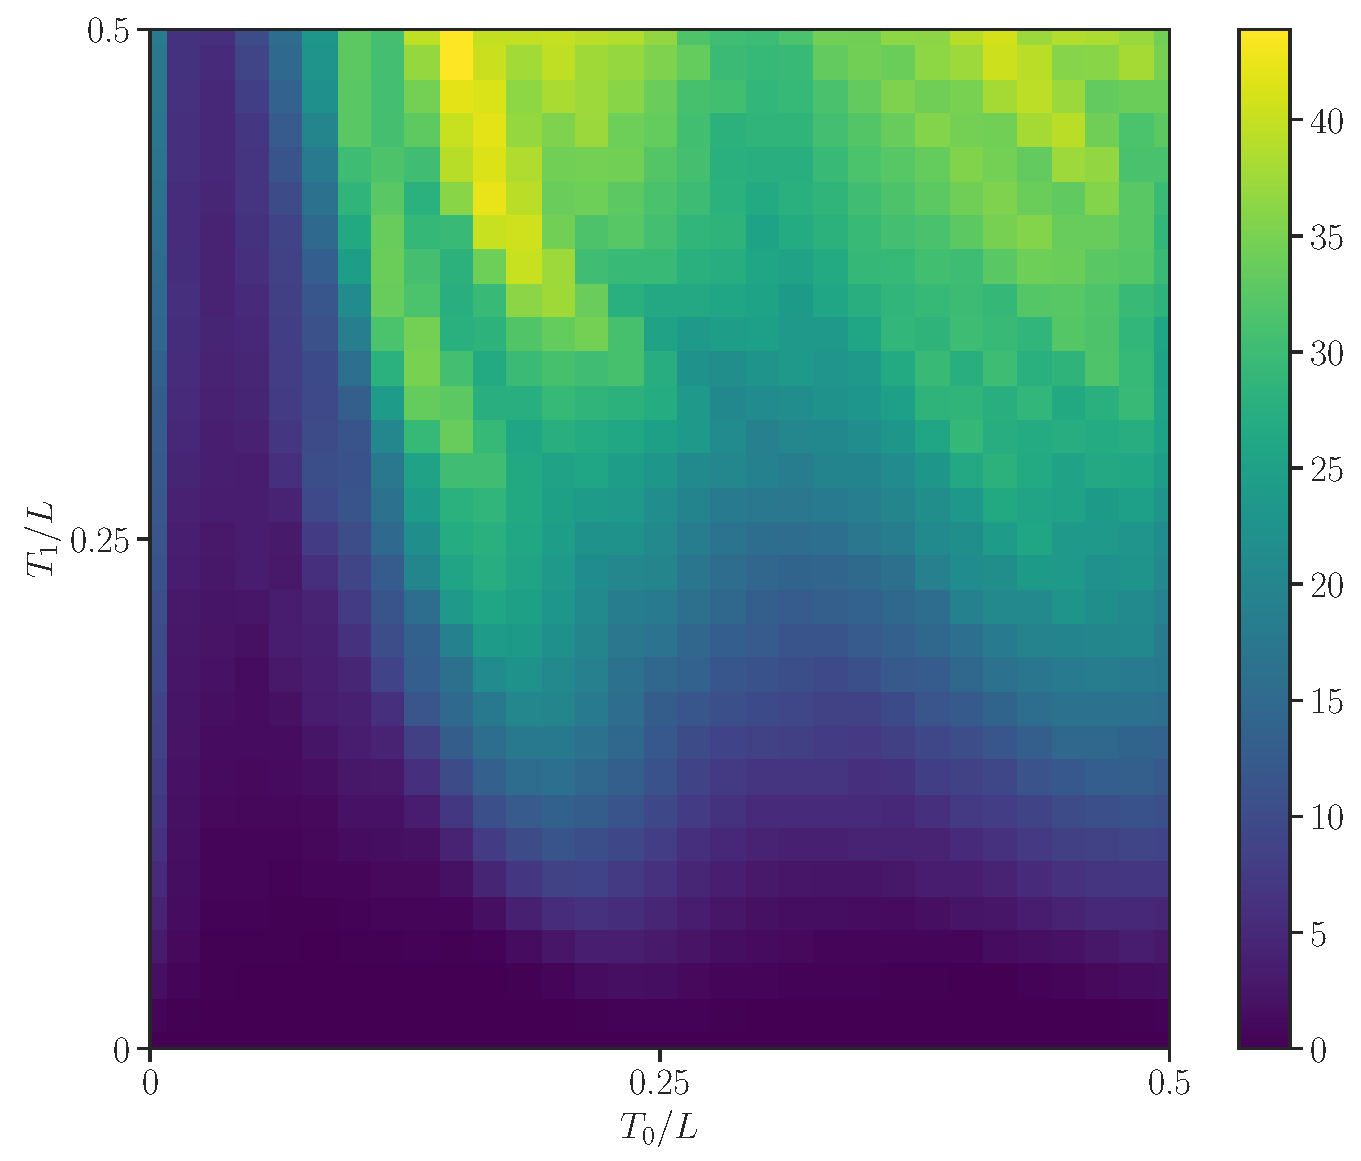
\includegraphics[width =\textwidth]{PhaseDiagram2D}
\end{subfigure}
\begin{subfigure}[t]{0.49\textwidth}
	\centering
	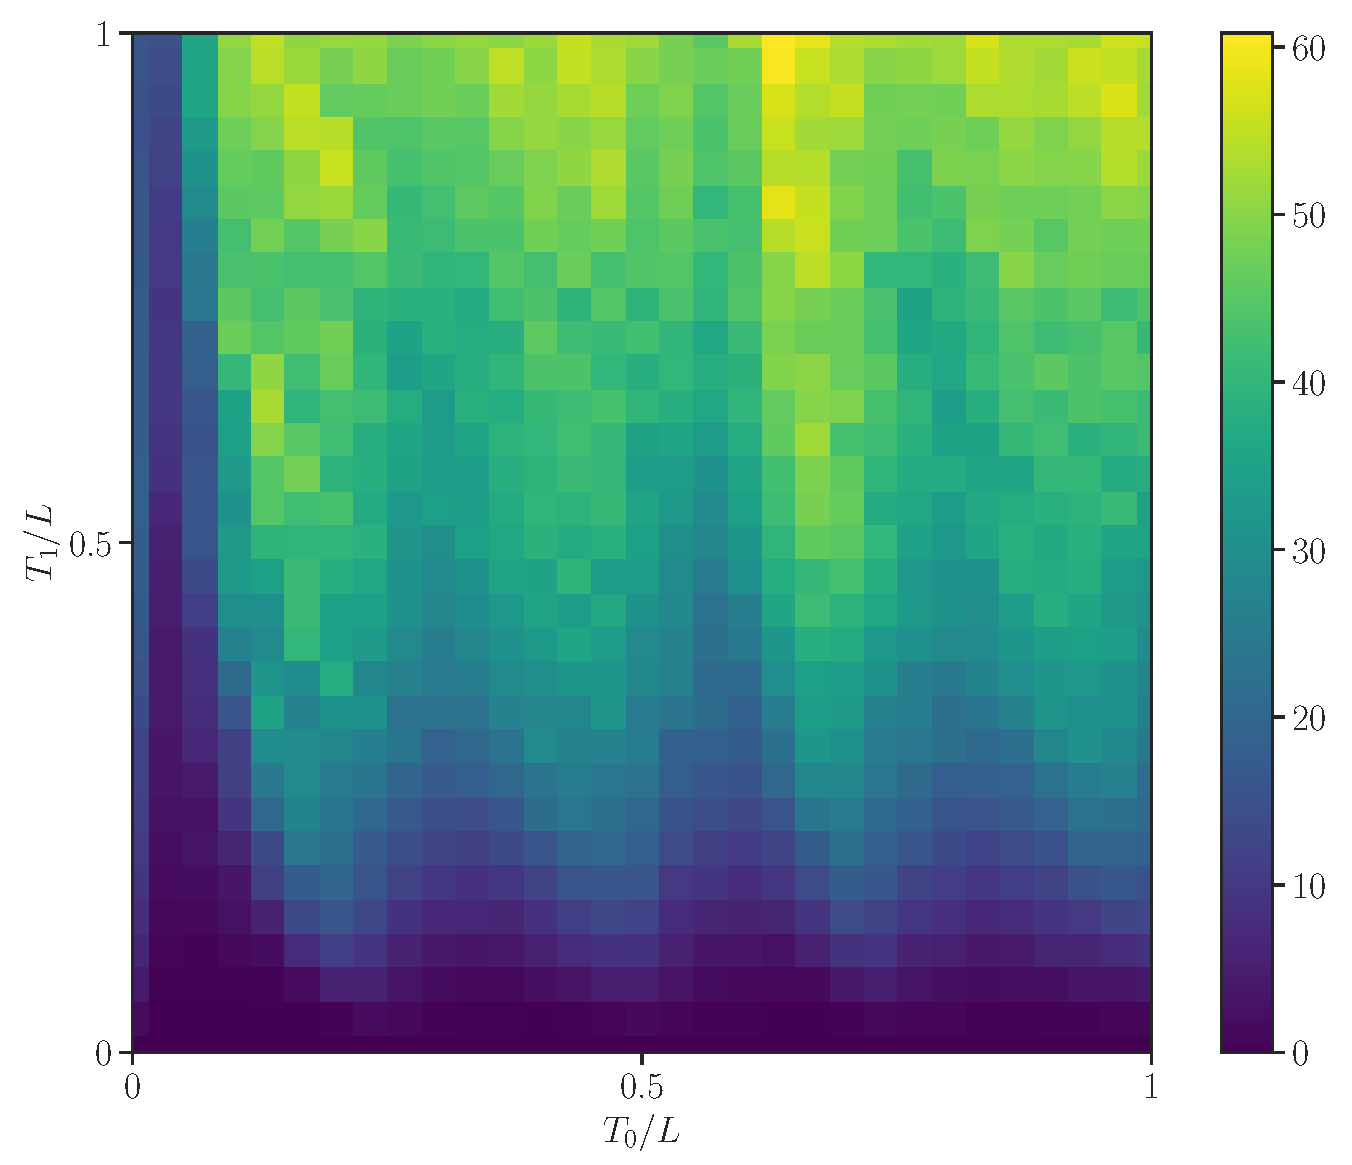
\includegraphics[width =\textwidth]{PhaseDiagram2D-2}
\end{subfigure}
\caption{(left) (right)}
\end{figure}


\begin{figure}[h]
	\centering
	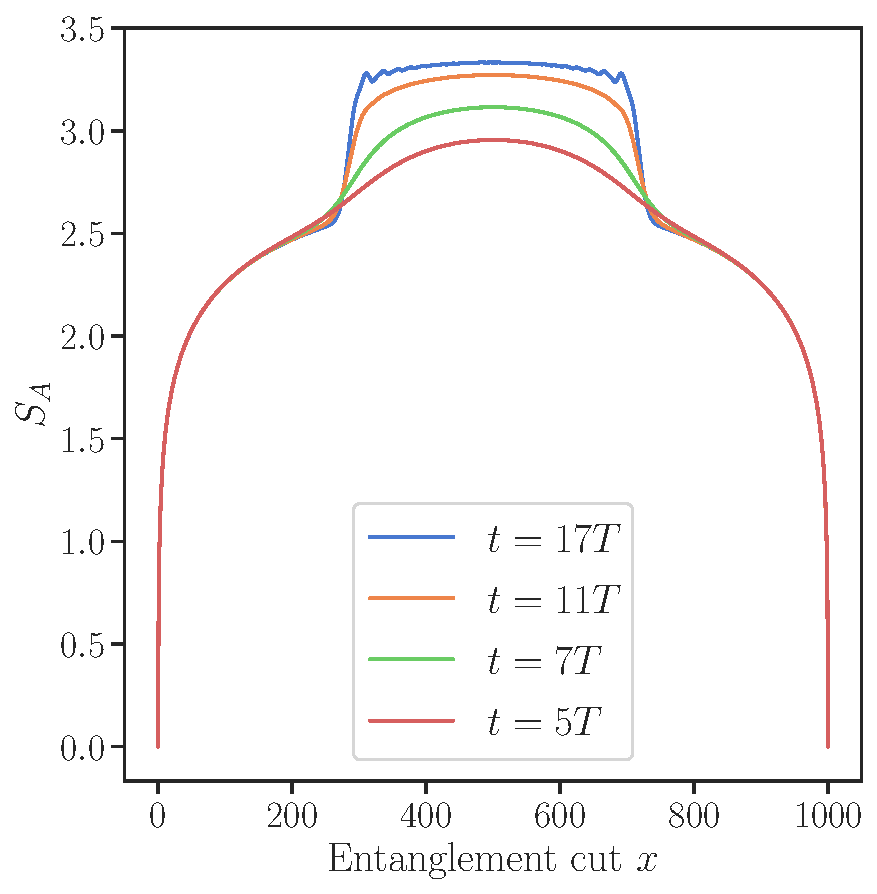
\includegraphics[width=0.8\textwidth]{Entanglement_Entropy}
	\caption{Evolution of entanglement entropy as a function of the entanglement cut $x$ for the subsystem $A[0:x]$. The Floquet system parameters are $T_0 = 0.95L$ and $T_1=0.05L$ and we have periodic boundary conditions.}
\end{figure}

\begin{figure}[h]
\centering
\begin{subfigure}[t]{0.49\textwidth}
	\centering
	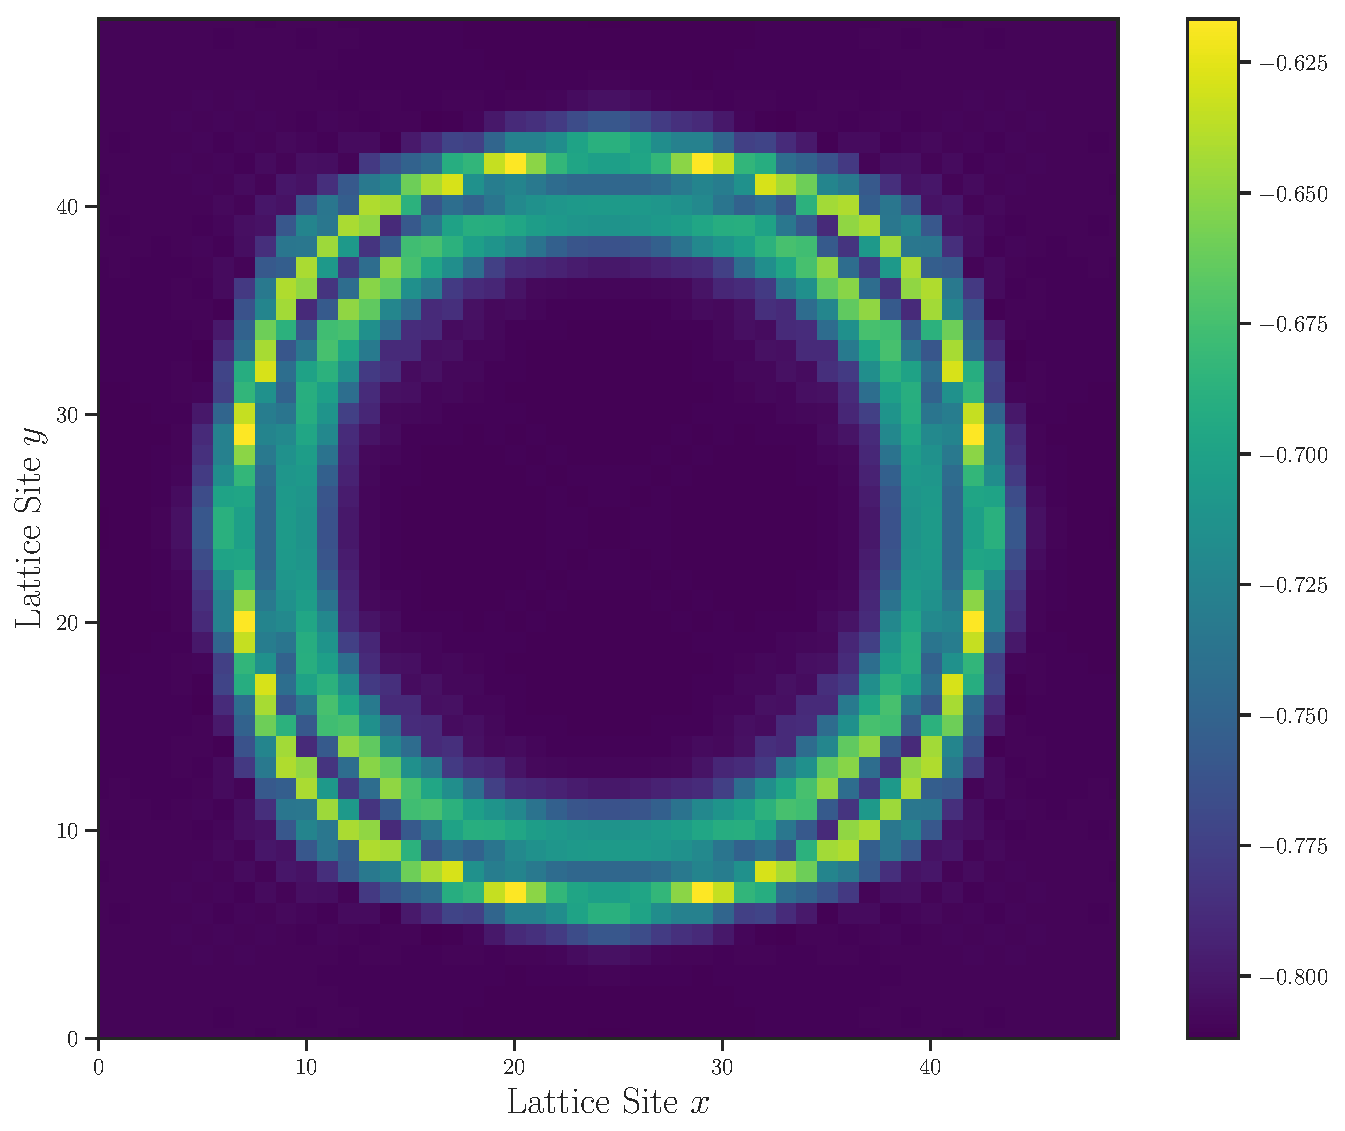
\includegraphics[width =\textwidth]{Energydensity2d_nearest.pdf}
\end{subfigure}
\begin{subfigure}[t]{0.49\textwidth}
	\centering
	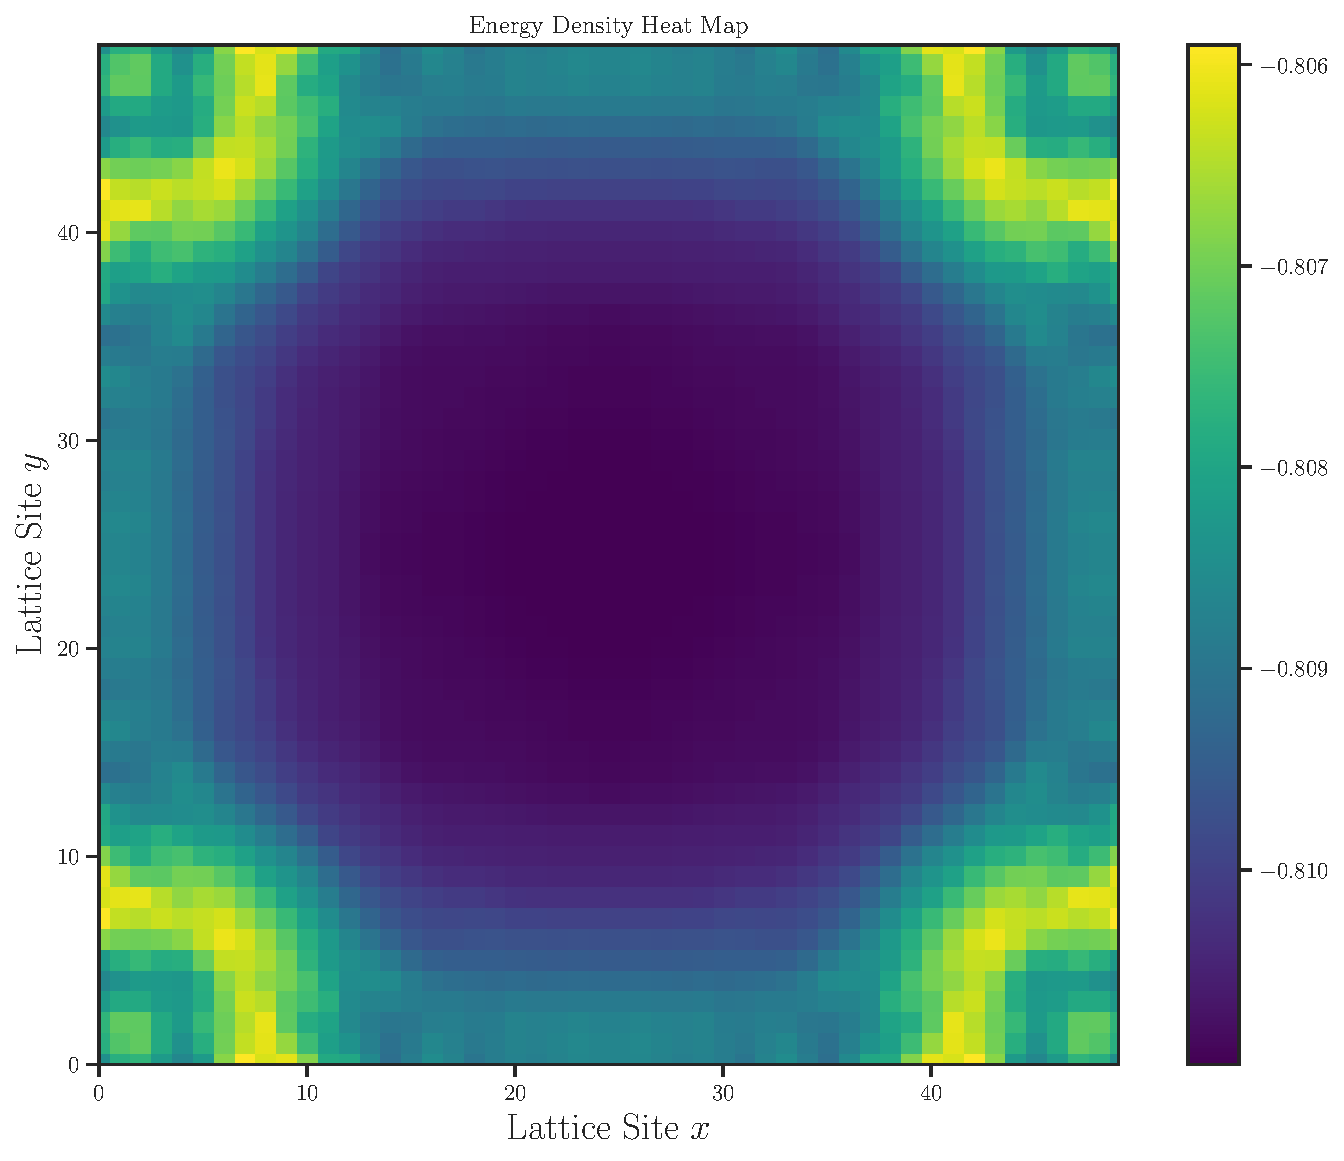
\includegraphics[width =\textwidth]{Energy_Density2D_nearest2.pdf}
\end{subfigure}
\caption{(left) (right)}
\end{figure}





\begin{figure}[h]
\centering
\begin{subfigure}[t]{0.49\textwidth}
	\centering
	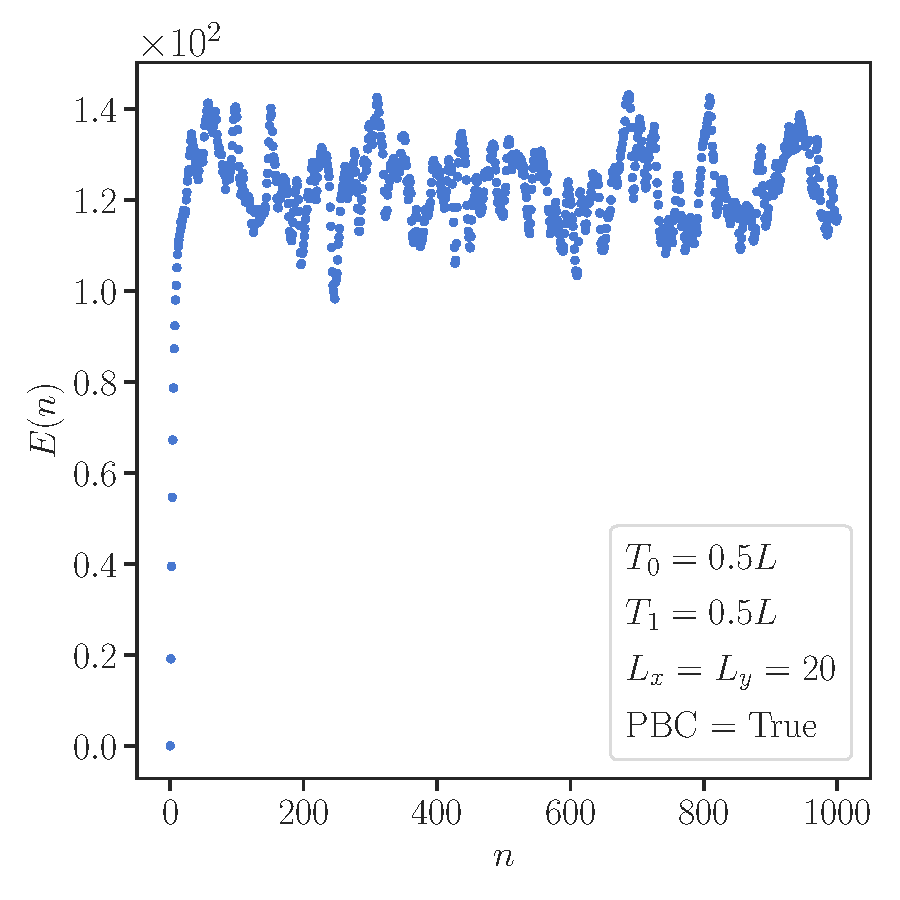
\includegraphics[width =\textwidth]{TotalEnergyHeating2d}
\end{subfigure}
\begin{subfigure}[t]{0.49\textwidth}
	\centering
	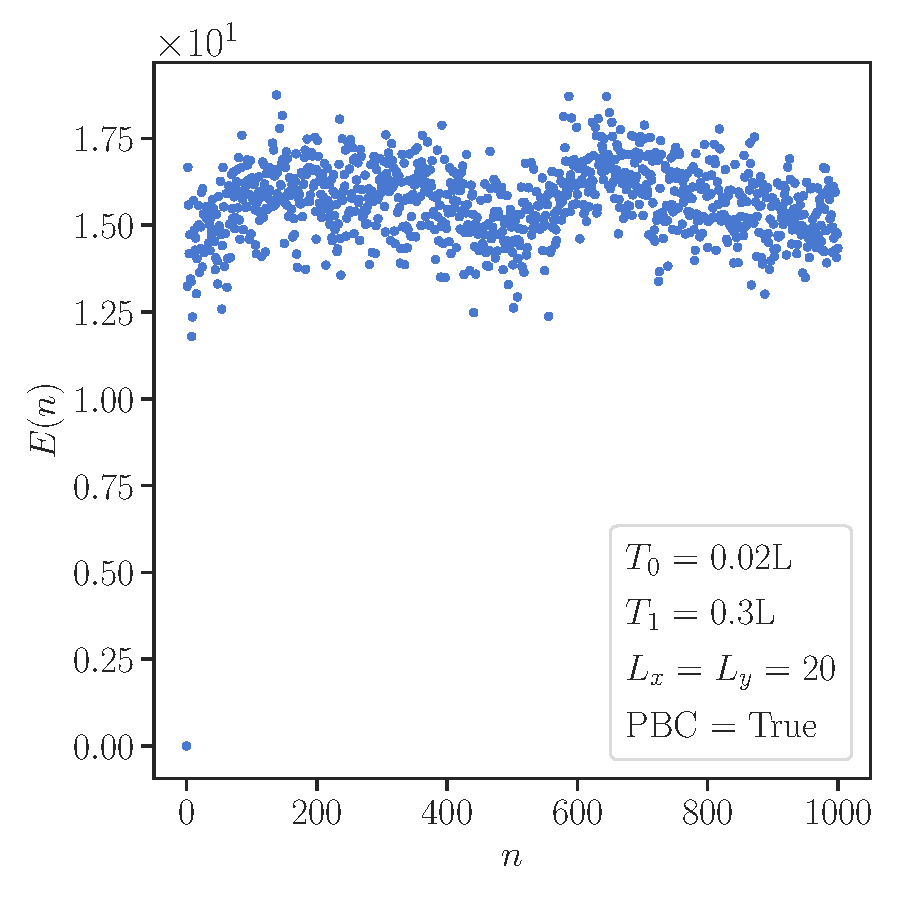
\includegraphics[width =\textwidth]{TotalEnergyNonHeating2d}
\end{subfigure}
\caption{(left) Total Energy Evolution as a function of the cycles for a heating phase (right)}
\end{figure}


\begin{figure}[h]
\centering
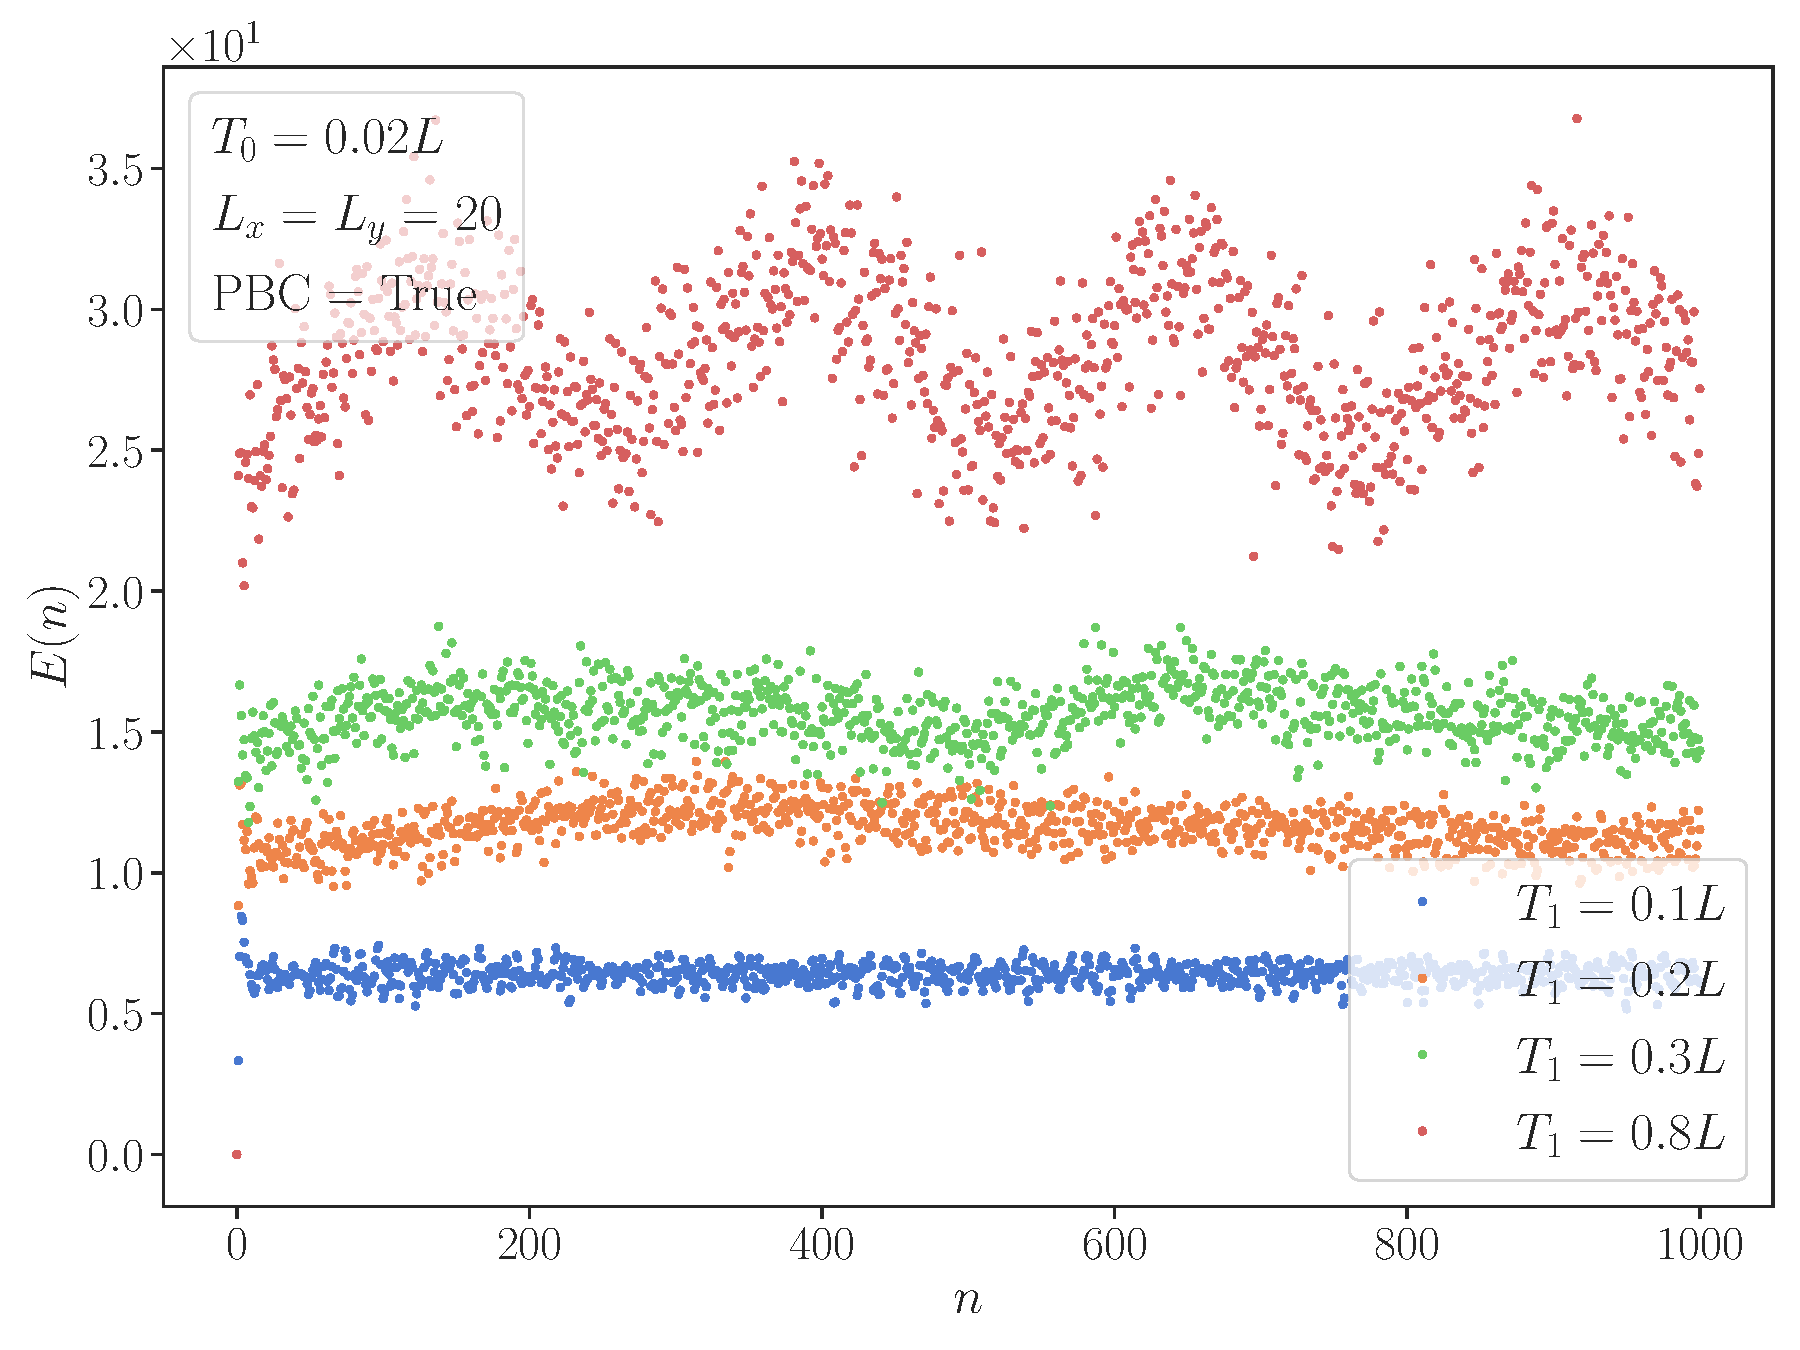
\includegraphics[width = 0.85\textwidth]{TotalEnergyNonHeating2d_Multiple}
\caption{Evolution of Total Energy $E(n)$ for the two-dimensional Floquet System as a function of the number of cycles $n$ for different parameters of $T_1$.}
\end{figure}


\begin{figure}[h]
\centering
		\begin{subfigure}[b]{0.31\textwidth}
			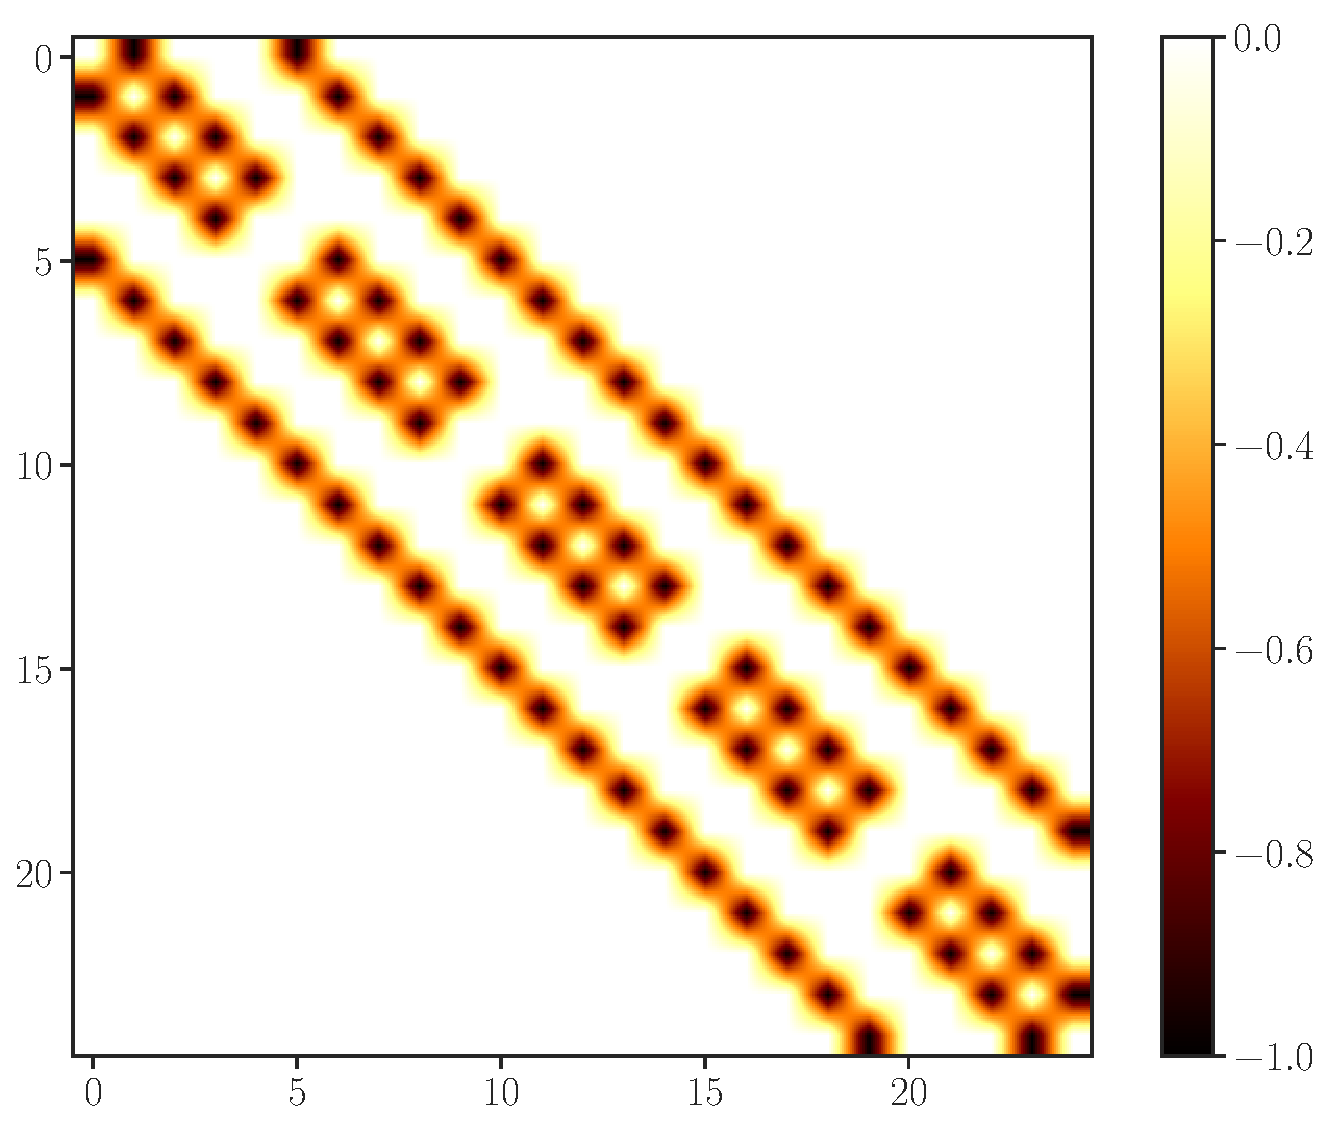
\includegraphics[width=\textwidth]{ColorMapMatrix_OBC_2D}
			\caption{}
		\end{subfigure}
		\begin{subfigure}[b]{0.31\textwidth}
			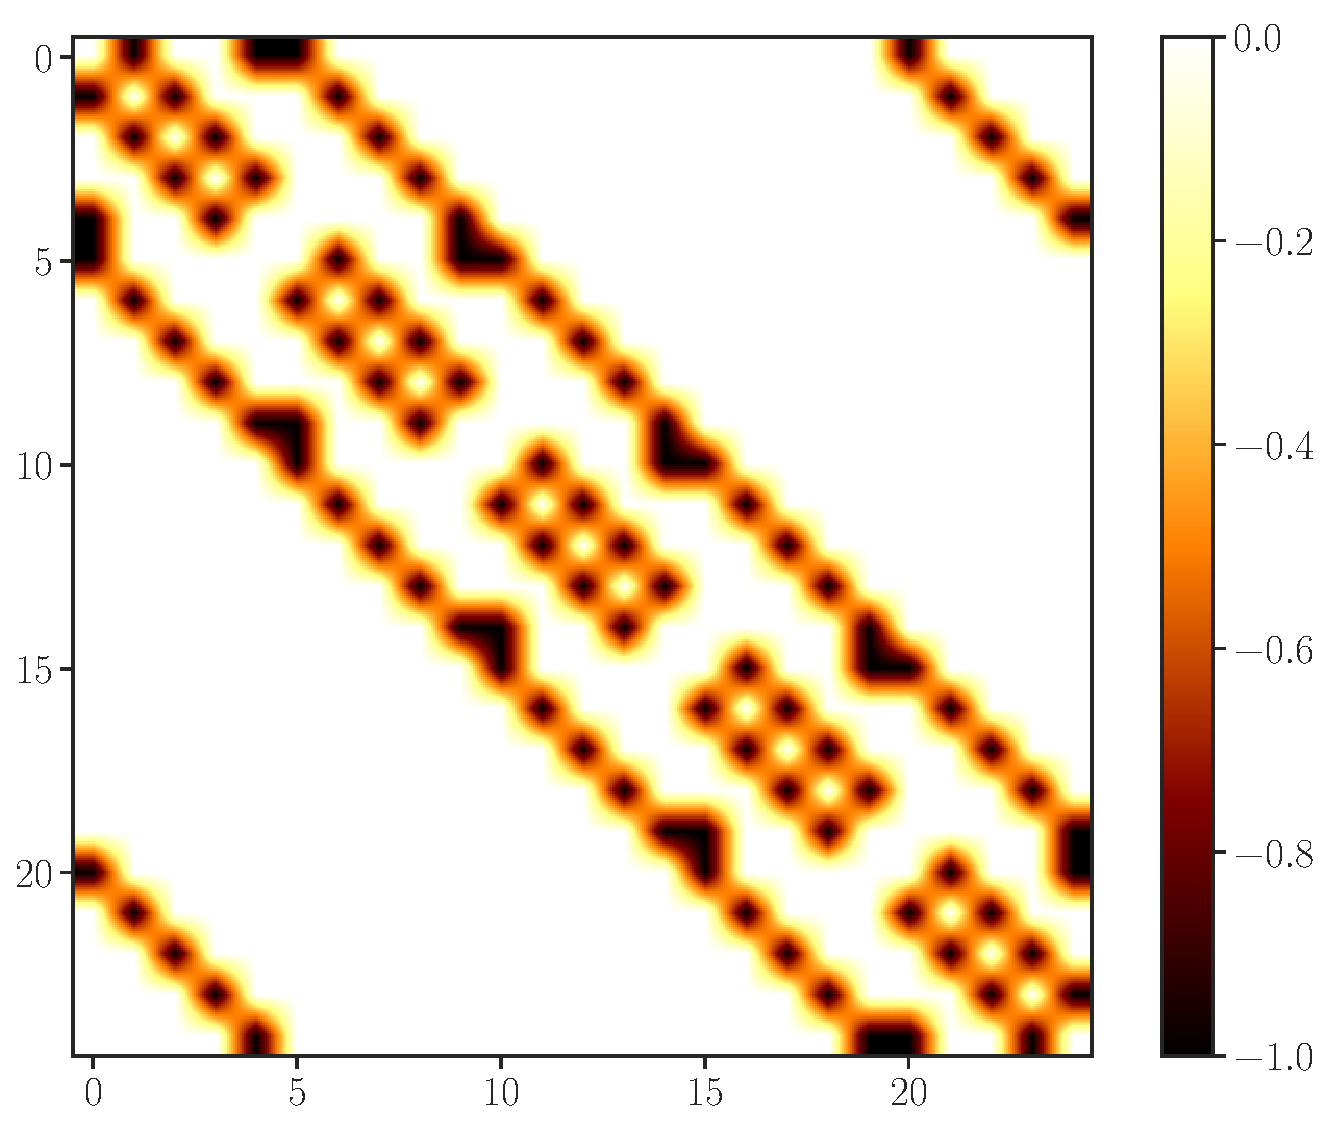
\includegraphics[width=\textwidth]{ColorMapMatrix_PBC_2D}
			\caption{}
		\end{subfigure}
		\begin{subfigure}[b]{0.31\textwidth}
			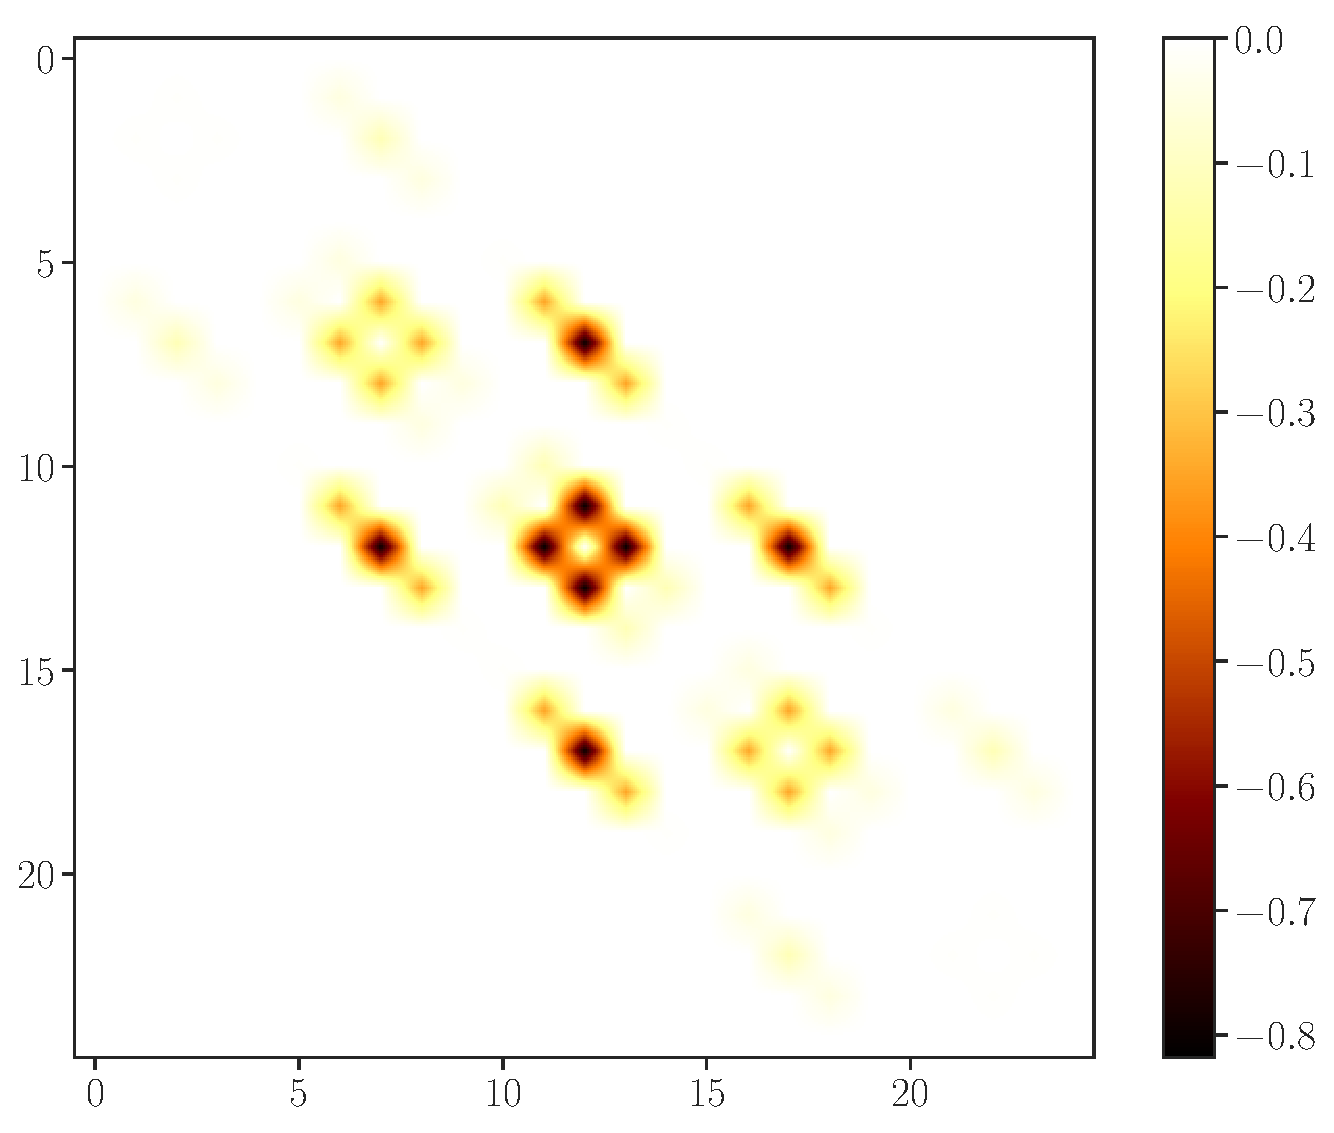
\includegraphics[width = \textwidth]{ColorMapMatrix_SSD_2D}	
			\caption{}
		\end{subfigure}
		\caption{Structure of the tight-binding Hamiltonian for $L_x = L_y = 5$ and (a) open-boundary conditions (b) periodic-boundary conditions (c) sine-squared deformed.}
\end{figure}




\begin{figure}[h]
\centering
		\begin{subfigure}[b]{0.45\textwidth}
			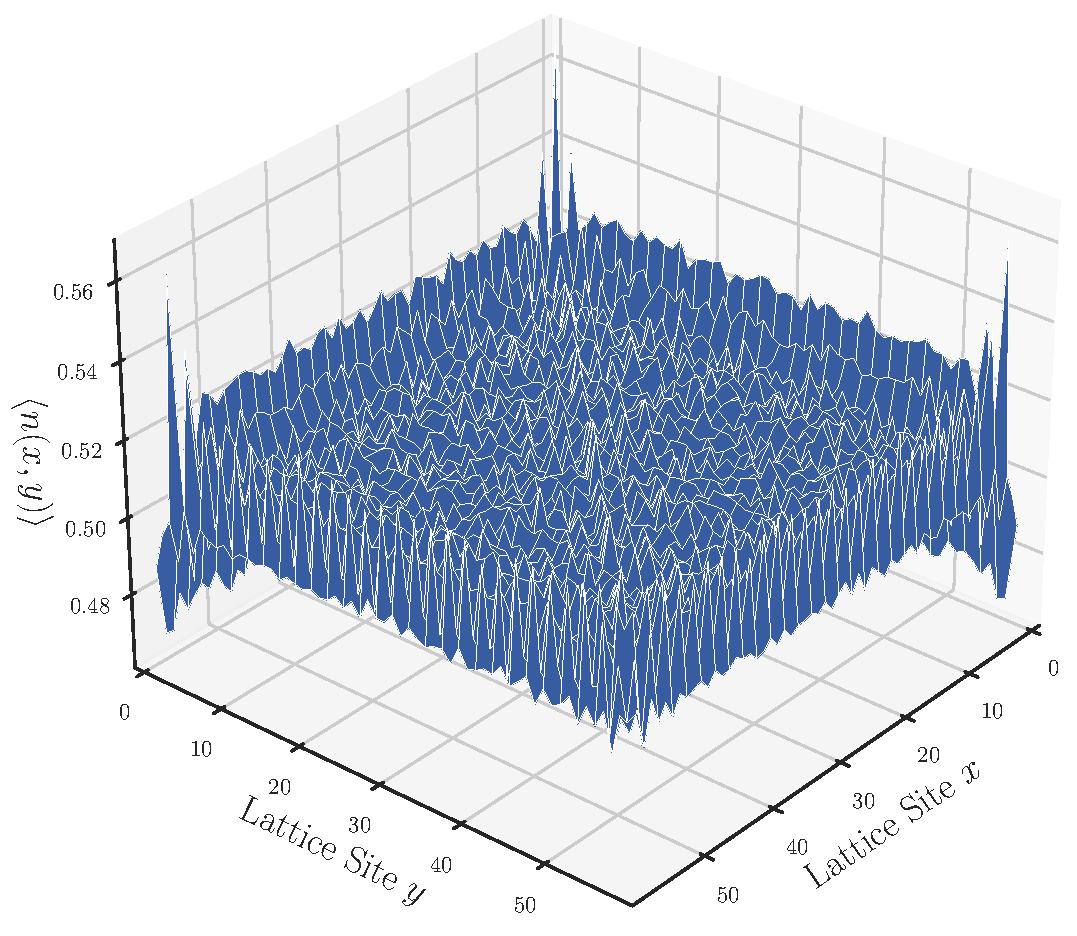
\includegraphics[width=\textwidth]{DensityprofileOBC}
			\caption{}
		\end{subfigure}
		\begin{subfigure}[b]{0.45\textwidth}
			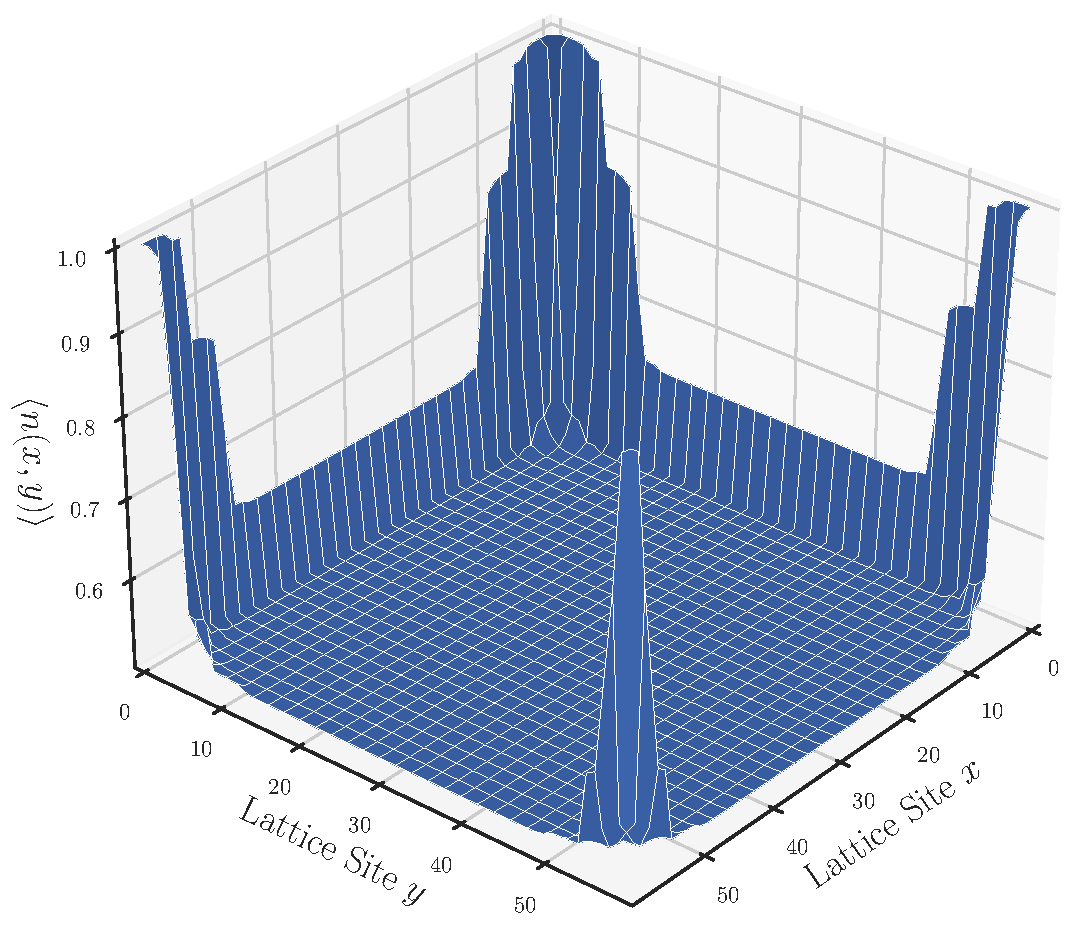
\includegraphics[width=\textwidth]{DensityprofileSSD}
			\caption{}
		\end{subfigure}
		\caption{Density profile $\expval{n(x,y)} = \sum_{i (E_i < 0)} \abs{\varphi_{i}(x,y)}^2$ of the groundstate for (a) open boundary conditions, (b) sine squared deformed.}
\end{figure}



\begin{figure}
\centering
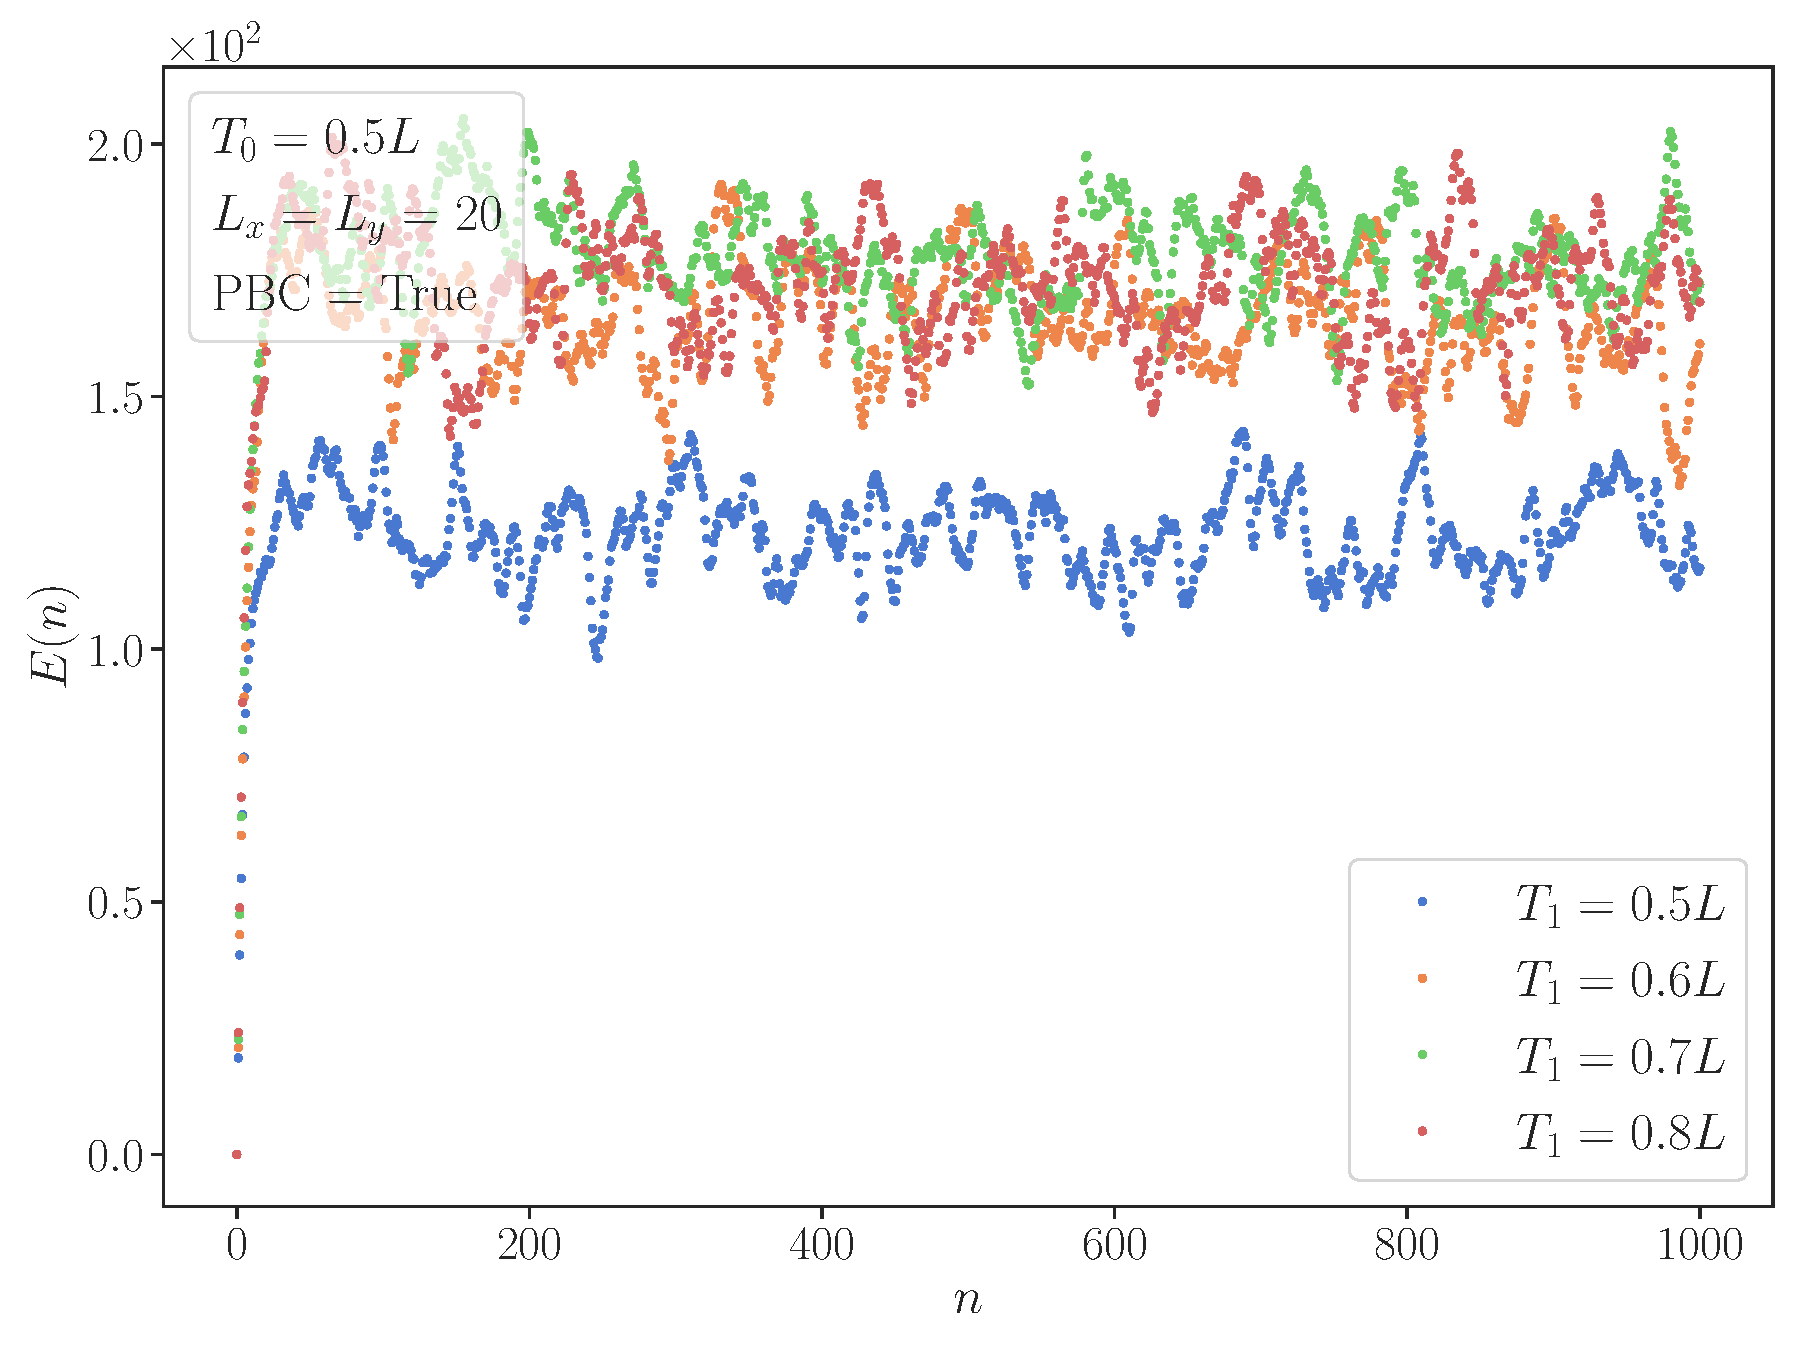
\includegraphics[width = 0.85\textwidth]{TotalEnergyHeating2d_Multiple}
\caption{}
\end{figure}
%



\begin{figure}[h]
\centering
\begin{subfigure}[t]{0.49\textwidth}
	\centering
	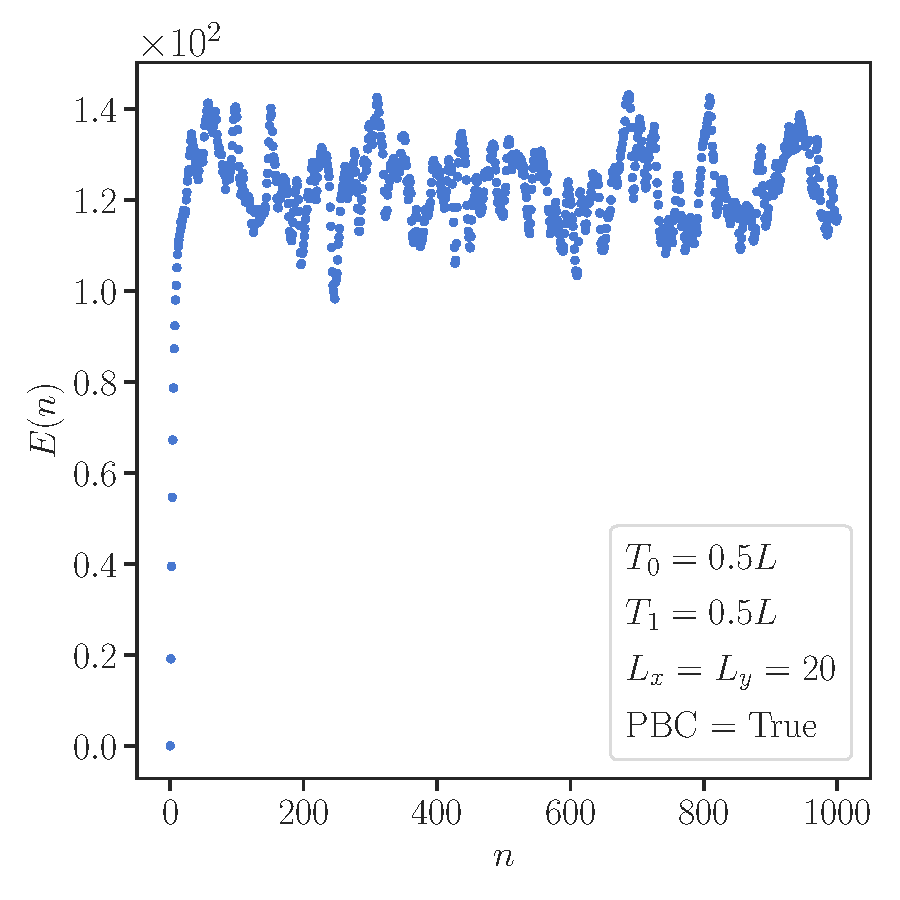
\includegraphics[width =\textwidth]{TotalEnergyHeating2d}
\end{subfigure}
\begin{subfigure}[t]{0.49\textwidth}
	\centering
	\includegraphics[width =\textwidth]{TotalEnergyNonHeating2d}
\end{subfigure}
\caption{(left) Total Energy Evolution as a function of the cycles for a heating phase (right)}
\end{figure}


%\begin{subfigure}{.5\textwidth}
%  \centering
%  \includegraphics[width=\linewidth]{Energy_Density2D_1}  
%  \caption{Put your sub-caption here}
%\end{subfigure}
%\begin{subfigure}{.5\textwidth}
%  \centering
%  \includegraphics[width=.8\linewidth]{log_demo2.png}  
%  \caption{Put your sub-caption here}
%\end{subfigure}
%
%\newline
%
%\begin{subfigure}{.5\textwidth}
%  \centering
%  \includegraphics[width=.8\linewidth]{log_demo1.png}  
%  \caption{Put your sub-caption here}
%\end{subfigure}
%\begin{subfigure}{.5\textwidth}
%  \centering
%  \includegraphics[width=.8\linewidth]{log_demo2.png}  
%  \caption{Put your sub-caption here}
%  \label{fig:sub-fourth}
%\end{subfigure}
%\caption{Put your caption here}
%\end{figure}


\newpage
\printbibliography[heading=bibintoc,title={Bibliography}]

\end{document}
